\documentclass[a4paper,10pt]{report}
\usepackage[utf8]{inputenc}

%multiline comments
\usepackage{verbatim}

%derivatives, ...
\usepackage{physics}

%for images
\usepackage{pgf}
\usepackage{tikz}
\usetikzlibrary{shapes,snakes}
\usetikzlibrary{backgrounds}
\usepackage{subfig}

%math symbols
\usepackage{amsmath}
\usepackage{amssymb}

%SI package
\usepackage{siunitx}

%line between paragraphs
\usepackage[parfill]{parskip}

\usepackage{geometry}
 \geometry{
 a4paper,
 total={160mm,227mm},
 left=30mm,
 right=30mm,
 top=30mm,
 }

%code listing
\usepackage{listings}

%linked toc
\usepackage[bookmarks]{hyperref}

%tables
\usepackage{booktabs}

\usepackage{enumitem}
\setlist[itemize]{align=parleft,left=0pt..1em}

%opening
\title{Design of a machine learning model for the detection of young planets}
\author{Alessandro Ruzza}

\begin{document}

\maketitle

\addcontentsline{toc}{chapter}{Abstract}
\begin{abstract}
    Protoplanetary discs present substructures,
    such as axisymmetric regions of luminosity depletion (gaps),
    that can be explained by the presence of forming planets. 
    Features of these objects can be inferred from their
    observation and analysis. A remarkable example is the 
    estimation of the planetary mass from the gaps morphology.
    The approaches currently used, empirical formulae or numerical
    simulations, are both limited in precision or applicability.
    In this thesis we propose a machine learning approach:
    using a neural network to infer this information from 
    disk images with the requirement of the least amount
    of physical features not directly observable.
    Possible future developments of such models require 
    data for the train and test phases.
    We design and build a database for this purpose collecting 
    data obtained from numerical simulations and providing an 
    easy-to-use interface for the implementation of machine learning
    models using TensorFlow libraries.
\end{abstract}

\tableofcontents

\chapter{Introduction}


\chapter{Protoplanetary discs}
%Very brief introduction (1/2 sentences) about what a protoplanetary disc is,
%how they generate, where we can find them and why they are studied.

Protoplanetary discs emerge in the context of star formation. 
The process takes place in specific ``star forming'' regions filled with a mixture of gases, mainly hydrogen and helium enriched with some
heavier elements, called interstellar medium. The gravitational collapse of a denser zone gives birth to a star. Gradually the star
accrete its mass drawing, from its surroundings, gas and dust that organizes in an accretion disc whose shape is a consequence of angular momentum conservation.
At some point, after $\sim 10^5$ yr, most of the matter has accreted into the star,
the disc temperature and thermal emission are maintained by the star irradiation while gravitational collapse becomes negligible as a source of energy (passive disc). 
It is at this stage that the accretion disc gets identified
as a protoplanetary disc due to its role as a planet formation cradle.
Their study allows the development and test of theoretical models regarding planets and their genesis.

In this chapter I am going to give an overview of the structure and observable features
of protoplanetary discs and of their relation with young embedded planets. The discussion will not be
exhaustive and neither detailed, the aim is to give
the reader a picture of these objects, and provide a basic understanding of the 
properties which I will be referring to in the next chapters.

\section{Structural properties}

\begin{figure}
    \begin{center}
    \raisebox{+0.2\height}{
        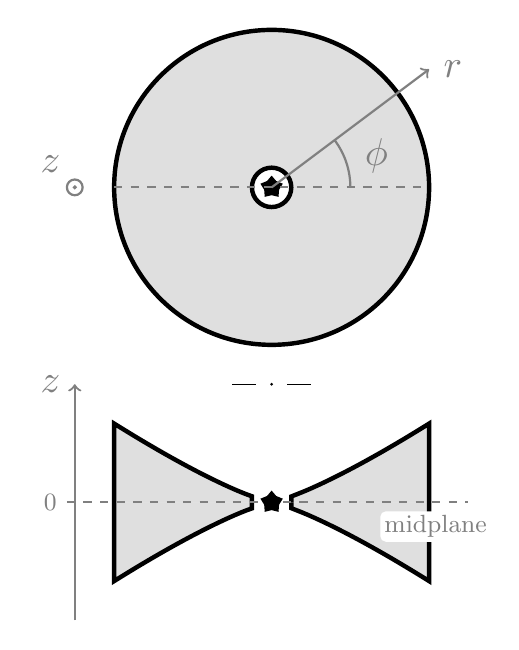
\begin{tikzpicture}
            \draw[ultra thick, color=black, domain=0.25:2, fill=gray, fill opacity=0.25] (0.25,0) -- plot (\x,{(\x*0.5)^(5/4)}) -- (2,0);
            \draw[ultra thick,color=black, domain=-2:-0.25, fill=gray, fill opacity=0.25] (-2,0) -- plot (\x,{(-\x*0.5)^(5/4)}) -- (-0.25, 0);
            \draw[ultra thick,color=black, domain=0.25:2, fill=gray, fill opacity=0.25] (0.25,0) -- plot (\x,{-(\x*0.5)^(5/4)}) -- (2,0);
            \draw[ultra thick,color=black, domain=-2:-0.25, fill=gray, fill opacity=0.25] (-2,0) -- plot (\x,{-(-\x*0.5)^(5/4)}) -- (-0.25,0);
            \draw[ultra thick,color=black] (2, 1) -- (2,-0.1);
            \draw[ultra thick,color=black] (2, -1) -- (2,-0.45);
            \draw[ultra thick,color=black] (-2, 1) -- (-2,-1);
            \draw[ thick,->, color=gray] (-2.5, -1.5) -- (-2.5, 1.5) node[left, scale=1.4] {$z$};
            \draw[ thick,color=gray, dashed] (-2.6, 0) node[left] {\small 0} -- (2.5, 0) node[below left, yshift=-1mm, xshift=3mm,  fill=white, rounded corners=2pt,inner sep=1.5pt] {\small midplane};
            \draw[ultra thick, fill=gray, fill opacity=0.25] (0,4) circle [radius=2cm];
            \draw[ultra thick, fill=white] (0,4) circle [radius=0.25cm];
            \node[star, fill=black, scale=0.6] at (0,4) {};
            \draw[ thick,color=gray] (-2.5,4) circle [radius=1mm] node[above left, scale=1.4] {$z$};
            \draw[ thick,color=gray, fill=gray] (-2.5,4) circle [radius=0.1mm];
            \draw[ thick,->, color=gray] (0,4) -- (2, 5.5) node[right, scale=1.4] {$r$};
            \draw[ thick,color=gray] (1,4) node[above right, scale=1.4] {$\phi$} arc (0:36.5:1cm);
            \draw[ thick,color=gray, dashed] (-2, 4) -- (2,4);
            \node[star, fill=black, scale=0.6] at (0,0) {};
            \draw[thin] (0, 1.5) circle [radius=0.1mm];
            \draw[thin] (0.2, 1.5) -- (0.5, 1.5);
            \draw[thin] (-0.2, 1.5) -- (-0.5, 1.5);
            %\draw[thin] (3, 1.5) circle [radius=0.1mm];
            %\draw[thin] (3, 1.3) -- (3, 1);
            %\draw[thin] (3, 1.7) -- (3, 2);
        \end{tikzpicture}}
        %\quadd
    %% Creator: Matplotlib, PGF backend
%%
%% To include the figure in your LaTeX document, write
%%   \input{<filename>.pgf}
%%
%% Make sure the required packages are loaded in your preamble
%%   \usepackage{pgf}
%%
%% Figures using additional raster images can only be included by \input if
%% they are in the same directory as the main LaTeX file. For loading figures
%% from other directories you can use the `import` package
%%   \usepackage{import}
%%
%% and then include the figures with
%%   \import{<path to file>}{<filename>.pgf}
%%
%% Matplotlib used the following preamble
%%
\begingroup%
\makeatletter%
\begin{pgfpicture}%
\pgfpathrectangle{\pgfpointorigin}{\pgfqpoint{3.380901in}{3.900000in}}%
\pgfusepath{use as bounding box, clip}%
\begin{pgfscope}%
\pgfsetbuttcap%
\pgfsetmiterjoin%
\pgfsetlinewidth{0.000000pt}%
\definecolor{currentstroke}{rgb}{1.000000,1.000000,1.000000}%
\pgfsetstrokecolor{currentstroke}%
\pgfsetstrokeopacity{0.000000}%
\pgfsetdash{}{0pt}%
\pgfpathmoveto{\pgfqpoint{0.000000in}{0.000000in}}%
\pgfpathlineto{\pgfqpoint{3.380901in}{0.000000in}}%
\pgfpathlineto{\pgfqpoint{3.380901in}{3.900000in}}%
\pgfpathlineto{\pgfqpoint{0.000000in}{3.900000in}}%
\pgfpathclose%
\pgfusepath{}%
\end{pgfscope}%
\begin{pgfscope}%
\pgfsetbuttcap%
\pgfsetmiterjoin%
\definecolor{currentfill}{rgb}{1.000000,1.000000,1.000000}%
\pgfsetfillcolor{currentfill}%
\pgfsetlinewidth{0.000000pt}%
\definecolor{currentstroke}{rgb}{0.000000,0.000000,0.000000}%
\pgfsetstrokecolor{currentstroke}%
\pgfsetstrokeopacity{0.000000}%
\pgfsetdash{}{0pt}%
\pgfpathmoveto{\pgfqpoint{0.746606in}{0.515123in}}%
\pgfpathlineto{\pgfqpoint{2.364932in}{0.515123in}}%
\pgfpathlineto{\pgfqpoint{2.364932in}{3.751775in}}%
\pgfpathlineto{\pgfqpoint{0.746606in}{3.751775in}}%
\pgfpathclose%
\pgfusepath{fill}%
\end{pgfscope}%
\begin{pgfscope}%
\pgfpathrectangle{\pgfqpoint{0.746606in}{0.515123in}}{\pgfqpoint{1.618326in}{3.236651in}}%
\pgfusepath{clip}%
\pgfsys@transformshift{0.746606in}{0.515123in}%
\pgftext[left,bottom]{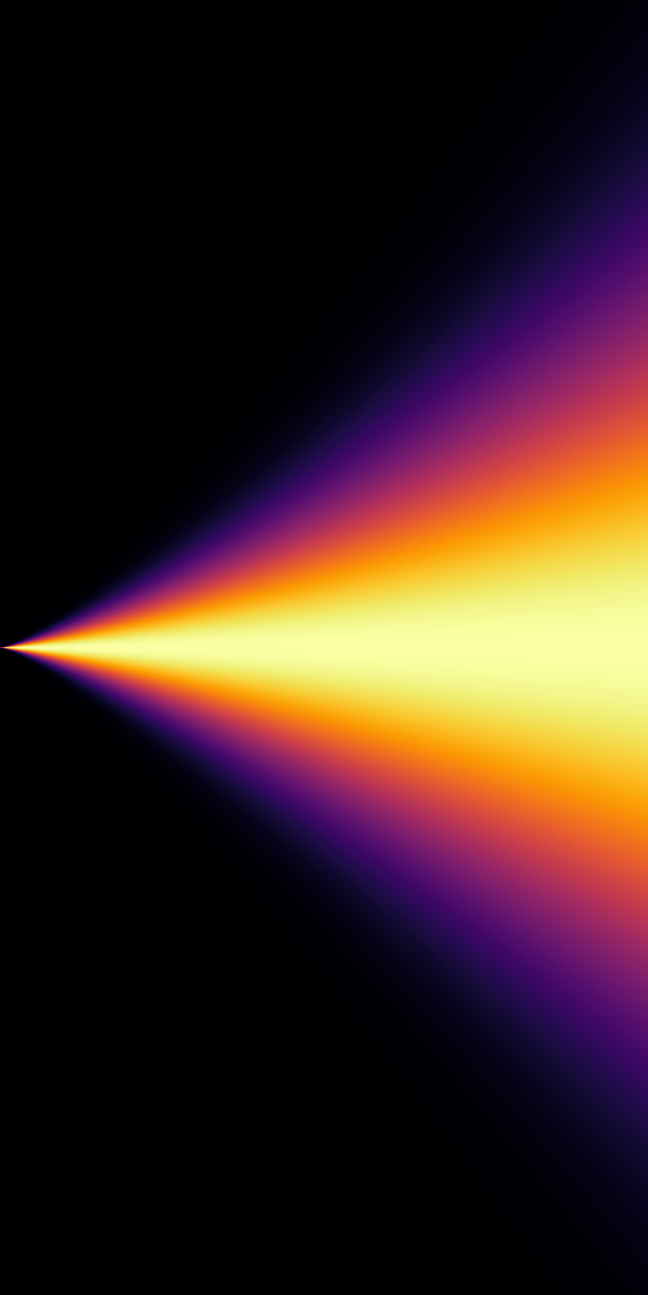
\includegraphics[interpolate=true,width=1.620000in,height=3.237500in]{images/profile-img0.png}}%
\end{pgfscope}%
\begin{pgfscope}%
\pgfsetbuttcap%
\pgfsetroundjoin%
\definecolor{currentfill}{rgb}{0.000000,0.000000,0.000000}%
\pgfsetfillcolor{currentfill}%
\pgfsetlinewidth{0.803000pt}%
\definecolor{currentstroke}{rgb}{0.000000,0.000000,0.000000}%
\pgfsetstrokecolor{currentstroke}%
\pgfsetdash{}{0pt}%
\pgfsys@defobject{currentmarker}{\pgfqpoint{0.000000in}{-0.048611in}}{\pgfqpoint{0.000000in}{0.000000in}}{%
\pgfpathmoveto{\pgfqpoint{0.000000in}{0.000000in}}%
\pgfpathlineto{\pgfqpoint{0.000000in}{-0.048611in}}%
\pgfusepath{stroke,fill}%
}%
\begin{pgfscope}%
\pgfsys@transformshift{0.746606in}{0.515123in}%
\pgfsys@useobject{currentmarker}{}%
\end{pgfscope}%
\end{pgfscope}%
\begin{pgfscope}%
\definecolor{textcolor}{rgb}{0.000000,0.000000,0.000000}%
\pgfsetstrokecolor{textcolor}%
\pgfsetfillcolor{textcolor}%
\pgftext[x=0.746606in,y=0.417901in,,top]{\color{textcolor}\rmfamily\fontsize{10.000000}{12.000000}\selectfont \(\displaystyle {0.0}\)}%
\end{pgfscope}%
\begin{pgfscope}%
\pgfsetbuttcap%
\pgfsetroundjoin%
\definecolor{currentfill}{rgb}{0.000000,0.000000,0.000000}%
\pgfsetfillcolor{currentfill}%
\pgfsetlinewidth{0.803000pt}%
\definecolor{currentstroke}{rgb}{0.000000,0.000000,0.000000}%
\pgfsetstrokecolor{currentstroke}%
\pgfsetdash{}{0pt}%
\pgfsys@defobject{currentmarker}{\pgfqpoint{0.000000in}{-0.048611in}}{\pgfqpoint{0.000000in}{0.000000in}}{%
\pgfpathmoveto{\pgfqpoint{0.000000in}{0.000000in}}%
\pgfpathlineto{\pgfqpoint{0.000000in}{-0.048611in}}%
\pgfusepath{stroke,fill}%
}%
\begin{pgfscope}%
\pgfsys@transformshift{1.555769in}{0.515123in}%
\pgfsys@useobject{currentmarker}{}%
\end{pgfscope}%
\end{pgfscope}%
\begin{pgfscope}%
\definecolor{textcolor}{rgb}{0.000000,0.000000,0.000000}%
\pgfsetstrokecolor{textcolor}%
\pgfsetfillcolor{textcolor}%
\pgftext[x=1.555769in,y=0.417901in,,top]{\color{textcolor}\rmfamily\fontsize{10.000000}{12.000000}\selectfont \(\displaystyle {0.5}\)}%
\end{pgfscope}%
\begin{pgfscope}%
\pgfsetbuttcap%
\pgfsetroundjoin%
\definecolor{currentfill}{rgb}{0.000000,0.000000,0.000000}%
\pgfsetfillcolor{currentfill}%
\pgfsetlinewidth{0.803000pt}%
\definecolor{currentstroke}{rgb}{0.000000,0.000000,0.000000}%
\pgfsetstrokecolor{currentstroke}%
\pgfsetdash{}{0pt}%
\pgfsys@defobject{currentmarker}{\pgfqpoint{0.000000in}{-0.048611in}}{\pgfqpoint{0.000000in}{0.000000in}}{%
\pgfpathmoveto{\pgfqpoint{0.000000in}{0.000000in}}%
\pgfpathlineto{\pgfqpoint{0.000000in}{-0.048611in}}%
\pgfusepath{stroke,fill}%
}%
\begin{pgfscope}%
\pgfsys@transformshift{2.364932in}{0.515123in}%
\pgfsys@useobject{currentmarker}{}%
\end{pgfscope}%
\end{pgfscope}%
\begin{pgfscope}%
\definecolor{textcolor}{rgb}{0.000000,0.000000,0.000000}%
\pgfsetstrokecolor{textcolor}%
\pgfsetfillcolor{textcolor}%
\pgftext[x=2.364932in,y=0.417901in,,top]{\color{textcolor}\rmfamily\fontsize{10.000000}{12.000000}\selectfont \(\displaystyle {1.0}\)}%
\end{pgfscope}%
\begin{pgfscope}%
\definecolor{textcolor}{rgb}{0.000000,0.000000,0.000000}%
\pgfsetstrokecolor{textcolor}%
\pgfsetfillcolor{textcolor}%
\pgftext[x=1.555769in,y=0.238889in,,top]{\color{textcolor}\rmfamily\fontsize{10.000000}{12.000000}\selectfont \(\displaystyle r\) [arb. unit]}%
\end{pgfscope}%
\begin{pgfscope}%
\pgfsetbuttcap%
\pgfsetroundjoin%
\definecolor{currentfill}{rgb}{0.000000,0.000000,0.000000}%
\pgfsetfillcolor{currentfill}%
\pgfsetlinewidth{0.803000pt}%
\definecolor{currentstroke}{rgb}{0.000000,0.000000,0.000000}%
\pgfsetstrokecolor{currentstroke}%
\pgfsetdash{}{0pt}%
\pgfsys@defobject{currentmarker}{\pgfqpoint{-0.048611in}{0.000000in}}{\pgfqpoint{-0.000000in}{0.000000in}}{%
\pgfpathmoveto{\pgfqpoint{-0.000000in}{0.000000in}}%
\pgfpathlineto{\pgfqpoint{-0.048611in}{0.000000in}}%
\pgfusepath{stroke,fill}%
}%
\begin{pgfscope}%
\pgfsys@transformshift{0.746606in}{0.515123in}%
\pgfsys@useobject{currentmarker}{}%
\end{pgfscope}%
\end{pgfscope}%
\begin{pgfscope}%
\definecolor{textcolor}{rgb}{0.000000,0.000000,0.000000}%
\pgfsetstrokecolor{textcolor}%
\pgfsetfillcolor{textcolor}%
\pgftext[x=0.294444in, y=0.466898in, left, base]{\color{textcolor}\rmfamily\fontsize{10.000000}{12.000000}\selectfont \(\displaystyle {\ensuremath{-}1.00}\)}%
\end{pgfscope}%
\begin{pgfscope}%
\pgfsetbuttcap%
\pgfsetroundjoin%
\definecolor{currentfill}{rgb}{0.000000,0.000000,0.000000}%
\pgfsetfillcolor{currentfill}%
\pgfsetlinewidth{0.803000pt}%
\definecolor{currentstroke}{rgb}{0.000000,0.000000,0.000000}%
\pgfsetstrokecolor{currentstroke}%
\pgfsetdash{}{0pt}%
\pgfsys@defobject{currentmarker}{\pgfqpoint{-0.048611in}{0.000000in}}{\pgfqpoint{-0.000000in}{0.000000in}}{%
\pgfpathmoveto{\pgfqpoint{-0.000000in}{0.000000in}}%
\pgfpathlineto{\pgfqpoint{-0.048611in}{0.000000in}}%
\pgfusepath{stroke,fill}%
}%
\begin{pgfscope}%
\pgfsys@transformshift{0.746606in}{0.919705in}%
\pgfsys@useobject{currentmarker}{}%
\end{pgfscope}%
\end{pgfscope}%
\begin{pgfscope}%
\definecolor{textcolor}{rgb}{0.000000,0.000000,0.000000}%
\pgfsetstrokecolor{textcolor}%
\pgfsetfillcolor{textcolor}%
\pgftext[x=0.294444in, y=0.871479in, left, base]{\color{textcolor}\rmfamily\fontsize{10.000000}{12.000000}\selectfont \(\displaystyle {\ensuremath{-}0.75}\)}%
\end{pgfscope}%
\begin{pgfscope}%
\pgfsetbuttcap%
\pgfsetroundjoin%
\definecolor{currentfill}{rgb}{0.000000,0.000000,0.000000}%
\pgfsetfillcolor{currentfill}%
\pgfsetlinewidth{0.803000pt}%
\definecolor{currentstroke}{rgb}{0.000000,0.000000,0.000000}%
\pgfsetstrokecolor{currentstroke}%
\pgfsetdash{}{0pt}%
\pgfsys@defobject{currentmarker}{\pgfqpoint{-0.048611in}{0.000000in}}{\pgfqpoint{-0.000000in}{0.000000in}}{%
\pgfpathmoveto{\pgfqpoint{-0.000000in}{0.000000in}}%
\pgfpathlineto{\pgfqpoint{-0.048611in}{0.000000in}}%
\pgfusepath{stroke,fill}%
}%
\begin{pgfscope}%
\pgfsys@transformshift{0.746606in}{1.324286in}%
\pgfsys@useobject{currentmarker}{}%
\end{pgfscope}%
\end{pgfscope}%
\begin{pgfscope}%
\definecolor{textcolor}{rgb}{0.000000,0.000000,0.000000}%
\pgfsetstrokecolor{textcolor}%
\pgfsetfillcolor{textcolor}%
\pgftext[x=0.294444in, y=1.276061in, left, base]{\color{textcolor}\rmfamily\fontsize{10.000000}{12.000000}\selectfont \(\displaystyle {\ensuremath{-}0.50}\)}%
\end{pgfscope}%
\begin{pgfscope}%
\pgfsetbuttcap%
\pgfsetroundjoin%
\definecolor{currentfill}{rgb}{0.000000,0.000000,0.000000}%
\pgfsetfillcolor{currentfill}%
\pgfsetlinewidth{0.803000pt}%
\definecolor{currentstroke}{rgb}{0.000000,0.000000,0.000000}%
\pgfsetstrokecolor{currentstroke}%
\pgfsetdash{}{0pt}%
\pgfsys@defobject{currentmarker}{\pgfqpoint{-0.048611in}{0.000000in}}{\pgfqpoint{-0.000000in}{0.000000in}}{%
\pgfpathmoveto{\pgfqpoint{-0.000000in}{0.000000in}}%
\pgfpathlineto{\pgfqpoint{-0.048611in}{0.000000in}}%
\pgfusepath{stroke,fill}%
}%
\begin{pgfscope}%
\pgfsys@transformshift{0.746606in}{1.728868in}%
\pgfsys@useobject{currentmarker}{}%
\end{pgfscope}%
\end{pgfscope}%
\begin{pgfscope}%
\definecolor{textcolor}{rgb}{0.000000,0.000000,0.000000}%
\pgfsetstrokecolor{textcolor}%
\pgfsetfillcolor{textcolor}%
\pgftext[x=0.294444in, y=1.680642in, left, base]{\color{textcolor}\rmfamily\fontsize{10.000000}{12.000000}\selectfont \(\displaystyle {\ensuremath{-}0.25}\)}%
\end{pgfscope}%
\begin{pgfscope}%
\pgfsetbuttcap%
\pgfsetroundjoin%
\definecolor{currentfill}{rgb}{0.000000,0.000000,0.000000}%
\pgfsetfillcolor{currentfill}%
\pgfsetlinewidth{0.803000pt}%
\definecolor{currentstroke}{rgb}{0.000000,0.000000,0.000000}%
\pgfsetstrokecolor{currentstroke}%
\pgfsetdash{}{0pt}%
\pgfsys@defobject{currentmarker}{\pgfqpoint{-0.048611in}{0.000000in}}{\pgfqpoint{-0.000000in}{0.000000in}}{%
\pgfpathmoveto{\pgfqpoint{-0.000000in}{0.000000in}}%
\pgfpathlineto{\pgfqpoint{-0.048611in}{0.000000in}}%
\pgfusepath{stroke,fill}%
}%
\begin{pgfscope}%
\pgfsys@transformshift{0.746606in}{2.133449in}%
\pgfsys@useobject{currentmarker}{}%
\end{pgfscope}%
\end{pgfscope}%
\begin{pgfscope}%
\definecolor{textcolor}{rgb}{0.000000,0.000000,0.000000}%
\pgfsetstrokecolor{textcolor}%
\pgfsetfillcolor{textcolor}%
\pgftext[x=0.402469in, y=2.085224in, left, base]{\color{textcolor}\rmfamily\fontsize{10.000000}{12.000000}\selectfont \(\displaystyle {0.00}\)}%
\end{pgfscope}%
\begin{pgfscope}%
\pgfsetbuttcap%
\pgfsetroundjoin%
\definecolor{currentfill}{rgb}{0.000000,0.000000,0.000000}%
\pgfsetfillcolor{currentfill}%
\pgfsetlinewidth{0.803000pt}%
\definecolor{currentstroke}{rgb}{0.000000,0.000000,0.000000}%
\pgfsetstrokecolor{currentstroke}%
\pgfsetdash{}{0pt}%
\pgfsys@defobject{currentmarker}{\pgfqpoint{-0.048611in}{0.000000in}}{\pgfqpoint{-0.000000in}{0.000000in}}{%
\pgfpathmoveto{\pgfqpoint{-0.000000in}{0.000000in}}%
\pgfpathlineto{\pgfqpoint{-0.048611in}{0.000000in}}%
\pgfusepath{stroke,fill}%
}%
\begin{pgfscope}%
\pgfsys@transformshift{0.746606in}{2.538030in}%
\pgfsys@useobject{currentmarker}{}%
\end{pgfscope}%
\end{pgfscope}%
\begin{pgfscope}%
\definecolor{textcolor}{rgb}{0.000000,0.000000,0.000000}%
\pgfsetstrokecolor{textcolor}%
\pgfsetfillcolor{textcolor}%
\pgftext[x=0.402469in, y=2.489805in, left, base]{\color{textcolor}\rmfamily\fontsize{10.000000}{12.000000}\selectfont \(\displaystyle {0.25}\)}%
\end{pgfscope}%
\begin{pgfscope}%
\pgfsetbuttcap%
\pgfsetroundjoin%
\definecolor{currentfill}{rgb}{0.000000,0.000000,0.000000}%
\pgfsetfillcolor{currentfill}%
\pgfsetlinewidth{0.803000pt}%
\definecolor{currentstroke}{rgb}{0.000000,0.000000,0.000000}%
\pgfsetstrokecolor{currentstroke}%
\pgfsetdash{}{0pt}%
\pgfsys@defobject{currentmarker}{\pgfqpoint{-0.048611in}{0.000000in}}{\pgfqpoint{-0.000000in}{0.000000in}}{%
\pgfpathmoveto{\pgfqpoint{-0.000000in}{0.000000in}}%
\pgfpathlineto{\pgfqpoint{-0.048611in}{0.000000in}}%
\pgfusepath{stroke,fill}%
}%
\begin{pgfscope}%
\pgfsys@transformshift{0.746606in}{2.942612in}%
\pgfsys@useobject{currentmarker}{}%
\end{pgfscope}%
\end{pgfscope}%
\begin{pgfscope}%
\definecolor{textcolor}{rgb}{0.000000,0.000000,0.000000}%
\pgfsetstrokecolor{textcolor}%
\pgfsetfillcolor{textcolor}%
\pgftext[x=0.402469in, y=2.894387in, left, base]{\color{textcolor}\rmfamily\fontsize{10.000000}{12.000000}\selectfont \(\displaystyle {0.50}\)}%
\end{pgfscope}%
\begin{pgfscope}%
\pgfsetbuttcap%
\pgfsetroundjoin%
\definecolor{currentfill}{rgb}{0.000000,0.000000,0.000000}%
\pgfsetfillcolor{currentfill}%
\pgfsetlinewidth{0.803000pt}%
\definecolor{currentstroke}{rgb}{0.000000,0.000000,0.000000}%
\pgfsetstrokecolor{currentstroke}%
\pgfsetdash{}{0pt}%
\pgfsys@defobject{currentmarker}{\pgfqpoint{-0.048611in}{0.000000in}}{\pgfqpoint{-0.000000in}{0.000000in}}{%
\pgfpathmoveto{\pgfqpoint{-0.000000in}{0.000000in}}%
\pgfpathlineto{\pgfqpoint{-0.048611in}{0.000000in}}%
\pgfusepath{stroke,fill}%
}%
\begin{pgfscope}%
\pgfsys@transformshift{0.746606in}{3.347193in}%
\pgfsys@useobject{currentmarker}{}%
\end{pgfscope}%
\end{pgfscope}%
\begin{pgfscope}%
\definecolor{textcolor}{rgb}{0.000000,0.000000,0.000000}%
\pgfsetstrokecolor{textcolor}%
\pgfsetfillcolor{textcolor}%
\pgftext[x=0.402469in, y=3.298968in, left, base]{\color{textcolor}\rmfamily\fontsize{10.000000}{12.000000}\selectfont \(\displaystyle {0.75}\)}%
\end{pgfscope}%
\begin{pgfscope}%
\pgfsetbuttcap%
\pgfsetroundjoin%
\definecolor{currentfill}{rgb}{0.000000,0.000000,0.000000}%
\pgfsetfillcolor{currentfill}%
\pgfsetlinewidth{0.803000pt}%
\definecolor{currentstroke}{rgb}{0.000000,0.000000,0.000000}%
\pgfsetstrokecolor{currentstroke}%
\pgfsetdash{}{0pt}%
\pgfsys@defobject{currentmarker}{\pgfqpoint{-0.048611in}{0.000000in}}{\pgfqpoint{-0.000000in}{0.000000in}}{%
\pgfpathmoveto{\pgfqpoint{-0.000000in}{0.000000in}}%
\pgfpathlineto{\pgfqpoint{-0.048611in}{0.000000in}}%
\pgfusepath{stroke,fill}%
}%
\begin{pgfscope}%
\pgfsys@transformshift{0.746606in}{3.751775in}%
\pgfsys@useobject{currentmarker}{}%
\end{pgfscope}%
\end{pgfscope}%
\begin{pgfscope}%
\definecolor{textcolor}{rgb}{0.000000,0.000000,0.000000}%
\pgfsetstrokecolor{textcolor}%
\pgfsetfillcolor{textcolor}%
\pgftext[x=0.402469in, y=3.703549in, left, base]{\color{textcolor}\rmfamily\fontsize{10.000000}{12.000000}\selectfont \(\displaystyle {1.00}\)}%
\end{pgfscope}%
\begin{pgfscope}%
\definecolor{textcolor}{rgb}{0.000000,0.000000,0.000000}%
\pgfsetstrokecolor{textcolor}%
\pgfsetfillcolor{textcolor}%
\pgftext[x=0.238889in,y=2.133449in,,bottom,rotate=90.000000]{\color{textcolor}\rmfamily\fontsize{10.000000}{12.000000}\selectfont \(\displaystyle z\) [arb. unit]}%
\end{pgfscope}%
\begin{pgfscope}%
\pgfpathrectangle{\pgfqpoint{0.746606in}{0.515123in}}{\pgfqpoint{1.618326in}{3.236651in}}%
\pgfusepath{clip}%
\pgfsetbuttcap%
\pgfsetroundjoin%
\pgfsetlinewidth{1.505625pt}%
\definecolor{currentstroke}{rgb}{1.000000,1.000000,1.000000}%
\pgfsetstrokecolor{currentstroke}%
\pgfsetdash{{5.550000pt}{2.400000pt}}{0.000000pt}%
\pgfpathmoveto{\pgfqpoint{0.746606in}{2.133449in}}%
\pgfpathlineto{\pgfqpoint{0.751461in}{2.133978in}}%
\pgfpathlineto{\pgfqpoint{0.760362in}{2.135571in}}%
\pgfpathlineto{\pgfqpoint{0.771690in}{2.138177in}}%
\pgfpathlineto{\pgfqpoint{0.785446in}{2.141918in}}%
\pgfpathlineto{\pgfqpoint{0.801629in}{2.146924in}}%
\pgfpathlineto{\pgfqpoint{0.819431in}{2.153030in}}%
\pgfpathlineto{\pgfqpoint{0.838851in}{2.160286in}}%
\pgfpathlineto{\pgfqpoint{0.859889in}{2.168742in}}%
\pgfpathlineto{\pgfqpoint{0.882545in}{2.178455in}}%
\pgfpathlineto{\pgfqpoint{0.906820in}{2.189477in}}%
\pgfpathlineto{\pgfqpoint{0.932713in}{2.201865in}}%
\pgfpathlineto{\pgfqpoint{0.959416in}{2.215257in}}%
\pgfpathlineto{\pgfqpoint{0.987737in}{2.230086in}}%
\pgfpathlineto{\pgfqpoint{1.017676in}{2.246406in}}%
\pgfpathlineto{\pgfqpoint{1.048424in}{2.263805in}}%
\pgfpathlineto{\pgfqpoint{1.080790in}{2.282770in}}%
\pgfpathlineto{\pgfqpoint{1.113966in}{2.302855in}}%
\pgfpathlineto{\pgfqpoint{1.148760in}{2.324579in}}%
\pgfpathlineto{\pgfqpoint{1.184363in}{2.347467in}}%
\pgfpathlineto{\pgfqpoint{1.221585in}{2.372068in}}%
\pgfpathlineto{\pgfqpoint{1.259615in}{2.397876in}}%
\pgfpathlineto{\pgfqpoint{1.298455in}{2.424901in}}%
\pgfpathlineto{\pgfqpoint{1.338913in}{2.453733in}}%
\pgfpathlineto{\pgfqpoint{1.380180in}{2.483827in}}%
\pgfpathlineto{\pgfqpoint{1.423066in}{2.515800in}}%
\pgfpathlineto{\pgfqpoint{1.466761in}{2.549079in}}%
\pgfpathlineto{\pgfqpoint{1.511265in}{2.583674in}}%
\pgfpathlineto{\pgfqpoint{1.557387in}{2.620242in}}%
\pgfpathlineto{\pgfqpoint{1.604319in}{2.658170in}}%
\pgfpathlineto{\pgfqpoint{1.652059in}{2.697468in}}%
\pgfpathlineto{\pgfqpoint{1.700609in}{2.738148in}}%
\pgfpathlineto{\pgfqpoint{1.750777in}{2.780914in}}%
\pgfpathlineto{\pgfqpoint{1.801754in}{2.825106in}}%
\pgfpathlineto{\pgfqpoint{1.853541in}{2.870734in}}%
\pgfpathlineto{\pgfqpoint{1.906136in}{2.917809in}}%
\pgfpathlineto{\pgfqpoint{1.960350in}{2.967083in}}%
\pgfpathlineto{\pgfqpoint{2.015373in}{3.017849in}}%
\pgfpathlineto{\pgfqpoint{2.071206in}{3.070116in}}%
\pgfpathlineto{\pgfqpoint{2.127847in}{3.123897in}}%
\pgfpathlineto{\pgfqpoint{2.186107in}{3.179987in}}%
\pgfpathlineto{\pgfqpoint{2.245176in}{3.237634in}}%
\pgfpathlineto{\pgfqpoint{2.305054in}{3.296849in}}%
\pgfpathlineto{\pgfqpoint{2.364123in}{3.356011in}}%
\pgfpathlineto{\pgfqpoint{2.364123in}{3.356011in}}%
\pgfusepath{stroke}%
\end{pgfscope}%
\begin{pgfscope}%
\pgfsetrectcap%
\pgfsetmiterjoin%
\pgfsetlinewidth{0.803000pt}%
\definecolor{currentstroke}{rgb}{0.000000,0.000000,0.000000}%
\pgfsetstrokecolor{currentstroke}%
\pgfsetdash{}{0pt}%
\pgfpathmoveto{\pgfqpoint{0.746606in}{0.515123in}}%
\pgfpathlineto{\pgfqpoint{0.746606in}{3.751775in}}%
\pgfusepath{stroke}%
\end{pgfscope}%
\begin{pgfscope}%
\pgfsetrectcap%
\pgfsetmiterjoin%
\pgfsetlinewidth{0.803000pt}%
\definecolor{currentstroke}{rgb}{0.000000,0.000000,0.000000}%
\pgfsetstrokecolor{currentstroke}%
\pgfsetdash{}{0pt}%
\pgfpathmoveto{\pgfqpoint{2.364932in}{0.515123in}}%
\pgfpathlineto{\pgfqpoint{2.364932in}{3.751775in}}%
\pgfusepath{stroke}%
\end{pgfscope}%
\begin{pgfscope}%
\pgfsetrectcap%
\pgfsetmiterjoin%
\pgfsetlinewidth{0.803000pt}%
\definecolor{currentstroke}{rgb}{0.000000,0.000000,0.000000}%
\pgfsetstrokecolor{currentstroke}%
\pgfsetdash{}{0pt}%
\pgfpathmoveto{\pgfqpoint{0.746606in}{0.515123in}}%
\pgfpathlineto{\pgfqpoint{2.364932in}{0.515123in}}%
\pgfusepath{stroke}%
\end{pgfscope}%
\begin{pgfscope}%
\pgfsetrectcap%
\pgfsetmiterjoin%
\pgfsetlinewidth{0.803000pt}%
\definecolor{currentstroke}{rgb}{0.000000,0.000000,0.000000}%
\pgfsetstrokecolor{currentstroke}%
\pgfsetdash{}{0pt}%
\pgfpathmoveto{\pgfqpoint{0.746606in}{3.751775in}}%
\pgfpathlineto{\pgfqpoint{2.364932in}{3.751775in}}%
\pgfusepath{stroke}%
\end{pgfscope}%
\begin{pgfscope}%
\pgfsetbuttcap%
\pgfsetroundjoin%
\pgfsetlinewidth{1.505625pt}%
\definecolor{currentstroke}{rgb}{1.000000,1.000000,1.000000}%
\pgfsetstrokecolor{currentstroke}%
\pgfsetdash{{5.550000pt}{2.400000pt}}{0.000000pt}%
\pgfpathmoveto{\pgfqpoint{0.871606in}{0.723457in}}%
\pgfpathlineto{\pgfqpoint{1.149384in}{0.723457in}}%
\pgfusepath{stroke}%
\end{pgfscope}%
\begin{pgfscope}%
\definecolor{textcolor}{rgb}{1.000000,1.000000,1.000000}%
\pgfsetstrokecolor{textcolor}%
\pgfsetfillcolor{textcolor}%
\pgftext[x=1.260495in,y=0.674846in,left,base]{\color{textcolor}\rmfamily\fontsize{10.000000}{12.000000}\selectfont \(\displaystyle  H(r) \)}%
\end{pgfscope}%
\begin{pgfscope}%
\pgfsetbuttcap%
\pgfsetmiterjoin%
\definecolor{currentfill}{rgb}{1.000000,1.000000,1.000000}%
\pgfsetfillcolor{currentfill}%
\pgfsetlinewidth{0.000000pt}%
\definecolor{currentstroke}{rgb}{0.000000,0.000000,0.000000}%
\pgfsetstrokecolor{currentstroke}%
\pgfsetstrokeopacity{0.000000}%
\pgfsetdash{}{0pt}%
\pgfpathmoveto{\pgfqpoint{2.649932in}{0.515123in}}%
\pgfpathlineto{\pgfqpoint{2.811764in}{0.515123in}}%
\pgfpathlineto{\pgfqpoint{2.811764in}{3.751775in}}%
\pgfpathlineto{\pgfqpoint{2.649932in}{3.751775in}}%
\pgfpathclose%
\pgfusepath{fill}%
\end{pgfscope}%
\begin{pgfscope}%
\pgfpathrectangle{\pgfqpoint{2.649932in}{0.515123in}}{\pgfqpoint{0.161833in}{3.236651in}}%
\pgfusepath{clip}%
\pgfsetbuttcap%
\pgfsetmiterjoin%
\definecolor{currentfill}{rgb}{1.000000,1.000000,1.000000}%
\pgfsetfillcolor{currentfill}%
\pgfsetlinewidth{0.010037pt}%
\definecolor{currentstroke}{rgb}{1.000000,1.000000,1.000000}%
\pgfsetstrokecolor{currentstroke}%
\pgfsetdash{}{0pt}%
\pgfpathmoveto{\pgfqpoint{2.649932in}{0.515123in}}%
\pgfpathlineto{\pgfqpoint{2.649932in}{0.527767in}}%
\pgfpathlineto{\pgfqpoint{2.649932in}{3.739132in}}%
\pgfpathlineto{\pgfqpoint{2.649932in}{3.751775in}}%
\pgfpathlineto{\pgfqpoint{2.811764in}{3.751775in}}%
\pgfpathlineto{\pgfqpoint{2.811764in}{3.739132in}}%
\pgfpathlineto{\pgfqpoint{2.811764in}{0.527767in}}%
\pgfpathlineto{\pgfqpoint{2.811764in}{0.515123in}}%
\pgfpathlineto{\pgfqpoint{2.811764in}{0.515123in}}%
\pgfpathclose%
\pgfusepath{stroke,fill}%
\end{pgfscope}%
\begin{pgfscope}%
\pgfsys@transformshift{2.650000in}{0.515000in}%
\pgftext[left,bottom]{
\includegraphics[interpolate=true,width=0.162500in,height=3.237500in]{images/profile-img1.png}}%
\end{pgfscope}%
\begin{pgfscope}%
\pgfsetbuttcap%
\pgfsetroundjoin%
\definecolor{currentfill}{rgb}{0.000000,0.000000,0.000000}%
\pgfsetfillcolor{currentfill}%
\pgfsetlinewidth{0.803000pt}%
\definecolor{currentstroke}{rgb}{0.000000,0.000000,0.000000}%
\pgfsetstrokecolor{currentstroke}%
\pgfsetdash{}{0pt}%
\pgfsys@defobject{currentmarker}{\pgfqpoint{0.000000in}{0.000000in}}{\pgfqpoint{0.048611in}{0.000000in}}{%
\pgfpathmoveto{\pgfqpoint{0.000000in}{0.000000in}}%
\pgfpathlineto{\pgfqpoint{0.048611in}{0.000000in}}%
\pgfusepath{stroke,fill}%
}%
\begin{pgfscope}%
\pgfsys@transformshift{2.811764in}{0.515123in}%
\pgfsys@useobject{currentmarker}{}%
\end{pgfscope}%
\end{pgfscope}%
\begin{pgfscope}%
\definecolor{textcolor}{rgb}{0.000000,0.000000,0.000000}%
\pgfsetstrokecolor{textcolor}%
\pgfsetfillcolor{textcolor}%
\pgftext[x=2.908986in, y=0.466898in, left, base]{\color{textcolor}\rmfamily\fontsize{10.000000}{12.000000}\selectfont \(\displaystyle {0.0}\)}%
\end{pgfscope}%
\begin{pgfscope}%
\pgfsetbuttcap%
\pgfsetroundjoin%
\definecolor{currentfill}{rgb}{0.000000,0.000000,0.000000}%
\pgfsetfillcolor{currentfill}%
\pgfsetlinewidth{0.803000pt}%
\definecolor{currentstroke}{rgb}{0.000000,0.000000,0.000000}%
\pgfsetstrokecolor{currentstroke}%
\pgfsetdash{}{0pt}%
\pgfsys@defobject{currentmarker}{\pgfqpoint{0.000000in}{0.000000in}}{\pgfqpoint{0.048611in}{0.000000in}}{%
\pgfpathmoveto{\pgfqpoint{0.000000in}{0.000000in}}%
\pgfpathlineto{\pgfqpoint{0.048611in}{0.000000in}}%
\pgfusepath{stroke,fill}%
}%
\begin{pgfscope}%
\pgfsys@transformshift{2.811764in}{1.162454in}%
\pgfsys@useobject{currentmarker}{}%
\end{pgfscope}%
\end{pgfscope}%
\begin{pgfscope}%
\definecolor{textcolor}{rgb}{0.000000,0.000000,0.000000}%
\pgfsetstrokecolor{textcolor}%
\pgfsetfillcolor{textcolor}%
\pgftext[x=2.908986in, y=1.114228in, left, base]{\color{textcolor}\rmfamily\fontsize{10.000000}{12.000000}\selectfont \(\displaystyle {0.2}\)}%
\end{pgfscope}%
\begin{pgfscope}%
\pgfsetbuttcap%
\pgfsetroundjoin%
\definecolor{currentfill}{rgb}{0.000000,0.000000,0.000000}%
\pgfsetfillcolor{currentfill}%
\pgfsetlinewidth{0.803000pt}%
\definecolor{currentstroke}{rgb}{0.000000,0.000000,0.000000}%
\pgfsetstrokecolor{currentstroke}%
\pgfsetdash{}{0pt}%
\pgfsys@defobject{currentmarker}{\pgfqpoint{0.000000in}{0.000000in}}{\pgfqpoint{0.048611in}{0.000000in}}{%
\pgfpathmoveto{\pgfqpoint{0.000000in}{0.000000in}}%
\pgfpathlineto{\pgfqpoint{0.048611in}{0.000000in}}%
\pgfusepath{stroke,fill}%
}%
\begin{pgfscope}%
\pgfsys@transformshift{2.811764in}{1.809784in}%
\pgfsys@useobject{currentmarker}{}%
\end{pgfscope}%
\end{pgfscope}%
\begin{pgfscope}%
\definecolor{textcolor}{rgb}{0.000000,0.000000,0.000000}%
\pgfsetstrokecolor{textcolor}%
\pgfsetfillcolor{textcolor}%
\pgftext[x=2.908986in, y=1.761559in, left, base]{\color{textcolor}\rmfamily\fontsize{10.000000}{12.000000}\selectfont \(\displaystyle {0.4}\)}%
\end{pgfscope}%
\begin{pgfscope}%
\pgfsetbuttcap%
\pgfsetroundjoin%
\definecolor{currentfill}{rgb}{0.000000,0.000000,0.000000}%
\pgfsetfillcolor{currentfill}%
\pgfsetlinewidth{0.803000pt}%
\definecolor{currentstroke}{rgb}{0.000000,0.000000,0.000000}%
\pgfsetstrokecolor{currentstroke}%
\pgfsetdash{}{0pt}%
\pgfsys@defobject{currentmarker}{\pgfqpoint{0.000000in}{0.000000in}}{\pgfqpoint{0.048611in}{0.000000in}}{%
\pgfpathmoveto{\pgfqpoint{0.000000in}{0.000000in}}%
\pgfpathlineto{\pgfqpoint{0.048611in}{0.000000in}}%
\pgfusepath{stroke,fill}%
}%
\begin{pgfscope}%
\pgfsys@transformshift{2.811764in}{2.457114in}%
\pgfsys@useobject{currentmarker}{}%
\end{pgfscope}%
\end{pgfscope}%
\begin{pgfscope}%
\definecolor{textcolor}{rgb}{0.000000,0.000000,0.000000}%
\pgfsetstrokecolor{textcolor}%
\pgfsetfillcolor{textcolor}%
\pgftext[x=2.908986in, y=2.408889in, left, base]{\color{textcolor}\rmfamily\fontsize{10.000000}{12.000000}\selectfont \(\displaystyle {0.6}\)}%
\end{pgfscope}%
\begin{pgfscope}%
\pgfsetbuttcap%
\pgfsetroundjoin%
\definecolor{currentfill}{rgb}{0.000000,0.000000,0.000000}%
\pgfsetfillcolor{currentfill}%
\pgfsetlinewidth{0.803000pt}%
\definecolor{currentstroke}{rgb}{0.000000,0.000000,0.000000}%
\pgfsetstrokecolor{currentstroke}%
\pgfsetdash{}{0pt}%
\pgfsys@defobject{currentmarker}{\pgfqpoint{0.000000in}{0.000000in}}{\pgfqpoint{0.048611in}{0.000000in}}{%
\pgfpathmoveto{\pgfqpoint{0.000000in}{0.000000in}}%
\pgfpathlineto{\pgfqpoint{0.048611in}{0.000000in}}%
\pgfusepath{stroke,fill}%
}%
\begin{pgfscope}%
\pgfsys@transformshift{2.811764in}{3.104444in}%
\pgfsys@useobject{currentmarker}{}%
\end{pgfscope}%
\end{pgfscope}%
\begin{pgfscope}%
\definecolor{textcolor}{rgb}{0.000000,0.000000,0.000000}%
\pgfsetstrokecolor{textcolor}%
\pgfsetfillcolor{textcolor}%
\pgftext[x=2.908986in, y=3.056219in, left, base]{\color{textcolor}\rmfamily\fontsize{10.000000}{12.000000}\selectfont \(\displaystyle {0.8}\)}%
\end{pgfscope}%
\begin{pgfscope}%
\pgfsetbuttcap%
\pgfsetroundjoin%
\definecolor{currentfill}{rgb}{0.000000,0.000000,0.000000}%
\pgfsetfillcolor{currentfill}%
\pgfsetlinewidth{0.803000pt}%
\definecolor{currentstroke}{rgb}{0.000000,0.000000,0.000000}%
\pgfsetstrokecolor{currentstroke}%
\pgfsetdash{}{0pt}%
\pgfsys@defobject{currentmarker}{\pgfqpoint{0.000000in}{0.000000in}}{\pgfqpoint{0.048611in}{0.000000in}}{%
\pgfpathmoveto{\pgfqpoint{0.000000in}{0.000000in}}%
\pgfpathlineto{\pgfqpoint{0.048611in}{0.000000in}}%
\pgfusepath{stroke,fill}%
}%
\begin{pgfscope}%
\pgfsys@transformshift{2.811764in}{3.751775in}%
\pgfsys@useobject{currentmarker}{}%
\end{pgfscope}%
\end{pgfscope}%
\begin{pgfscope}%
\definecolor{textcolor}{rgb}{0.000000,0.000000,0.000000}%
\pgfsetstrokecolor{textcolor}%
\pgfsetfillcolor{textcolor}%
\pgftext[x=2.908986in, y=3.703549in, left, base]{\color{textcolor}\rmfamily\fontsize{10.000000}{12.000000}\selectfont \(\displaystyle {1.0}\)}%
\end{pgfscope}%
\begin{pgfscope}%
\definecolor{textcolor}{rgb}{0.000000,0.000000,0.000000}%
\pgfsetstrokecolor{textcolor}%
\pgfsetfillcolor{textcolor}%
\pgftext[x=3.142012in,y=2.133449in,,top,rotate=90.000000]{\color{textcolor}\rmfamily\fontsize{10.000000}{12.000000}\selectfont \(\displaystyle \rho\) [arb. unit]}%
\end{pgfscope}%
\begin{pgfscope}%
\pgfsetrectcap%
\pgfsetmiterjoin%
\pgfsetlinewidth{0.803000pt}%
\definecolor{currentstroke}{rgb}{0.000000,0.000000,0.000000}%
\pgfsetstrokecolor{currentstroke}%
\pgfsetdash{}{0pt}%
\pgfpathmoveto{\pgfqpoint{2.649932in}{0.515123in}}%
\pgfpathlineto{\pgfqpoint{2.649932in}{0.527767in}}%
\pgfpathlineto{\pgfqpoint{2.649932in}{3.739132in}}%
\pgfpathlineto{\pgfqpoint{2.649932in}{3.751775in}}%
\pgfpathlineto{\pgfqpoint{2.811764in}{3.751775in}}%
\pgfpathlineto{\pgfqpoint{2.811764in}{3.739132in}}%
\pgfpathlineto{\pgfqpoint{2.811764in}{0.527767in}}%
\pgfpathlineto{\pgfqpoint{2.811764in}{0.515123in}}%
\pgfpathclose%
\pgfusepath{stroke}%
\end{pgfscope}%
\end{pgfpicture}%
\makeatother%
\endgroup%

    \end{center}
    \caption{(a) left panel, scheme of the frame of reference used to refer to
    spatial dependencies of disc properties. (b) right panel, map of the 
    gas density in the $r-z$ plane for a flared disk ($H(r) \propto r^{5/4}$) at vertical hydrostatic equilibrium.
}
\end{figure}

\begin{comment}
Here I am going to discuss some key properties of protoplanetary discs and give
gross estimates of their typical values. I am going to discuss: 

— what discs are made of

— absolute and relative masses of gas and dust components

— dimension and distance

— temperature
\end{comment}

Most of protoplanetary discs are observed at distances of about 100-200 pc in the star-forming regions. 
They exhibit typically a diameter of about 100 a.u. meaning that they span approximately
1 arcsec of the sky as seen from Earth.
In the following sections I will use cylindrical coordinates 
defining the frame of reference in figure 2.1a to discuss disc properties. Only axisymmetric discs will be considered.

After their shape and location, the first question we have to address regards what discs are made of.
Two main structural constituents can be distinguished according to their physical state: gas and solids.
The solid component consists in dust and debris of various dimensions, going from the micrometers to a few 
meters, and account for about the 1\% of the total mass. Despite being a small fraction of the disc, solid grains
are actually easier to observe and measure through their thermal emission. Measures of their mass are, however, tied to
some unknown optical properties whose estimation introduces a source of uncertainty.

Dust and solid fragments are embedded in the gaseous medium which provides the vast majority of the disc mass.
Molecular hydrogen (H$_2$) is the main constituent which is challenging to observe due to
its lack of a dipole moment. 
Measures related to less abundant molecules, such as HD or CO, are used to probe the properties of the gas component. 

The overall mass of a typical protoplanetary disc has been measured to be some Jupyter masses.
Estimates of these quantities are relevant, for example, to provide upper limits
to the masses of forming planets.

Another important property is the gas and dust temperature, closely related to sundry factors both in the disc dynamics and radiative emission.
Its value changes with the radial and vertical distance from the star going from hundreds of Kelvin to approximately 20K.
The interstellar medium instead has observable features compatible with a temperature of about 10K. Protoplanetary discs are embedded in this medium 
that hence constitutes the background of observations and makes it difficult to reveal colder parts.

\section{Disc dynamics}

\begin{comment}
Here I am going to explain how the dynamic of gas and dust is modelled.

I am going to provide the equations describing the vertical structure, explain
the meaning of the aspect ratio and the viscous forces at play.

I will also explain the model describing the interaction
between the gas and solid components (Epstein force, stokes number).

Finally, I am going to cite other forces and effects which play a role in disc dynamics,
such as magnetorotational instability, turbulence, winds, photoevaporation, ...
\end{comment}

\begin{comment}
Now that the discs composition and some of their properties have been established, I am going 
to investigate the physics governing each component and explain how they are shaped by it.
\end{comment}

The gas and dust components just discussed, 
evolve and settle in characteristic structures, which I am now going to discuss.

The disc evolution can be properly described by the laws of fluidodynamics in the gravitational potential of the central star.
%add NS equations (?)
Some assumptions need to be made in order to acquire a predictive model of practical use.
The first one is called ``thin-disc approximation'' which consists in assuming that the radial distance is greater than 
the vertical typical length scale $H$, thus requiring $H/R \ll 1$. This quantity, called aspect-ratio, has been measured, 
showing values in the range $10^{-3}-10^{-1}$ which justify the assumption. The thin disk approximation allows the study of disc properties integrating
the equations along the vertical direction.
The second simplification that is usually made consists in neglecting self-gravity.
The stability condition of the disc against self-gravity can be written in the form
\begin{equation}
    \frac{M_{disk}}{M_{star}} \lesssim  \frac{H}{R}
\end{equation}
which is well satisfied in the late epochs when protoplanetary discs are studied.

Keeping in mind these assumptions, I am going to further explore how fluid dynamics can be applied to model the disc 
structure and its internal motions. First, we have to focus on the gas component which is modelled as an ideal fluid characterized
by the equation of state
\begin{equation}
    P = \frac{k_BT}{m_p\mu}\cdot \rho \equiv c_s^2 \cdot \rho
\end{equation}
where $\mu$ represents the mass of a single gas molecule expressed in masses of the proton ($m_p$).

Investigating the gas component is sufficient to predict most of the macroscopical features of the discs structure due to its
predominance over the solid elements. 

The vertical structure of the gas is determined by a steady-state solution of the hydrodynamical laws of motion together with the Poisson equation that
accounts for the gravitational potential. The thin-disk assumption allows a great simplification
 of this problem leading to the vertical density profile
\begin{equation}
    \rho(z, r) = \rho_0(r)\exp(-\frac{\Omega_K^2z^2}{2c_s^2}) \equiv \rho_0(r)\exp(-\frac{z^2}{2H^2})
\end{equation}
which also offers a quantitative definition of the previously introduced length scale
$H$: it is identified as the 
standard deviation of the Gaussian vertical density profile.
The following relation is also provided
\begin{equation}
    H = \frac{c_s}{\Omega_K}
\end{equation}
where $\Omega_K$ is the Keplerian 
angular velocity while $c_s$ is the sound speed defined as $c_s^2 \equiv \dv{P}{\rho}$, which is equal to 
\begin{equation}
    c_s = \sqrt{\frac{k_BT}{\mu m_p}}
\end{equation}
for an 
ideal fluid described by the equation of state 2.2.

The height scale $H$ is thus proportional to $T^{1/2}$. Its radial dependence
can be studied computing the radiative equilibrium of the disc, in order to obtain the 
radial temperature profile which is related to $H(r)$ through equations 2.4 and 2.5.
Assuming a passive and flared disc, calculations lead to $T(r) \propto r^{-1/2}$ 
meaning $H(r) \propto r^{5/4}$ which is consistent with the ``flared assumption'', requiring the index of this last
power law to be greater than 1.
Figure 2.1b shows the vertical density distribution in a disc characterized by the just mentioned $H(r)$ radial profile
and equation 2.3.

The overall dynamics of the gas is driven by the star accretion process. In order to explain this motion, some mechanisms of energy dissipation and angular momentum transport
are needed. Viscosity plays a central role in this context. Detailed calculations show that shear viscosity, 
as modelled in an ideal gas and caused by molecular collisions is too weak to account for these processes. 
A proper model can be achieved assuming a highly turbulent regime that can produce a ``turbulent viscosity'' through the mixing of fluid elements
at neighboring radii. The new parameter $\alpha$
called ``Shakura-Seneyev viscosity'' which gathers all the ignorance on this process is introduced through the following reasoning:
in the case of laminar flow, kinematic viscosity $\nu$ is defined as the constant of 
proportionality between the shear stress $\tau$ and the velocity gradient  $\pdv{u}{y}$, normalized with the fluid density $\rho$
\begin{equation}
    \tau = \nu \cdot \rho \cdot \pdv{u}{y}
\end{equation}
The definition above is than generalized in its tensorial form to generic fluids.
In an ideal gas the kinematic viscosity coefficient can be shown to satisfy $\nu = \frac{1}{3}c_s\lambda$,
with $\lambda$ indicating the mean free path of particles in the fluid.
To describe the turbulent viscosity we proceed by analogy assuming $\nu_T \sim u_T \lambda_T$. In this equation $u_T$ indicates a typical velocity of the turbulent regime
which should 
satisfy $u_T \lesssim c_s$ because upper velocities would lead to shocks thermalizing the turbulent motion.
The $\lambda_T$ factor 
represents the typical length scale which, assuming isotropic turbulence, can not be greater than $H$, the disc height scale.
Therefore, we obtain the equation
\begin{equation}
    \nu = \alpha c_s H
\end{equation}
which provides a method to estimate the turbulent viscosity introducing the $\alpha$ coefficient that, following the arguments above,
must take values less than 1.

The dust component is modelled as a pressureless fluid with grains of different dimensions coupled with the gas medium. 
The strength of the coupling is expressed by the Stokes number $St$.
Two drag forces come into play depending on the grain size $s$. 
If $s \lesssim \lambda$, with $\lambda$ indicating the mean free path of gas molecules, 
the drag force is called Epstein drag. 
In this regime, which is usually the most relevant for most particle sizes, 
the drag is caused by gas molecules which collide against the front and back sides of the grain with different 
frequencies due to its motion relative to the gas medium.
The Stokes number in the Epstein regime is related to the size and density of the particles that experience the drag.
Once sizes much larger than the molecular 
mean free path are reached, the solid grains begin to experience a force of different nature called Stokes drag.

The model described above is a simplification of the complex dynamics of protoplanetary discs. 
There are many secondary effects
which contributes to the proper description of discs evolution such as magnetorotational instability, photoevaporation and 
turbulences or vortices generated by the fluid motion in the turbulent regime. All 
this effects must be taken into account to obtain a complete description of the disc dynamics and evolution.

\section{Observations}

\begin{comment}
Here I am going to explain how discs are observed presenting the different observational primers 
for the gas and the dust component. I am going to present some links between structural and observational 
properties (such as $\lambda \sim s/2\pi$).

I am also going to explain which is the best image resolution currently achievable.
\end{comment}

\begin{figure}
    \begin{center}
        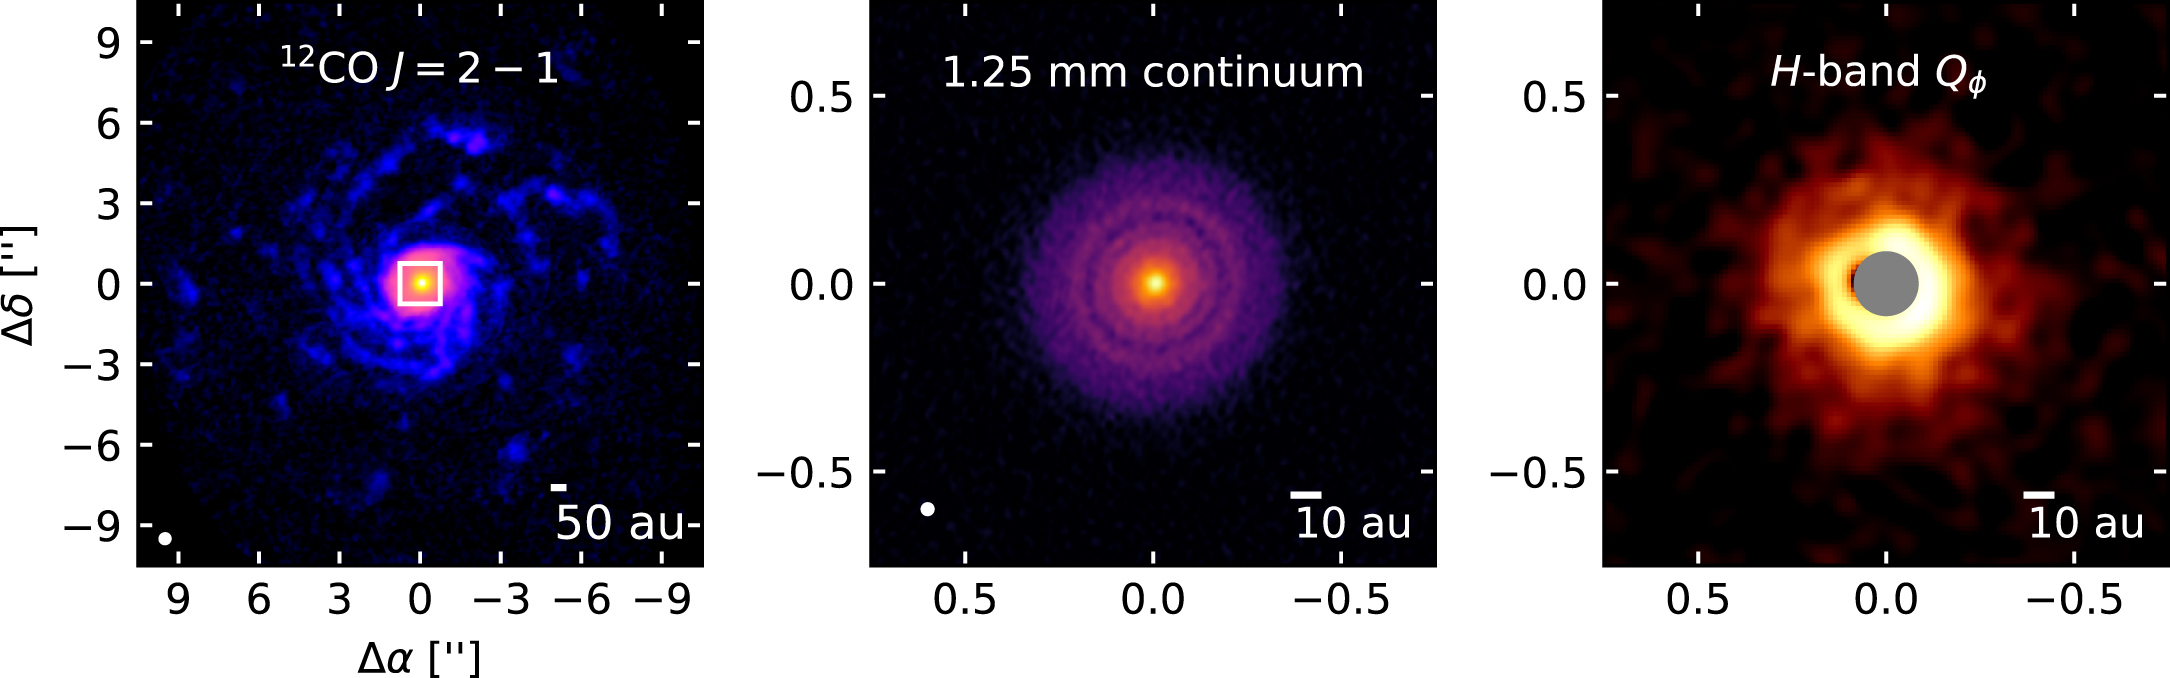
\includegraphics[width=\textwidth]{images/2.2.tracers.comparison/apjaba1e1f9_hr.jpg}
    \end{center}
    \caption{Comparison between observations of the RU Lup disc through the three main tracers.
    Image taken from ()}
\end{figure}


Direct observations of protoplanetary discs are of crucial importance for the detection and study of their morphology.
Properties of substructures, such as their shape and dimension, had, in fact, 
been proved to reveal key features of the disc itself and
of the objects that drive their formation. I am going to discuss how they are detected.

Due to their distance we can only look at their electromagnetic emission
and exploit the natural diversity of structures and properties. 
Three sources of light can be identified.

The first one is the radiation, usually of micrometric wavelength, emitted by the host star and scattered by dust grains.
This tracer is especially sensitive to the vertical structure 
of the disc allowing measures of the height and of the dust distribution along this direction.

The second tracer is the thermal continuum emission of solids, typically at millimetric wavelengths,
emitted in the optically thin regime which implies direct proportionality between the intensity of the radiation observed and the
mass density of the dust. Images of the disc thermal emission are, thus, of specific interest in the investigation of the solid grains.

On the contrary, the gas component eludes direct observations due to the nature of $H_2$ the dominant molecule.
This part of the disc can be detected thanks to spectral line emission of less abundant molecules 
that constitute the third category of observational primers. Measures made from these probes suffer from
the uncertainties in the molecular abundance of the revealed gases along with other problems
which make gas observation complex and uncertain.

In all of these cases the range of wavelengths probed is approximately $\SI{1}{\micro\m} - \SI{10}{\mm}$, hence going from infrared to radio waves.
As anticipated, protoplanetary discs have a diameter of about 100 a.u. at a typical distance of 100/150 pc. Therefore, telescopes need to acquire an angular
resolution under the arc second which is done using interferometric techniques. The leader observatory able to carry out this type of observations is the Atacama Large Millimiter Array (ALMA)
which is an array of 66 high precision antennas that can be moved to achieve different configurations. 
Other facilities that have given a significant contribution to the detection of protoplanetary discs are the Very Large Telescope (VLT), the W. M. Keck Observatory and the NASA
Hubble Space Telescope.

The images with the best resolution currently obtained are those of the DSHARP (Disk Substructures at High Angular Resolution Project) survey, $\sim 0.035$ arcsec, designed to examine properties
of small-scale substructures and inquire how they relate to the planet formation process. 

\section{Planet formation}

\begin{figure}
    \begin{center}
        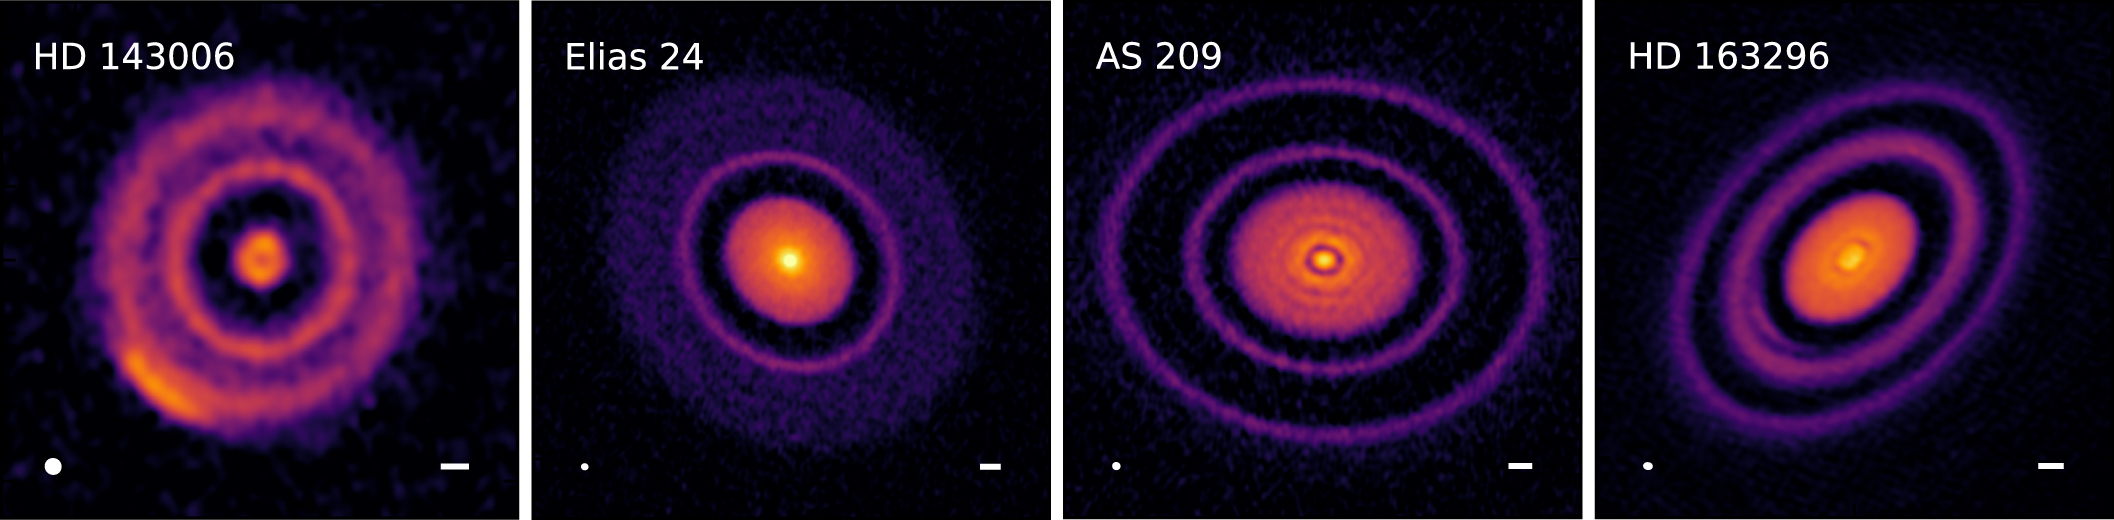
\includegraphics[width=\textwidth]{images/alma_pictures.jpg}
    \end{center}
    \caption{Examples of gaps and double gaps. 
    Observations of the dust continuum emission of some discs obtained from DSHARP.
    Image adapted from ()}
\end{figure}

\begin{comment}
Here I am going to discuss how planets are formed within these discs. 
I will explain: 

    — how they accrete their mass

    — the forces they experience and thus the radial drift

    — the substructures they form in the disc

    — typical mass values and their relation with substructures (qualitatively) 
\end{comment}

\begin{comment}
-introduction on the importance of planet formation and how ppd are the natural birthplace of planets
-how we go from debris to massive planets, mechanisms and the motion of the planet inside the disc
-substructures ad how they are related to the planet mass
\end{comment}

In 2006 the International Astronomical Union defined a planet as a celestial body in orbit around the sun with enough mass 
to reach a hydrostatic equilibrium (nearly round) shape and which has cleared the neighbourhood around its orbit. Outside the solar system 
the term planet indicates large bodies, in orbit around a star,
with a mass below the limit for thermonuclear fusion of deuterium, 
currently calculated to be 13 Jupyter masses for objects of sun metallicity. The lower mass threshold should instead be the same of that considered
for the solar system.

The study of extrasolar planets, often referred to as exoplanets, is of primary importance to make statistical studies of theories 
involving planets and their formation. Protoplanetary discs are the planets' birthplace. 
Different mechanisms of planet formation have been proposed and some parts of the theories are not completely
understood yet. 

The core accretion process is believed to be the origin of planets from the dust component of the disc. 
The process starts from the small dust grains which are well coupled with the gas.
The coupling makes them acquire low relative velocities that result in gentle collisions forming aggregates called, when a significant mass is reached, planetesimals.
While gradually accreting their mass, this aggregates settle towards the mid-plane and start to decouple from the gas experiencing a radial force 
which makes them spiral inwards toward the global maximum in the gas pressure. This motion is called radial drift and it is usually more effective for grains of sizes in the range 
1-10 mm.
The accretion process of planetesimals continues until the local dust population is depleted by radial migration or the collisions become destructive.

This process profoundly influences the morphology of the disc leaving us ways to detect and characterize newborn planets. 
Gaps, annular regions of dust or gas depletion, are the pivotal substructure generated from the interaction of the disc with young planets.
Links between their shape and planets features were found, which will be discussed in detail in the next chapter:
a measure of their width allows, for example, an indirect estimation of the planet mass.

\section{Gaps}

\begin{comment}
Here I am going to:

— explain how planets are not the only thing that generates gaps

— present the radial profile of a gap in dust and gas densities

— explain the differences between gap structures in gas and dust 

— explain how depth and width are defined
\end{comment}



Gaps are going to be the object of application for the investigative approach proposed in this thesis due
to their role in the detection of young planets.
For this reason I am going to throw some light on their properties.

They are one of the most common substructure observed in images of protoplanetary discs, and
planets are often the cause of their formation. However, other mechanisms were recognized to generate gaps
including magnetorotational instability turbulence, gravitational instabilities, condensation of molecular species along different snowlines,
large-scale vortices and self-induced dust pileups. The effective presence of a planet must hence be cautiously investigated and confirmed 
before inferring its features from the gaps properties. 

The figure 2.4 presents the radial profile of the gas and dust densities at a gap. Taking into exam 
the graph relative to the dust density, I am going to highlight some recurrent features:
at the core of the depletion zone, we can observe two minimums separated by a local maximum which usually coincides with the planet orbit.
Sometimes this maximum reaches values comparable with the density of the unperturbed disc, a substructure that can be identified as a double gap. 
The borders also presents local maximums. Gaps are usually wider and deeper in the dust rather than in the gas component where they could even
fail to form.

\begin{figure}
    \begin{center}
        %% Creator: Matplotlib, PGF backend
%%
%% To include the figure in your LaTeX document, write
%%   \input{<filename>.pgf}
%%
%% Make sure the required packages are loaded in your preamble
%%   \usepackage{pgf}
%%
%% Figures using additional raster images can only be included by \input if
%% they are in the same directory as the main LaTeX file. For loading figures
%% from other directories you can use the `import` package
%%   \usepackage{import}
%%
%% and then include the figures with
%%   \import{<path to file>}{<filename>.pgf}
%%
%% Matplotlib used the following preamble
%%
\begingroup%
\makeatletter%
\begin{pgfpicture}%
\pgfpathrectangle{\pgfpointorigin}{\pgfqpoint{5.900000in}{2.400000in}}%
\pgfusepath{use as bounding box, clip}%
\begin{pgfscope}%
\pgfsetbuttcap%
\pgfsetmiterjoin%
\pgfsetlinewidth{0.000000pt}%
\definecolor{currentstroke}{rgb}{1.000000,1.000000,1.000000}%
\pgfsetstrokecolor{currentstroke}%
\pgfsetstrokeopacity{0.000000}%
\pgfsetdash{}{0pt}%
\pgfpathmoveto{\pgfqpoint{0.000000in}{0.000000in}}%
\pgfpathlineto{\pgfqpoint{5.900000in}{0.000000in}}%
\pgfpathlineto{\pgfqpoint{5.900000in}{2.400000in}}%
\pgfpathlineto{\pgfqpoint{0.000000in}{2.400000in}}%
\pgfpathclose%
\pgfusepath{}%
\end{pgfscope}%
\begin{pgfscope}%
\pgfsetbuttcap%
\pgfsetmiterjoin%
\definecolor{currentfill}{rgb}{1.000000,1.000000,1.000000}%
\pgfsetfillcolor{currentfill}%
\pgfsetlinewidth{0.000000pt}%
\definecolor{currentstroke}{rgb}{0.000000,0.000000,0.000000}%
\pgfsetstrokecolor{currentstroke}%
\pgfsetstrokeopacity{0.000000}%
\pgfsetdash{}{0pt}%
\pgfpathmoveto{\pgfqpoint{0.664060in}{0.515123in}}%
\pgfpathlineto{\pgfqpoint{2.770833in}{0.515123in}}%
\pgfpathlineto{\pgfqpoint{2.770833in}{2.300000in}}%
\pgfpathlineto{\pgfqpoint{0.664060in}{2.300000in}}%
\pgfpathclose%
\pgfusepath{fill}%
\end{pgfscope}%
\begin{pgfscope}%
\pgfsetbuttcap%
\pgfsetroundjoin%
\definecolor{currentfill}{rgb}{0.000000,0.000000,0.000000}%
\pgfsetfillcolor{currentfill}%
\pgfsetlinewidth{0.803000pt}%
\definecolor{currentstroke}{rgb}{0.000000,0.000000,0.000000}%
\pgfsetstrokecolor{currentstroke}%
\pgfsetdash{}{0pt}%
\pgfsys@defobject{currentmarker}{\pgfqpoint{0.000000in}{-0.048611in}}{\pgfqpoint{0.000000in}{0.000000in}}{%
\pgfpathmoveto{\pgfqpoint{0.000000in}{0.000000in}}%
\pgfpathlineto{\pgfqpoint{0.000000in}{-0.048611in}}%
\pgfusepath{stroke,fill}%
}%
\begin{pgfscope}%
\pgfsys@transformshift{0.898146in}{0.515123in}%
\pgfsys@useobject{currentmarker}{}%
\end{pgfscope}%
\end{pgfscope}%
\begin{pgfscope}%
\definecolor{textcolor}{rgb}{0.000000,0.000000,0.000000}%
\pgfsetstrokecolor{textcolor}%
\pgfsetfillcolor{textcolor}%
\pgftext[x=0.898146in,y=0.417901in,,top]{\color{textcolor}\rmfamily\fontsize{10.000000}{12.000000}\selectfont \(\displaystyle {20}\)}%
\end{pgfscope}%
\begin{pgfscope}%
\pgfsetbuttcap%
\pgfsetroundjoin%
\definecolor{currentfill}{rgb}{0.000000,0.000000,0.000000}%
\pgfsetfillcolor{currentfill}%
\pgfsetlinewidth{0.803000pt}%
\definecolor{currentstroke}{rgb}{0.000000,0.000000,0.000000}%
\pgfsetstrokecolor{currentstroke}%
\pgfsetdash{}{0pt}%
\pgfsys@defobject{currentmarker}{\pgfqpoint{0.000000in}{-0.048611in}}{\pgfqpoint{0.000000in}{0.000000in}}{%
\pgfpathmoveto{\pgfqpoint{0.000000in}{0.000000in}}%
\pgfpathlineto{\pgfqpoint{0.000000in}{-0.048611in}}%
\pgfusepath{stroke,fill}%
}%
\begin{pgfscope}%
\pgfsys@transformshift{1.366318in}{0.515123in}%
\pgfsys@useobject{currentmarker}{}%
\end{pgfscope}%
\end{pgfscope}%
\begin{pgfscope}%
\definecolor{textcolor}{rgb}{0.000000,0.000000,0.000000}%
\pgfsetstrokecolor{textcolor}%
\pgfsetfillcolor{textcolor}%
\pgftext[x=1.366318in,y=0.417901in,,top]{\color{textcolor}\rmfamily\fontsize{10.000000}{12.000000}\selectfont \(\displaystyle {40}\)}%
\end{pgfscope}%
\begin{pgfscope}%
\pgfsetbuttcap%
\pgfsetroundjoin%
\definecolor{currentfill}{rgb}{0.000000,0.000000,0.000000}%
\pgfsetfillcolor{currentfill}%
\pgfsetlinewidth{0.803000pt}%
\definecolor{currentstroke}{rgb}{0.000000,0.000000,0.000000}%
\pgfsetstrokecolor{currentstroke}%
\pgfsetdash{}{0pt}%
\pgfsys@defobject{currentmarker}{\pgfqpoint{0.000000in}{-0.048611in}}{\pgfqpoint{0.000000in}{0.000000in}}{%
\pgfpathmoveto{\pgfqpoint{0.000000in}{0.000000in}}%
\pgfpathlineto{\pgfqpoint{0.000000in}{-0.048611in}}%
\pgfusepath{stroke,fill}%
}%
\begin{pgfscope}%
\pgfsys@transformshift{1.834489in}{0.515123in}%
\pgfsys@useobject{currentmarker}{}%
\end{pgfscope}%
\end{pgfscope}%
\begin{pgfscope}%
\definecolor{textcolor}{rgb}{0.000000,0.000000,0.000000}%
\pgfsetstrokecolor{textcolor}%
\pgfsetfillcolor{textcolor}%
\pgftext[x=1.834489in,y=0.417901in,,top]{\color{textcolor}\rmfamily\fontsize{10.000000}{12.000000}\selectfont \(\displaystyle {60}\)}%
\end{pgfscope}%
\begin{pgfscope}%
\pgfsetbuttcap%
\pgfsetroundjoin%
\definecolor{currentfill}{rgb}{0.000000,0.000000,0.000000}%
\pgfsetfillcolor{currentfill}%
\pgfsetlinewidth{0.803000pt}%
\definecolor{currentstroke}{rgb}{0.000000,0.000000,0.000000}%
\pgfsetstrokecolor{currentstroke}%
\pgfsetdash{}{0pt}%
\pgfsys@defobject{currentmarker}{\pgfqpoint{0.000000in}{-0.048611in}}{\pgfqpoint{0.000000in}{0.000000in}}{%
\pgfpathmoveto{\pgfqpoint{0.000000in}{0.000000in}}%
\pgfpathlineto{\pgfqpoint{0.000000in}{-0.048611in}}%
\pgfusepath{stroke,fill}%
}%
\begin{pgfscope}%
\pgfsys@transformshift{2.302661in}{0.515123in}%
\pgfsys@useobject{currentmarker}{}%
\end{pgfscope}%
\end{pgfscope}%
\begin{pgfscope}%
\definecolor{textcolor}{rgb}{0.000000,0.000000,0.000000}%
\pgfsetstrokecolor{textcolor}%
\pgfsetfillcolor{textcolor}%
\pgftext[x=2.302661in,y=0.417901in,,top]{\color{textcolor}\rmfamily\fontsize{10.000000}{12.000000}\selectfont \(\displaystyle {80}\)}%
\end{pgfscope}%
\begin{pgfscope}%
\pgfsetbuttcap%
\pgfsetroundjoin%
\definecolor{currentfill}{rgb}{0.000000,0.000000,0.000000}%
\pgfsetfillcolor{currentfill}%
\pgfsetlinewidth{0.803000pt}%
\definecolor{currentstroke}{rgb}{0.000000,0.000000,0.000000}%
\pgfsetstrokecolor{currentstroke}%
\pgfsetdash{}{0pt}%
\pgfsys@defobject{currentmarker}{\pgfqpoint{0.000000in}{-0.048611in}}{\pgfqpoint{0.000000in}{0.000000in}}{%
\pgfpathmoveto{\pgfqpoint{0.000000in}{0.000000in}}%
\pgfpathlineto{\pgfqpoint{0.000000in}{-0.048611in}}%
\pgfusepath{stroke,fill}%
}%
\begin{pgfscope}%
\pgfsys@transformshift{2.770833in}{0.515123in}%
\pgfsys@useobject{currentmarker}{}%
\end{pgfscope}%
\end{pgfscope}%
\begin{pgfscope}%
\definecolor{textcolor}{rgb}{0.000000,0.000000,0.000000}%
\pgfsetstrokecolor{textcolor}%
\pgfsetfillcolor{textcolor}%
\pgftext[x=2.770833in,y=0.417901in,,top]{\color{textcolor}\rmfamily\fontsize{10.000000}{12.000000}\selectfont \(\displaystyle {100}\)}%
\end{pgfscope}%
\begin{pgfscope}%
\definecolor{textcolor}{rgb}{0.000000,0.000000,0.000000}%
\pgfsetstrokecolor{textcolor}%
\pgfsetfillcolor{textcolor}%
\pgftext[x=1.717446in,y=0.238889in,,top]{\color{textcolor}\rmfamily\fontsize{10.000000}{12.000000}\selectfont Radius [au]}%
\end{pgfscope}%
\begin{pgfscope}%
\pgfsetbuttcap%
\pgfsetroundjoin%
\definecolor{currentfill}{rgb}{0.000000,0.000000,0.000000}%
\pgfsetfillcolor{currentfill}%
\pgfsetlinewidth{0.803000pt}%
\definecolor{currentstroke}{rgb}{0.000000,0.000000,0.000000}%
\pgfsetstrokecolor{currentstroke}%
\pgfsetdash{}{0pt}%
\pgfsys@defobject{currentmarker}{\pgfqpoint{-0.048611in}{0.000000in}}{\pgfqpoint{-0.000000in}{0.000000in}}{%
\pgfpathmoveto{\pgfqpoint{-0.000000in}{0.000000in}}%
\pgfpathlineto{\pgfqpoint{-0.048611in}{0.000000in}}%
\pgfusepath{stroke,fill}%
}%
\begin{pgfscope}%
\pgfsys@transformshift{0.664060in}{1.256764in}%
\pgfsys@useobject{currentmarker}{}%
\end{pgfscope}%
\end{pgfscope}%
\begin{pgfscope}%
\definecolor{textcolor}{rgb}{0.000000,0.000000,0.000000}%
\pgfsetstrokecolor{textcolor}%
\pgfsetfillcolor{textcolor}%
\pgftext[x=0.310278in, y=1.208539in, left, base]{\color{textcolor}\rmfamily\fontsize{10.000000}{12.000000}\selectfont \(\displaystyle {10^{22}}\)}%
\end{pgfscope}%
\begin{pgfscope}%
\pgfsetbuttcap%
\pgfsetroundjoin%
\definecolor{currentfill}{rgb}{0.000000,0.000000,0.000000}%
\pgfsetfillcolor{currentfill}%
\pgfsetlinewidth{0.803000pt}%
\definecolor{currentstroke}{rgb}{0.000000,0.000000,0.000000}%
\pgfsetstrokecolor{currentstroke}%
\pgfsetdash{}{0pt}%
\pgfsys@defobject{currentmarker}{\pgfqpoint{-0.048611in}{0.000000in}}{\pgfqpoint{-0.000000in}{0.000000in}}{%
\pgfpathmoveto{\pgfqpoint{-0.000000in}{0.000000in}}%
\pgfpathlineto{\pgfqpoint{-0.048611in}{0.000000in}}%
\pgfusepath{stroke,fill}%
}%
\begin{pgfscope}%
\pgfsys@transformshift{0.664060in}{2.234579in}%
\pgfsys@useobject{currentmarker}{}%
\end{pgfscope}%
\end{pgfscope}%
\begin{pgfscope}%
\definecolor{textcolor}{rgb}{0.000000,0.000000,0.000000}%
\pgfsetstrokecolor{textcolor}%
\pgfsetfillcolor{textcolor}%
\pgftext[x=0.310278in, y=2.186353in, left, base]{\color{textcolor}\rmfamily\fontsize{10.000000}{12.000000}\selectfont \(\displaystyle {10^{23}}\)}%
\end{pgfscope}%
\begin{pgfscope}%
\pgfsetbuttcap%
\pgfsetroundjoin%
\definecolor{currentfill}{rgb}{0.000000,0.000000,0.000000}%
\pgfsetfillcolor{currentfill}%
\pgfsetlinewidth{0.602250pt}%
\definecolor{currentstroke}{rgb}{0.000000,0.000000,0.000000}%
\pgfsetstrokecolor{currentstroke}%
\pgfsetdash{}{0pt}%
\pgfsys@defobject{currentmarker}{\pgfqpoint{-0.027778in}{0.000000in}}{\pgfqpoint{-0.000000in}{0.000000in}}{%
\pgfpathmoveto{\pgfqpoint{-0.000000in}{0.000000in}}%
\pgfpathlineto{\pgfqpoint{-0.027778in}{0.000000in}}%
\pgfusepath{stroke,fill}%
}%
\begin{pgfscope}%
\pgfsys@transformshift{0.664060in}{0.573301in}%
\pgfsys@useobject{currentmarker}{}%
\end{pgfscope}%
\end{pgfscope}%
\begin{pgfscope}%
\pgfsetbuttcap%
\pgfsetroundjoin%
\definecolor{currentfill}{rgb}{0.000000,0.000000,0.000000}%
\pgfsetfillcolor{currentfill}%
\pgfsetlinewidth{0.602250pt}%
\definecolor{currentstroke}{rgb}{0.000000,0.000000,0.000000}%
\pgfsetstrokecolor{currentstroke}%
\pgfsetdash{}{0pt}%
\pgfsys@defobject{currentmarker}{\pgfqpoint{-0.027778in}{0.000000in}}{\pgfqpoint{-0.000000in}{0.000000in}}{%
\pgfpathmoveto{\pgfqpoint{-0.000000in}{0.000000in}}%
\pgfpathlineto{\pgfqpoint{-0.027778in}{0.000000in}}%
\pgfusepath{stroke,fill}%
}%
\begin{pgfscope}%
\pgfsys@transformshift{0.664060in}{0.745485in}%
\pgfsys@useobject{currentmarker}{}%
\end{pgfscope}%
\end{pgfscope}%
\begin{pgfscope}%
\pgfsetbuttcap%
\pgfsetroundjoin%
\definecolor{currentfill}{rgb}{0.000000,0.000000,0.000000}%
\pgfsetfillcolor{currentfill}%
\pgfsetlinewidth{0.602250pt}%
\definecolor{currentstroke}{rgb}{0.000000,0.000000,0.000000}%
\pgfsetstrokecolor{currentstroke}%
\pgfsetdash{}{0pt}%
\pgfsys@defobject{currentmarker}{\pgfqpoint{-0.027778in}{0.000000in}}{\pgfqpoint{-0.000000in}{0.000000in}}{%
\pgfpathmoveto{\pgfqpoint{-0.000000in}{0.000000in}}%
\pgfpathlineto{\pgfqpoint{-0.027778in}{0.000000in}}%
\pgfusepath{stroke,fill}%
}%
\begin{pgfscope}%
\pgfsys@transformshift{0.664060in}{0.867652in}%
\pgfsys@useobject{currentmarker}{}%
\end{pgfscope}%
\end{pgfscope}%
\begin{pgfscope}%
\pgfsetbuttcap%
\pgfsetroundjoin%
\definecolor{currentfill}{rgb}{0.000000,0.000000,0.000000}%
\pgfsetfillcolor{currentfill}%
\pgfsetlinewidth{0.602250pt}%
\definecolor{currentstroke}{rgb}{0.000000,0.000000,0.000000}%
\pgfsetstrokecolor{currentstroke}%
\pgfsetdash{}{0pt}%
\pgfsys@defobject{currentmarker}{\pgfqpoint{-0.027778in}{0.000000in}}{\pgfqpoint{-0.000000in}{0.000000in}}{%
\pgfpathmoveto{\pgfqpoint{-0.000000in}{0.000000in}}%
\pgfpathlineto{\pgfqpoint{-0.027778in}{0.000000in}}%
\pgfusepath{stroke,fill}%
}%
\begin{pgfscope}%
\pgfsys@transformshift{0.664060in}{0.962412in}%
\pgfsys@useobject{currentmarker}{}%
\end{pgfscope}%
\end{pgfscope}%
\begin{pgfscope}%
\pgfsetbuttcap%
\pgfsetroundjoin%
\definecolor{currentfill}{rgb}{0.000000,0.000000,0.000000}%
\pgfsetfillcolor{currentfill}%
\pgfsetlinewidth{0.602250pt}%
\definecolor{currentstroke}{rgb}{0.000000,0.000000,0.000000}%
\pgfsetstrokecolor{currentstroke}%
\pgfsetdash{}{0pt}%
\pgfsys@defobject{currentmarker}{\pgfqpoint{-0.027778in}{0.000000in}}{\pgfqpoint{-0.000000in}{0.000000in}}{%
\pgfpathmoveto{\pgfqpoint{-0.000000in}{0.000000in}}%
\pgfpathlineto{\pgfqpoint{-0.027778in}{0.000000in}}%
\pgfusepath{stroke,fill}%
}%
\begin{pgfscope}%
\pgfsys@transformshift{0.664060in}{1.039837in}%
\pgfsys@useobject{currentmarker}{}%
\end{pgfscope}%
\end{pgfscope}%
\begin{pgfscope}%
\pgfsetbuttcap%
\pgfsetroundjoin%
\definecolor{currentfill}{rgb}{0.000000,0.000000,0.000000}%
\pgfsetfillcolor{currentfill}%
\pgfsetlinewidth{0.602250pt}%
\definecolor{currentstroke}{rgb}{0.000000,0.000000,0.000000}%
\pgfsetstrokecolor{currentstroke}%
\pgfsetdash{}{0pt}%
\pgfsys@defobject{currentmarker}{\pgfqpoint{-0.027778in}{0.000000in}}{\pgfqpoint{-0.000000in}{0.000000in}}{%
\pgfpathmoveto{\pgfqpoint{-0.000000in}{0.000000in}}%
\pgfpathlineto{\pgfqpoint{-0.027778in}{0.000000in}}%
\pgfusepath{stroke,fill}%
}%
\begin{pgfscope}%
\pgfsys@transformshift{0.664060in}{1.105299in}%
\pgfsys@useobject{currentmarker}{}%
\end{pgfscope}%
\end{pgfscope}%
\begin{pgfscope}%
\pgfsetbuttcap%
\pgfsetroundjoin%
\definecolor{currentfill}{rgb}{0.000000,0.000000,0.000000}%
\pgfsetfillcolor{currentfill}%
\pgfsetlinewidth{0.602250pt}%
\definecolor{currentstroke}{rgb}{0.000000,0.000000,0.000000}%
\pgfsetstrokecolor{currentstroke}%
\pgfsetdash{}{0pt}%
\pgfsys@defobject{currentmarker}{\pgfqpoint{-0.027778in}{0.000000in}}{\pgfqpoint{-0.000000in}{0.000000in}}{%
\pgfpathmoveto{\pgfqpoint{-0.000000in}{0.000000in}}%
\pgfpathlineto{\pgfqpoint{-0.027778in}{0.000000in}}%
\pgfusepath{stroke,fill}%
}%
\begin{pgfscope}%
\pgfsys@transformshift{0.664060in}{1.162004in}%
\pgfsys@useobject{currentmarker}{}%
\end{pgfscope}%
\end{pgfscope}%
\begin{pgfscope}%
\pgfsetbuttcap%
\pgfsetroundjoin%
\definecolor{currentfill}{rgb}{0.000000,0.000000,0.000000}%
\pgfsetfillcolor{currentfill}%
\pgfsetlinewidth{0.602250pt}%
\definecolor{currentstroke}{rgb}{0.000000,0.000000,0.000000}%
\pgfsetstrokecolor{currentstroke}%
\pgfsetdash{}{0pt}%
\pgfsys@defobject{currentmarker}{\pgfqpoint{-0.027778in}{0.000000in}}{\pgfqpoint{-0.000000in}{0.000000in}}{%
\pgfpathmoveto{\pgfqpoint{-0.000000in}{0.000000in}}%
\pgfpathlineto{\pgfqpoint{-0.027778in}{0.000000in}}%
\pgfusepath{stroke,fill}%
}%
\begin{pgfscope}%
\pgfsys@transformshift{0.664060in}{1.212022in}%
\pgfsys@useobject{currentmarker}{}%
\end{pgfscope}%
\end{pgfscope}%
\begin{pgfscope}%
\pgfsetbuttcap%
\pgfsetroundjoin%
\definecolor{currentfill}{rgb}{0.000000,0.000000,0.000000}%
\pgfsetfillcolor{currentfill}%
\pgfsetlinewidth{0.602250pt}%
\definecolor{currentstroke}{rgb}{0.000000,0.000000,0.000000}%
\pgfsetstrokecolor{currentstroke}%
\pgfsetdash{}{0pt}%
\pgfsys@defobject{currentmarker}{\pgfqpoint{-0.027778in}{0.000000in}}{\pgfqpoint{-0.000000in}{0.000000in}}{%
\pgfpathmoveto{\pgfqpoint{-0.000000in}{0.000000in}}%
\pgfpathlineto{\pgfqpoint{-0.027778in}{0.000000in}}%
\pgfusepath{stroke,fill}%
}%
\begin{pgfscope}%
\pgfsys@transformshift{0.664060in}{1.551115in}%
\pgfsys@useobject{currentmarker}{}%
\end{pgfscope}%
\end{pgfscope}%
\begin{pgfscope}%
\pgfsetbuttcap%
\pgfsetroundjoin%
\definecolor{currentfill}{rgb}{0.000000,0.000000,0.000000}%
\pgfsetfillcolor{currentfill}%
\pgfsetlinewidth{0.602250pt}%
\definecolor{currentstroke}{rgb}{0.000000,0.000000,0.000000}%
\pgfsetstrokecolor{currentstroke}%
\pgfsetdash{}{0pt}%
\pgfsys@defobject{currentmarker}{\pgfqpoint{-0.027778in}{0.000000in}}{\pgfqpoint{-0.000000in}{0.000000in}}{%
\pgfpathmoveto{\pgfqpoint{-0.000000in}{0.000000in}}%
\pgfpathlineto{\pgfqpoint{-0.027778in}{0.000000in}}%
\pgfusepath{stroke,fill}%
}%
\begin{pgfscope}%
\pgfsys@transformshift{0.664060in}{1.723300in}%
\pgfsys@useobject{currentmarker}{}%
\end{pgfscope}%
\end{pgfscope}%
\begin{pgfscope}%
\pgfsetbuttcap%
\pgfsetroundjoin%
\definecolor{currentfill}{rgb}{0.000000,0.000000,0.000000}%
\pgfsetfillcolor{currentfill}%
\pgfsetlinewidth{0.602250pt}%
\definecolor{currentstroke}{rgb}{0.000000,0.000000,0.000000}%
\pgfsetstrokecolor{currentstroke}%
\pgfsetdash{}{0pt}%
\pgfsys@defobject{currentmarker}{\pgfqpoint{-0.027778in}{0.000000in}}{\pgfqpoint{-0.000000in}{0.000000in}}{%
\pgfpathmoveto{\pgfqpoint{-0.000000in}{0.000000in}}%
\pgfpathlineto{\pgfqpoint{-0.027778in}{0.000000in}}%
\pgfusepath{stroke,fill}%
}%
\begin{pgfscope}%
\pgfsys@transformshift{0.664060in}{1.845467in}%
\pgfsys@useobject{currentmarker}{}%
\end{pgfscope}%
\end{pgfscope}%
\begin{pgfscope}%
\pgfsetbuttcap%
\pgfsetroundjoin%
\definecolor{currentfill}{rgb}{0.000000,0.000000,0.000000}%
\pgfsetfillcolor{currentfill}%
\pgfsetlinewidth{0.602250pt}%
\definecolor{currentstroke}{rgb}{0.000000,0.000000,0.000000}%
\pgfsetstrokecolor{currentstroke}%
\pgfsetdash{}{0pt}%
\pgfsys@defobject{currentmarker}{\pgfqpoint{-0.027778in}{0.000000in}}{\pgfqpoint{-0.000000in}{0.000000in}}{%
\pgfpathmoveto{\pgfqpoint{-0.000000in}{0.000000in}}%
\pgfpathlineto{\pgfqpoint{-0.027778in}{0.000000in}}%
\pgfusepath{stroke,fill}%
}%
\begin{pgfscope}%
\pgfsys@transformshift{0.664060in}{1.940227in}%
\pgfsys@useobject{currentmarker}{}%
\end{pgfscope}%
\end{pgfscope}%
\begin{pgfscope}%
\pgfsetbuttcap%
\pgfsetroundjoin%
\definecolor{currentfill}{rgb}{0.000000,0.000000,0.000000}%
\pgfsetfillcolor{currentfill}%
\pgfsetlinewidth{0.602250pt}%
\definecolor{currentstroke}{rgb}{0.000000,0.000000,0.000000}%
\pgfsetstrokecolor{currentstroke}%
\pgfsetdash{}{0pt}%
\pgfsys@defobject{currentmarker}{\pgfqpoint{-0.027778in}{0.000000in}}{\pgfqpoint{-0.000000in}{0.000000in}}{%
\pgfpathmoveto{\pgfqpoint{-0.000000in}{0.000000in}}%
\pgfpathlineto{\pgfqpoint{-0.027778in}{0.000000in}}%
\pgfusepath{stroke,fill}%
}%
\begin{pgfscope}%
\pgfsys@transformshift{0.664060in}{2.017652in}%
\pgfsys@useobject{currentmarker}{}%
\end{pgfscope}%
\end{pgfscope}%
\begin{pgfscope}%
\pgfsetbuttcap%
\pgfsetroundjoin%
\definecolor{currentfill}{rgb}{0.000000,0.000000,0.000000}%
\pgfsetfillcolor{currentfill}%
\pgfsetlinewidth{0.602250pt}%
\definecolor{currentstroke}{rgb}{0.000000,0.000000,0.000000}%
\pgfsetstrokecolor{currentstroke}%
\pgfsetdash{}{0pt}%
\pgfsys@defobject{currentmarker}{\pgfqpoint{-0.027778in}{0.000000in}}{\pgfqpoint{-0.000000in}{0.000000in}}{%
\pgfpathmoveto{\pgfqpoint{-0.000000in}{0.000000in}}%
\pgfpathlineto{\pgfqpoint{-0.027778in}{0.000000in}}%
\pgfusepath{stroke,fill}%
}%
\begin{pgfscope}%
\pgfsys@transformshift{0.664060in}{2.083113in}%
\pgfsys@useobject{currentmarker}{}%
\end{pgfscope}%
\end{pgfscope}%
\begin{pgfscope}%
\pgfsetbuttcap%
\pgfsetroundjoin%
\definecolor{currentfill}{rgb}{0.000000,0.000000,0.000000}%
\pgfsetfillcolor{currentfill}%
\pgfsetlinewidth{0.602250pt}%
\definecolor{currentstroke}{rgb}{0.000000,0.000000,0.000000}%
\pgfsetstrokecolor{currentstroke}%
\pgfsetdash{}{0pt}%
\pgfsys@defobject{currentmarker}{\pgfqpoint{-0.027778in}{0.000000in}}{\pgfqpoint{-0.000000in}{0.000000in}}{%
\pgfpathmoveto{\pgfqpoint{-0.000000in}{0.000000in}}%
\pgfpathlineto{\pgfqpoint{-0.027778in}{0.000000in}}%
\pgfusepath{stroke,fill}%
}%
\begin{pgfscope}%
\pgfsys@transformshift{0.664060in}{2.139819in}%
\pgfsys@useobject{currentmarker}{}%
\end{pgfscope}%
\end{pgfscope}%
\begin{pgfscope}%
\pgfsetbuttcap%
\pgfsetroundjoin%
\definecolor{currentfill}{rgb}{0.000000,0.000000,0.000000}%
\pgfsetfillcolor{currentfill}%
\pgfsetlinewidth{0.602250pt}%
\definecolor{currentstroke}{rgb}{0.000000,0.000000,0.000000}%
\pgfsetstrokecolor{currentstroke}%
\pgfsetdash{}{0pt}%
\pgfsys@defobject{currentmarker}{\pgfqpoint{-0.027778in}{0.000000in}}{\pgfqpoint{-0.000000in}{0.000000in}}{%
\pgfpathmoveto{\pgfqpoint{-0.000000in}{0.000000in}}%
\pgfpathlineto{\pgfqpoint{-0.027778in}{0.000000in}}%
\pgfusepath{stroke,fill}%
}%
\begin{pgfscope}%
\pgfsys@transformshift{0.664060in}{2.189836in}%
\pgfsys@useobject{currentmarker}{}%
\end{pgfscope}%
\end{pgfscope}%
\begin{pgfscope}%
\definecolor{textcolor}{rgb}{0.000000,0.000000,0.000000}%
\pgfsetstrokecolor{textcolor}%
\pgfsetfillcolor{textcolor}%
\pgftext[x=0.254723in,y=1.407562in,,bottom,rotate=90.000000]{\color{textcolor}\rmfamily\fontsize{10.000000}{12.000000}\selectfont Gas surface density [g/cm\(\displaystyle {}^2\)]}%
\end{pgfscope}%
\begin{pgfscope}%
\pgfpathrectangle{\pgfqpoint{0.664060in}{0.515123in}}{\pgfqpoint{2.106773in}{1.784877in}}%
\pgfusepath{clip}%
\pgfsetrectcap%
\pgfsetroundjoin%
\pgfsetlinewidth{1.505625pt}%
\definecolor{currentstroke}{rgb}{0.000000,0.000000,0.000000}%
\pgfsetstrokecolor{currentstroke}%
\pgfsetdash{}{0pt}%
\pgfpathmoveto{\pgfqpoint{0.685128in}{0.596254in}}%
\pgfpathlineto{\pgfqpoint{0.727263in}{0.791385in}}%
\pgfpathlineto{\pgfqpoint{0.769399in}{0.991377in}}%
\pgfpathlineto{\pgfqpoint{0.811534in}{1.099352in}}%
\pgfpathlineto{\pgfqpoint{0.853670in}{1.198607in}}%
\pgfpathlineto{\pgfqpoint{0.895805in}{1.283217in}}%
\pgfpathlineto{\pgfqpoint{0.937940in}{1.312318in}}%
\pgfpathlineto{\pgfqpoint{0.980076in}{1.310786in}}%
\pgfpathlineto{\pgfqpoint{1.022211in}{1.285997in}}%
\pgfpathlineto{\pgfqpoint{1.064347in}{1.263406in}}%
\pgfpathlineto{\pgfqpoint{1.106482in}{1.209090in}}%
\pgfpathlineto{\pgfqpoint{1.148618in}{1.244733in}}%
\pgfpathlineto{\pgfqpoint{1.190753in}{1.246424in}}%
\pgfpathlineto{\pgfqpoint{1.232889in}{1.266903in}}%
\pgfpathlineto{\pgfqpoint{1.275024in}{1.341589in}}%
\pgfpathlineto{\pgfqpoint{1.317160in}{1.398735in}}%
\pgfpathlineto{\pgfqpoint{1.359295in}{1.515343in}}%
\pgfpathlineto{\pgfqpoint{1.401431in}{1.632825in}}%
\pgfpathlineto{\pgfqpoint{1.443566in}{1.743037in}}%
\pgfpathlineto{\pgfqpoint{1.485701in}{1.840860in}}%
\pgfpathlineto{\pgfqpoint{1.527837in}{1.920404in}}%
\pgfpathlineto{\pgfqpoint{1.569972in}{1.997211in}}%
\pgfpathlineto{\pgfqpoint{1.612108in}{2.039963in}}%
\pgfpathlineto{\pgfqpoint{1.654243in}{2.085571in}}%
\pgfpathlineto{\pgfqpoint{1.696379in}{2.116816in}}%
\pgfpathlineto{\pgfqpoint{1.738514in}{2.147741in}}%
\pgfpathlineto{\pgfqpoint{1.780650in}{2.162103in}}%
\pgfpathlineto{\pgfqpoint{1.822785in}{2.181360in}}%
\pgfpathlineto{\pgfqpoint{1.864921in}{2.193839in}}%
\pgfpathlineto{\pgfqpoint{1.907056in}{2.201977in}}%
\pgfpathlineto{\pgfqpoint{1.949192in}{2.210676in}}%
\pgfpathlineto{\pgfqpoint{1.991327in}{2.215647in}}%
\pgfpathlineto{\pgfqpoint{2.033462in}{2.218869in}}%
\pgfpathlineto{\pgfqpoint{2.075598in}{2.212724in}}%
\pgfpathlineto{\pgfqpoint{2.117733in}{2.212131in}}%
\pgfpathlineto{\pgfqpoint{2.159869in}{2.206142in}}%
\pgfpathlineto{\pgfqpoint{2.202004in}{2.198589in}}%
\pgfpathlineto{\pgfqpoint{2.244140in}{2.194196in}}%
\pgfpathlineto{\pgfqpoint{2.286275in}{2.177611in}}%
\pgfpathlineto{\pgfqpoint{2.328411in}{2.166091in}}%
\pgfpathlineto{\pgfqpoint{2.370546in}{2.156298in}}%
\pgfpathlineto{\pgfqpoint{2.412682in}{2.141838in}}%
\pgfpathlineto{\pgfqpoint{2.454817in}{2.127341in}}%
\pgfpathlineto{\pgfqpoint{2.496952in}{2.109115in}}%
\pgfpathlineto{\pgfqpoint{2.539088in}{2.093769in}}%
\pgfpathlineto{\pgfqpoint{2.581223in}{2.081376in}}%
\pgfpathlineto{\pgfqpoint{2.623359in}{2.062379in}}%
\pgfpathlineto{\pgfqpoint{2.665494in}{2.045513in}}%
\pgfpathlineto{\pgfqpoint{2.707630in}{2.023628in}}%
\pgfpathlineto{\pgfqpoint{2.749765in}{2.006007in}}%
\pgfusepath{stroke}%
\end{pgfscope}%
\begin{pgfscope}%
\pgfsetrectcap%
\pgfsetmiterjoin%
\pgfsetlinewidth{0.803000pt}%
\definecolor{currentstroke}{rgb}{0.000000,0.000000,0.000000}%
\pgfsetstrokecolor{currentstroke}%
\pgfsetdash{}{0pt}%
\pgfpathmoveto{\pgfqpoint{0.664060in}{0.515123in}}%
\pgfpathlineto{\pgfqpoint{0.664060in}{2.300000in}}%
\pgfusepath{stroke}%
\end{pgfscope}%
\begin{pgfscope}%
\pgfsetrectcap%
\pgfsetmiterjoin%
\pgfsetlinewidth{0.803000pt}%
\definecolor{currentstroke}{rgb}{0.000000,0.000000,0.000000}%
\pgfsetstrokecolor{currentstroke}%
\pgfsetdash{}{0pt}%
\pgfpathmoveto{\pgfqpoint{2.770833in}{0.515123in}}%
\pgfpathlineto{\pgfqpoint{2.770833in}{2.300000in}}%
\pgfusepath{stroke}%
\end{pgfscope}%
\begin{pgfscope}%
\pgfsetrectcap%
\pgfsetmiterjoin%
\pgfsetlinewidth{0.803000pt}%
\definecolor{currentstroke}{rgb}{0.000000,0.000000,0.000000}%
\pgfsetstrokecolor{currentstroke}%
\pgfsetdash{}{0pt}%
\pgfpathmoveto{\pgfqpoint{0.664060in}{0.515123in}}%
\pgfpathlineto{\pgfqpoint{2.770833in}{0.515123in}}%
\pgfusepath{stroke}%
\end{pgfscope}%
\begin{pgfscope}%
\pgfsetrectcap%
\pgfsetmiterjoin%
\pgfsetlinewidth{0.803000pt}%
\definecolor{currentstroke}{rgb}{0.000000,0.000000,0.000000}%
\pgfsetstrokecolor{currentstroke}%
\pgfsetdash{}{0pt}%
\pgfpathmoveto{\pgfqpoint{0.664060in}{2.300000in}}%
\pgfpathlineto{\pgfqpoint{2.770833in}{2.300000in}}%
\pgfusepath{stroke}%
\end{pgfscope}%
\begin{pgfscope}%
\pgfsetbuttcap%
\pgfsetmiterjoin%
\definecolor{currentfill}{rgb}{1.000000,1.000000,1.000000}%
\pgfsetfillcolor{currentfill}%
\pgfsetlinewidth{0.000000pt}%
\definecolor{currentstroke}{rgb}{0.000000,0.000000,0.000000}%
\pgfsetstrokecolor{currentstroke}%
\pgfsetstrokeopacity{0.000000}%
\pgfsetdash{}{0pt}%
\pgfpathmoveto{\pgfqpoint{3.589060in}{0.515123in}}%
\pgfpathlineto{\pgfqpoint{5.695833in}{0.515123in}}%
\pgfpathlineto{\pgfqpoint{5.695833in}{2.300000in}}%
\pgfpathlineto{\pgfqpoint{3.589060in}{2.300000in}}%
\pgfpathclose%
\pgfusepath{fill}%
\end{pgfscope}%
\begin{pgfscope}%
\pgfsetbuttcap%
\pgfsetroundjoin%
\definecolor{currentfill}{rgb}{0.000000,0.000000,0.000000}%
\pgfsetfillcolor{currentfill}%
\pgfsetlinewidth{0.803000pt}%
\definecolor{currentstroke}{rgb}{0.000000,0.000000,0.000000}%
\pgfsetstrokecolor{currentstroke}%
\pgfsetdash{}{0pt}%
\pgfsys@defobject{currentmarker}{\pgfqpoint{0.000000in}{-0.048611in}}{\pgfqpoint{0.000000in}{0.000000in}}{%
\pgfpathmoveto{\pgfqpoint{0.000000in}{0.000000in}}%
\pgfpathlineto{\pgfqpoint{0.000000in}{-0.048611in}}%
\pgfusepath{stroke,fill}%
}%
\begin{pgfscope}%
\pgfsys@transformshift{3.823146in}{0.515123in}%
\pgfsys@useobject{currentmarker}{}%
\end{pgfscope}%
\end{pgfscope}%
\begin{pgfscope}%
\definecolor{textcolor}{rgb}{0.000000,0.000000,0.000000}%
\pgfsetstrokecolor{textcolor}%
\pgfsetfillcolor{textcolor}%
\pgftext[x=3.823146in,y=0.417901in,,top]{\color{textcolor}\rmfamily\fontsize{10.000000}{12.000000}\selectfont \(\displaystyle {20}\)}%
\end{pgfscope}%
\begin{pgfscope}%
\pgfsetbuttcap%
\pgfsetroundjoin%
\definecolor{currentfill}{rgb}{0.000000,0.000000,0.000000}%
\pgfsetfillcolor{currentfill}%
\pgfsetlinewidth{0.803000pt}%
\definecolor{currentstroke}{rgb}{0.000000,0.000000,0.000000}%
\pgfsetstrokecolor{currentstroke}%
\pgfsetdash{}{0pt}%
\pgfsys@defobject{currentmarker}{\pgfqpoint{0.000000in}{-0.048611in}}{\pgfqpoint{0.000000in}{0.000000in}}{%
\pgfpathmoveto{\pgfqpoint{0.000000in}{0.000000in}}%
\pgfpathlineto{\pgfqpoint{0.000000in}{-0.048611in}}%
\pgfusepath{stroke,fill}%
}%
\begin{pgfscope}%
\pgfsys@transformshift{4.291318in}{0.515123in}%
\pgfsys@useobject{currentmarker}{}%
\end{pgfscope}%
\end{pgfscope}%
\begin{pgfscope}%
\definecolor{textcolor}{rgb}{0.000000,0.000000,0.000000}%
\pgfsetstrokecolor{textcolor}%
\pgfsetfillcolor{textcolor}%
\pgftext[x=4.291318in,y=0.417901in,,top]{\color{textcolor}\rmfamily\fontsize{10.000000}{12.000000}\selectfont \(\displaystyle {40}\)}%
\end{pgfscope}%
\begin{pgfscope}%
\pgfsetbuttcap%
\pgfsetroundjoin%
\definecolor{currentfill}{rgb}{0.000000,0.000000,0.000000}%
\pgfsetfillcolor{currentfill}%
\pgfsetlinewidth{0.803000pt}%
\definecolor{currentstroke}{rgb}{0.000000,0.000000,0.000000}%
\pgfsetstrokecolor{currentstroke}%
\pgfsetdash{}{0pt}%
\pgfsys@defobject{currentmarker}{\pgfqpoint{0.000000in}{-0.048611in}}{\pgfqpoint{0.000000in}{0.000000in}}{%
\pgfpathmoveto{\pgfqpoint{0.000000in}{0.000000in}}%
\pgfpathlineto{\pgfqpoint{0.000000in}{-0.048611in}}%
\pgfusepath{stroke,fill}%
}%
\begin{pgfscope}%
\pgfsys@transformshift{4.759489in}{0.515123in}%
\pgfsys@useobject{currentmarker}{}%
\end{pgfscope}%
\end{pgfscope}%
\begin{pgfscope}%
\definecolor{textcolor}{rgb}{0.000000,0.000000,0.000000}%
\pgfsetstrokecolor{textcolor}%
\pgfsetfillcolor{textcolor}%
\pgftext[x=4.759489in,y=0.417901in,,top]{\color{textcolor}\rmfamily\fontsize{10.000000}{12.000000}\selectfont \(\displaystyle {60}\)}%
\end{pgfscope}%
\begin{pgfscope}%
\pgfsetbuttcap%
\pgfsetroundjoin%
\definecolor{currentfill}{rgb}{0.000000,0.000000,0.000000}%
\pgfsetfillcolor{currentfill}%
\pgfsetlinewidth{0.803000pt}%
\definecolor{currentstroke}{rgb}{0.000000,0.000000,0.000000}%
\pgfsetstrokecolor{currentstroke}%
\pgfsetdash{}{0pt}%
\pgfsys@defobject{currentmarker}{\pgfqpoint{0.000000in}{-0.048611in}}{\pgfqpoint{0.000000in}{0.000000in}}{%
\pgfpathmoveto{\pgfqpoint{0.000000in}{0.000000in}}%
\pgfpathlineto{\pgfqpoint{0.000000in}{-0.048611in}}%
\pgfusepath{stroke,fill}%
}%
\begin{pgfscope}%
\pgfsys@transformshift{5.227661in}{0.515123in}%
\pgfsys@useobject{currentmarker}{}%
\end{pgfscope}%
\end{pgfscope}%
\begin{pgfscope}%
\definecolor{textcolor}{rgb}{0.000000,0.000000,0.000000}%
\pgfsetstrokecolor{textcolor}%
\pgfsetfillcolor{textcolor}%
\pgftext[x=5.227661in,y=0.417901in,,top]{\color{textcolor}\rmfamily\fontsize{10.000000}{12.000000}\selectfont \(\displaystyle {80}\)}%
\end{pgfscope}%
\begin{pgfscope}%
\pgfsetbuttcap%
\pgfsetroundjoin%
\definecolor{currentfill}{rgb}{0.000000,0.000000,0.000000}%
\pgfsetfillcolor{currentfill}%
\pgfsetlinewidth{0.803000pt}%
\definecolor{currentstroke}{rgb}{0.000000,0.000000,0.000000}%
\pgfsetstrokecolor{currentstroke}%
\pgfsetdash{}{0pt}%
\pgfsys@defobject{currentmarker}{\pgfqpoint{0.000000in}{-0.048611in}}{\pgfqpoint{0.000000in}{0.000000in}}{%
\pgfpathmoveto{\pgfqpoint{0.000000in}{0.000000in}}%
\pgfpathlineto{\pgfqpoint{0.000000in}{-0.048611in}}%
\pgfusepath{stroke,fill}%
}%
\begin{pgfscope}%
\pgfsys@transformshift{5.695833in}{0.515123in}%
\pgfsys@useobject{currentmarker}{}%
\end{pgfscope}%
\end{pgfscope}%
\begin{pgfscope}%
\definecolor{textcolor}{rgb}{0.000000,0.000000,0.000000}%
\pgfsetstrokecolor{textcolor}%
\pgfsetfillcolor{textcolor}%
\pgftext[x=5.695833in,y=0.417901in,,top]{\color{textcolor}\rmfamily\fontsize{10.000000}{12.000000}\selectfont \(\displaystyle {100}\)}%
\end{pgfscope}%
\begin{pgfscope}%
\definecolor{textcolor}{rgb}{0.000000,0.000000,0.000000}%
\pgfsetstrokecolor{textcolor}%
\pgfsetfillcolor{textcolor}%
\pgftext[x=4.642446in,y=0.238889in,,top]{\color{textcolor}\rmfamily\fontsize{10.000000}{12.000000}\selectfont Radius [au]}%
\end{pgfscope}%
\begin{pgfscope}%
\pgfsetbuttcap%
\pgfsetroundjoin%
\definecolor{currentfill}{rgb}{0.000000,0.000000,0.000000}%
\pgfsetfillcolor{currentfill}%
\pgfsetlinewidth{0.803000pt}%
\definecolor{currentstroke}{rgb}{0.000000,0.000000,0.000000}%
\pgfsetstrokecolor{currentstroke}%
\pgfsetdash{}{0pt}%
\pgfsys@defobject{currentmarker}{\pgfqpoint{-0.048611in}{0.000000in}}{\pgfqpoint{-0.000000in}{0.000000in}}{%
\pgfpathmoveto{\pgfqpoint{-0.000000in}{0.000000in}}%
\pgfpathlineto{\pgfqpoint{-0.048611in}{0.000000in}}%
\pgfusepath{stroke,fill}%
}%
\begin{pgfscope}%
\pgfsys@transformshift{3.589060in}{0.872069in}%
\pgfsys@useobject{currentmarker}{}%
\end{pgfscope}%
\end{pgfscope}%
\begin{pgfscope}%
\definecolor{textcolor}{rgb}{0.000000,0.000000,0.000000}%
\pgfsetstrokecolor{textcolor}%
\pgfsetfillcolor{textcolor}%
\pgftext[x=3.235278in, y=0.823843in, left, base]{\color{textcolor}\rmfamily\fontsize{10.000000}{12.000000}\selectfont \(\displaystyle {10^{17}}\)}%
\end{pgfscope}%
\begin{pgfscope}%
\pgfsetbuttcap%
\pgfsetroundjoin%
\definecolor{currentfill}{rgb}{0.000000,0.000000,0.000000}%
\pgfsetfillcolor{currentfill}%
\pgfsetlinewidth{0.803000pt}%
\definecolor{currentstroke}{rgb}{0.000000,0.000000,0.000000}%
\pgfsetstrokecolor{currentstroke}%
\pgfsetdash{}{0pt}%
\pgfsys@defobject{currentmarker}{\pgfqpoint{-0.048611in}{0.000000in}}{\pgfqpoint{-0.000000in}{0.000000in}}{%
\pgfpathmoveto{\pgfqpoint{-0.000000in}{0.000000in}}%
\pgfpathlineto{\pgfqpoint{-0.048611in}{0.000000in}}%
\pgfusepath{stroke,fill}%
}%
\begin{pgfscope}%
\pgfsys@transformshift{3.589060in}{1.419461in}%
\pgfsys@useobject{currentmarker}{}%
\end{pgfscope}%
\end{pgfscope}%
\begin{pgfscope}%
\definecolor{textcolor}{rgb}{0.000000,0.000000,0.000000}%
\pgfsetstrokecolor{textcolor}%
\pgfsetfillcolor{textcolor}%
\pgftext[x=3.235278in, y=1.371236in, left, base]{\color{textcolor}\rmfamily\fontsize{10.000000}{12.000000}\selectfont \(\displaystyle {10^{19}}\)}%
\end{pgfscope}%
\begin{pgfscope}%
\pgfsetbuttcap%
\pgfsetroundjoin%
\definecolor{currentfill}{rgb}{0.000000,0.000000,0.000000}%
\pgfsetfillcolor{currentfill}%
\pgfsetlinewidth{0.803000pt}%
\definecolor{currentstroke}{rgb}{0.000000,0.000000,0.000000}%
\pgfsetstrokecolor{currentstroke}%
\pgfsetdash{}{0pt}%
\pgfsys@defobject{currentmarker}{\pgfqpoint{-0.048611in}{0.000000in}}{\pgfqpoint{-0.000000in}{0.000000in}}{%
\pgfpathmoveto{\pgfqpoint{-0.000000in}{0.000000in}}%
\pgfpathlineto{\pgfqpoint{-0.048611in}{0.000000in}}%
\pgfusepath{stroke,fill}%
}%
\begin{pgfscope}%
\pgfsys@transformshift{3.589060in}{1.966854in}%
\pgfsys@useobject{currentmarker}{}%
\end{pgfscope}%
\end{pgfscope}%
\begin{pgfscope}%
\definecolor{textcolor}{rgb}{0.000000,0.000000,0.000000}%
\pgfsetstrokecolor{textcolor}%
\pgfsetfillcolor{textcolor}%
\pgftext[x=3.235278in, y=1.918628in, left, base]{\color{textcolor}\rmfamily\fontsize{10.000000}{12.000000}\selectfont \(\displaystyle {10^{21}}\)}%
\end{pgfscope}%
\begin{pgfscope}%
\definecolor{textcolor}{rgb}{0.000000,0.000000,0.000000}%
\pgfsetstrokecolor{textcolor}%
\pgfsetfillcolor{textcolor}%
\pgftext[x=3.179723in,y=1.407562in,,bottom,rotate=90.000000]{\color{textcolor}\rmfamily\fontsize{10.000000}{12.000000}\selectfont Dust surface density [g/cm\(\displaystyle {}^2\)]}%
\end{pgfscope}%
\begin{pgfscope}%
\pgfpathrectangle{\pgfqpoint{3.589060in}{0.515123in}}{\pgfqpoint{2.106773in}{1.784877in}}%
\pgfusepath{clip}%
\pgfsetrectcap%
\pgfsetroundjoin%
\pgfsetlinewidth{1.505625pt}%
\definecolor{currentstroke}{rgb}{0.000000,0.000000,0.000000}%
\pgfsetstrokecolor{currentstroke}%
\pgfsetdash{}{0pt}%
\pgfpathmoveto{\pgfqpoint{3.610128in}{1.142526in}}%
\pgfpathlineto{\pgfqpoint{3.652263in}{1.668938in}}%
\pgfpathlineto{\pgfqpoint{3.694399in}{2.012503in}}%
\pgfpathlineto{\pgfqpoint{3.736534in}{2.178097in}}%
\pgfpathlineto{\pgfqpoint{3.778670in}{2.218869in}}%
\pgfpathlineto{\pgfqpoint{3.820805in}{2.199767in}}%
\pgfpathlineto{\pgfqpoint{3.862940in}{2.105819in}}%
\pgfpathlineto{\pgfqpoint{3.905076in}{1.950393in}}%
\pgfpathlineto{\pgfqpoint{3.947211in}{1.653724in}}%
\pgfpathlineto{\pgfqpoint{3.989347in}{1.333242in}}%
\pgfpathlineto{\pgfqpoint{4.031482in}{1.184286in}}%
\pgfpathlineto{\pgfqpoint{4.073618in}{0.647321in}}%
\pgfpathlineto{\pgfqpoint{4.115753in}{0.684709in}}%
\pgfpathlineto{\pgfqpoint{4.157889in}{0.596254in}}%
\pgfpathlineto{\pgfqpoint{4.200024in}{0.640782in}}%
\pgfpathlineto{\pgfqpoint{4.242160in}{1.127798in}}%
\pgfpathlineto{\pgfqpoint{4.284295in}{0.949186in}}%
\pgfpathlineto{\pgfqpoint{4.326431in}{1.044967in}}%
\pgfpathlineto{\pgfqpoint{4.368566in}{1.044850in}}%
\pgfpathlineto{\pgfqpoint{4.410701in}{1.150527in}}%
\pgfpathlineto{\pgfqpoint{4.452837in}{1.271792in}}%
\pgfpathlineto{\pgfqpoint{4.494972in}{1.618872in}}%
\pgfpathlineto{\pgfqpoint{4.537108in}{1.892321in}}%
\pgfpathlineto{\pgfqpoint{4.579243in}{2.055558in}}%
\pgfpathlineto{\pgfqpoint{4.621379in}{2.146103in}}%
\pgfpathlineto{\pgfqpoint{4.663514in}{2.194052in}}%
\pgfpathlineto{\pgfqpoint{4.705650in}{2.209820in}}%
\pgfpathlineto{\pgfqpoint{4.747785in}{2.202493in}}%
\pgfpathlineto{\pgfqpoint{4.789921in}{2.168530in}}%
\pgfpathlineto{\pgfqpoint{4.832056in}{2.104883in}}%
\pgfpathlineto{\pgfqpoint{4.874192in}{1.999240in}}%
\pgfpathlineto{\pgfqpoint{4.916327in}{1.806713in}}%
\pgfpathlineto{\pgfqpoint{4.958462in}{1.522660in}}%
\pgfpathlineto{\pgfqpoint{5.000598in}{1.385366in}}%
\pgfpathlineto{\pgfqpoint{5.042733in}{1.301502in}}%
\pgfpathlineto{\pgfqpoint{5.084869in}{1.246472in}}%
\pgfpathlineto{\pgfqpoint{5.127004in}{1.206236in}}%
\pgfpathlineto{\pgfqpoint{5.169140in}{1.180499in}}%
\pgfpathlineto{\pgfqpoint{5.211275in}{1.138330in}}%
\pgfpathlineto{\pgfqpoint{5.253411in}{1.122302in}}%
\pgfpathlineto{\pgfqpoint{5.295546in}{1.081154in}}%
\pgfpathlineto{\pgfqpoint{5.337682in}{1.071516in}}%
\pgfpathlineto{\pgfqpoint{5.379817in}{1.037272in}}%
\pgfpathlineto{\pgfqpoint{5.421952in}{1.003866in}}%
\pgfpathlineto{\pgfqpoint{5.464088in}{0.982955in}}%
\pgfpathlineto{\pgfqpoint{5.506223in}{0.965205in}}%
\pgfpathlineto{\pgfqpoint{5.548359in}{0.933551in}}%
\pgfpathlineto{\pgfqpoint{5.590494in}{0.917044in}}%
\pgfpathlineto{\pgfqpoint{5.632630in}{0.885679in}}%
\pgfpathlineto{\pgfqpoint{5.674765in}{0.861653in}}%
\pgfusepath{stroke}%
\end{pgfscope}%
\begin{pgfscope}%
\pgfsetrectcap%
\pgfsetmiterjoin%
\pgfsetlinewidth{0.803000pt}%
\definecolor{currentstroke}{rgb}{0.000000,0.000000,0.000000}%
\pgfsetstrokecolor{currentstroke}%
\pgfsetdash{}{0pt}%
\pgfpathmoveto{\pgfqpoint{3.589060in}{0.515123in}}%
\pgfpathlineto{\pgfqpoint{3.589060in}{2.300000in}}%
\pgfusepath{stroke}%
\end{pgfscope}%
\begin{pgfscope}%
\pgfsetrectcap%
\pgfsetmiterjoin%
\pgfsetlinewidth{0.803000pt}%
\definecolor{currentstroke}{rgb}{0.000000,0.000000,0.000000}%
\pgfsetstrokecolor{currentstroke}%
\pgfsetdash{}{0pt}%
\pgfpathmoveto{\pgfqpoint{5.695833in}{0.515123in}}%
\pgfpathlineto{\pgfqpoint{5.695833in}{2.300000in}}%
\pgfusepath{stroke}%
\end{pgfscope}%
\begin{pgfscope}%
\pgfsetrectcap%
\pgfsetmiterjoin%
\pgfsetlinewidth{0.803000pt}%
\definecolor{currentstroke}{rgb}{0.000000,0.000000,0.000000}%
\pgfsetstrokecolor{currentstroke}%
\pgfsetdash{}{0pt}%
\pgfpathmoveto{\pgfqpoint{3.589060in}{0.515123in}}%
\pgfpathlineto{\pgfqpoint{5.695833in}{0.515123in}}%
\pgfusepath{stroke}%
\end{pgfscope}%
\begin{pgfscope}%
\pgfsetrectcap%
\pgfsetmiterjoin%
\pgfsetlinewidth{0.803000pt}%
\definecolor{currentstroke}{rgb}{0.000000,0.000000,0.000000}%
\pgfsetstrokecolor{currentstroke}%
\pgfsetdash{}{0pt}%
\pgfpathmoveto{\pgfqpoint{3.589060in}{2.300000in}}%
\pgfpathlineto{\pgfqpoint{5.695833in}{2.300000in}}%
\pgfusepath{stroke}%
\end{pgfscope}%
\end{pgfpicture}%
\makeatother%
\endgroup%

    \end{center}
    \caption{Azimuthally averaged radial profiles of the surface density of the gas component (left panel)
    and of the dust (right panel). The graphs were computed from a snapshot of a hydrodynamical
    simulation of a disc with an embedded planet.}
\end{figure}

Width and depths are the crucial properties of gaps used to investigate planet properties. Despite their importance there are not agreed on definitions.
For the work done in this thesis they are not needed as the neural network model we aim to build would work directly with disc images.
However, currently used methods, which will be discussed in the next chapter, include analytical tools which explicitly require the width
value that thus needs to be defined.
There are two main definitions used to give a value to the gap width: the first one defines it as the full width at half maximum of the radial profile density while
the second one measures it as the radial distance between the minimum and the outer maximum.
Due to the empirical nature of the analytical formulae that will be discussed, a change in the chosen definition requires to simply recompute
some coefficients.                                        

The depth is usually expressed as the minimum of the density profile normalized with the initial unperturbed value. Sometimes the intensity of the emitted light is used in place of the
density to obtain a definition which depends upon directly measurable properties.

\chapter{State-of-the-art investigative techniques}

Protoplanetary discs are interesting objects both in their own dynamic and
in the context of planet formation.
Many models were developed to describe and explain the disc motion and the origin of substructures and
some questions are still open. However, these problems will not be the object of this chapter, 
here I am going to focus on the methods developed to interpret the
disc images obtained through direct observations.

\section{Addressed questions}


The only property of protoplanetary discs that can be directly measured
is the intensity of the light emitted with the different mechanisms previously discussed.
The other features and parameters which characterize them and the embedded astronomical objects
must be extrapolated from these measures. 
Tools and methods to achieve this purpose are central branches of research. In this chapter I am going to discuss
the techniques so far developed and used, comparing their strengths and limitations in order to present the context
in which the use of machine learning techniques will be proposed.


Features that can be extrapolated from the data fall into three categories: optical properties, hydrodynamical properties
and properties of the central star and orbiting planets.
Determining them from observations is crucial
to properly apply the developed models, test theories and make predictions on the disc behaviour.
These features are not all unrelated, in some cases equations obtained from the theoretical
models can link some of them while for other ones some empirical relationships can be found.
This intricate net of dependencies come useful in the characterization of the disc and provides 
ways to check the results.

The following sections focus on the analysis of the
techniques used to infer the mass of gap opening planets, which is
the problem chosen in this thesis to investigate the machine learning approach.
However, each method presented must be considered an example for the respective category. 
In fact, with proper adjustments, the same approaches are
applied to infer other properties of the planet or of the disc.

\section{Analytical formulae}

\begin{comment}
    In this section I am going to explain that many disc features can be analytically 
    linked using simple linear or power laws.  
\end{comment}

Observations provide direct measures of the light tracers intensity, both spatially resolved and as
the total disc luminosity, often expressed separately for wavelength or source.
In addition to this data, from the images obtained, substructures' shapes and
dimensions can be observed and computed.
A first attempt to interpret the data consists in researching empirical patterns in their relation with some
interesting features of the disc. These links are often expressed as power laws or polynomial equations whose parameters are
determined through a regression of available data.
For example, the scaling relation between the disc luminosity at millimetric wavelengths and the star mass $L_{mm} \propto M_*^{1.7\pm0.3}$
is exhibited by discs with mean ages $\lesssim 3$ Myr.
In addition to empirical formulae, theoretical models, supported by assumptions on
the optical properties of the gas and dust in the disc, offer some equations useful
in the determination of structural properties.

\subsection{Planet mass and gap width}

\begin{comment}
I am going to focus on the link between planet's mass and gap width,
providing the `Lodato' and `Kanagawa' models.
\end{comment}

In the context of planet formation special attention is reserved to the study of gaps. 
We have seen that a possible explanation regarding their origin can lie in the interaction with
forming planets. If we consider axisymmetric gaps, their width is the main discriminative property and
has been linked to the mass of the planet responsible for their origin.
For example, a direct proportionality between the gap width and the planet's Hill radius has been suggested, where
$
    R_H = (\frac{M_P}{3M_*})^{1/3}R_0
$
is the Hill radius, $M_P$ the planet mass, $M_*$ the stellar mass and $R_0$ the planet orbital radius.
This leads to 
\begin{equation}
    M_P = (\frac{w_d}{k\cdot R_0})^3\cdot 3M_*
\end{equation}
providing a relation between the planet mass and the gap width $w_d$ measured in the dust component.
The coefficient $k$ is introduced to model the proportionality and must be regressed from the data.

A different approach which had been proposed suggests the following relation
\begin{equation}
    M_P = 0.0021 \cdot \left( \frac{w_g}{R_0}\right)^2
    \cdot \left(\frac{h_0}{0.05}\right)^{\frac 32}
    \cdot \left(\frac{\alpha}{10^{-3}}\right)^{\frac 12}
    \cdot M_*
\end{equation}
which links the planet mass to the gap width measured in the gas component $w_g$.
This last equation includes more features related to the hydrodynamic of the disc which could, in principle,
influence the development of different gap structures: the aspect ratio at the planet position
$h_0$ and the $\alpha$-viscosity. Accounting for these additional features should result in more accurate predictions
across protoplanetary discs in which they differ significantly. However, measuring the $\alpha$-viscosity or the aspect-ratio 
is not an easy task, and it introduces a source of error.
Another downside of this equation is that it uses the gap width $w_g$ measured in the gas component 
whose density map is more difficult to observe and resolve.

\subsection{Strengths and limitations}

Analytical formulae provide a quick method to determine features, such as the planet mass, with 
very low computation. Furthermore, an analytical expression highlights relationships between variables
which could be interpreted through theoretical arguments in order to achieve a better understanding 
of the underlying physics.

On the other end, analytical expressions, especially the empirical ones, suffer in accuracy due to 
the extreme simplification of the functional forms used, and highlight relationships between a restricted subset of
the variables which characterize the disc, potentially hiding the role of other ones.
Additionally, in order to obtain the constants that characterize these formulae we need a set of
data with known values of every variable involved. This requires having other methods to obtain this information
or, in alternative, resort to numerical simulations which start from known values of the parameters and produce
data analogous to the observations of real discs. In this case also the limitations of the numerical approach must be taken 
into account.

\begin{comment}
Here I am going to discuss the strengths and limitations of the analytical approach.
From this section it should be clear why numerical simulations are preferred.
\end{comment}

\section{Numerical approach}

\begin{comment}
In this section I am going to explain how disc features can be inferred 
from simulations of the entire disk. I am going to present the possibilities
in the choices of the simulating software.
I am then going to focus on a specific choice and discuss the main steps of the 
simulation workflow.

This section plays a double purpose: it presents the current approach for
the study of protoplanetary discs and explains how the images used to build the 
database were generated.
\end{comment}

Computer simulations apply the models developed to describe the physics of protoplanetary discs 
and return predictions in the data space, which can then be directly compared with observations.
The remarkable computational power that we can nowadays achieve allows the application of
more complex models which reduce the approximations and are thus able to obtain more 
accurate results.

This approach can be used to infer discs or planets features, exploring some values through different simulations
whose output is then compared with the actual data to decide the best fit.
The simulation workflow (Figure 3.1) consists in three steps. 
First, starting from an appropriately chosen initial condition,
we compute the fluidodynamical evolution of the disc obtaining its configuration
at a given time. The second step is aimed at determining the radiative emission and trace it 
to simulate an observation from a specific distance and relative orientation.
In order to predict the distribution and intensity of the light emitted, this step begins computing
how the star radiates its energy and producing a map of the disc temperature. These processes involving the
transfer of energy in the form of electromagnetic radiation are grouped under the term ``radiative transfer''.
Finally, the last step has the purpose to reproduce the noise and limited resolution of the instruments 
used to collect the real data.

\begin{figure}
    \begin{center}
        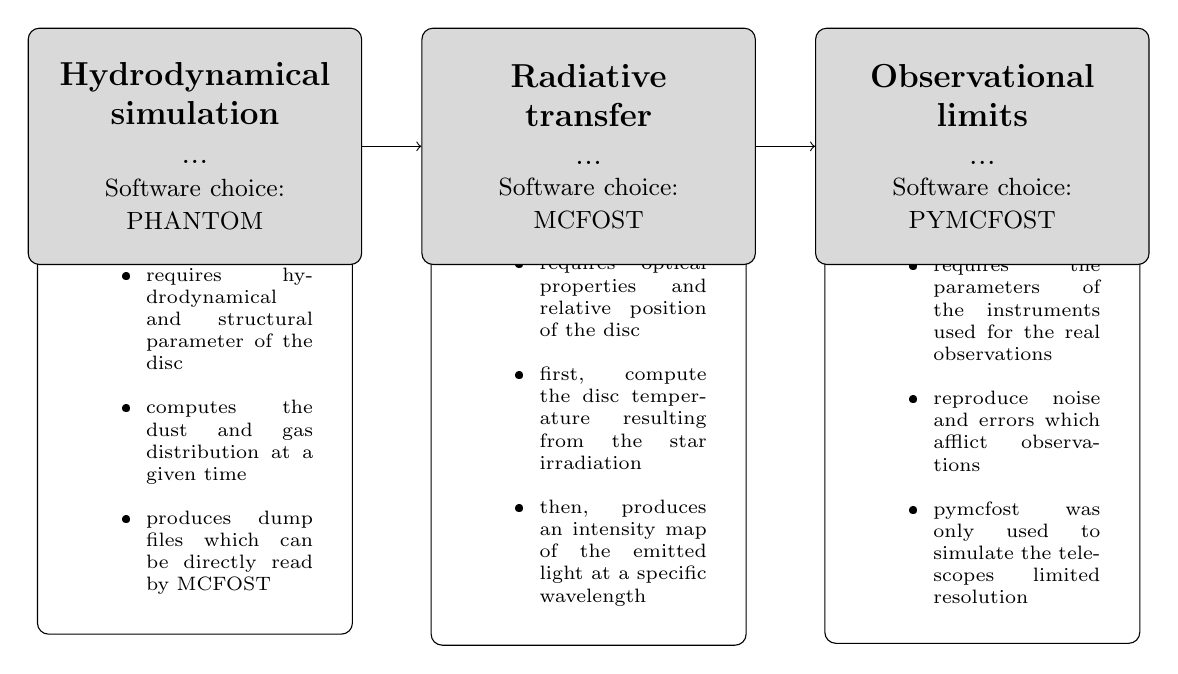
\begin{tikzpicture}
            

            %models
            \tikzstyle{block} = [rectangle, rounded corners, text width=4cm, minimum height=3cm,text centered, draw=black, fill=gray!30]
            \tikzstyle{io} = [rectangle, rounded corners,text width=4cm, minimum height=1cm,text centered, align=left, font=\scriptsize, draw=black]
            \tikzstyle{block2} = [rectangle, rounded corners, text width=3cm, minimum height=6cm,text justified, draw=black, inner sep =0.5cm]
            
            
            %main rectangles
            \node (phantom) [block] {\large \bf Hydrodynamical simulation \\ \normalfont ... \\ \small Software choice: PHANTOM};
            \node (mcfost) [block, right of=phantom, xshift=4cm]
            {\large \bf Radiative \\transfer \\ \normalfont ... \\ \small Software choice: \\ MCFOST};
            \node (pymcfost) [block, right of=mcfost, xshift=4cm] {\large \bf Observational \\limits \\ \normalfont ... \\ \small Software choice: \\ PYMCFOST};

            %arrows
            \draw [->] (phantom) -- (mcfost);
            \draw [->] (mcfost) -- (pymcfost);

            \begin{scope}[on background layer]
            \node (iph) [block2, below of=phantom, yshift=-2cm] {
                \scriptsize
                \\ \\ \\ \\
                \begin{itemize}
                    \item requires hydrodynamical and structural parameter of the disc \\
                    \item computes the dust and gas distribution at a given time \\
                    \item produces dump files which can be directly read by MCFOST
                \end{itemize}
            
            };


            \node (iph2) [block2, below of=mcfost, yshift=-2cm] {
                \scriptsize
                 \\ \\ \\ \\
                \begin{itemize}
                    \item requires optical properties and relative position of the disc \\
                    \item first, compute the disc temperature resulting from the star irradiation \\
                    \item then, produces an intensity map of the emitted light at a specific wavelength
                \end{itemize}
            
            };

            \node (iph2) [block2, below of=pymcfost, yshift=-2cm] {
                \scriptsize
                 \\ \\ \\ \\
                \begin{itemize}
                    \item requires the parameters of the instruments used for the real observations \\
                    \item reproduce noise and errors which afflict observations \\
                    \item pymcfost was only used to simulate the telescopes limited resolution
                \end{itemize}
            
            };

            \end{scope}
            \begin{comment}
            \node (iph2) [io, below of=iph, yshift=-0.5cm] 
            {
                $    \rightarrow
                \begin{cases}
                 *\_00001 \\
                 *\_00002 \\
                 ... \\
                \end{cases}$
            };
            \coordinate [right of=mcfost, yshift=1.3cm, xshift=2cm] (fn1) ;
            \coordinate  [right of=iph2, xshift=1cm] (fn2);
            
            
            %\node (imcf) [io, right of=mcfost, xshift=2.6cm, yshift=0.7cm]{ $\leftarrow$ *.para};
            %\node (uuoutmcf) [io, below of=imcf, xshift=1.5cm, yshift=0.3cm]{ $\rightleftarrows$ data\_th/Temperature.fits.gz};
            %\node (outmcf) [io, below of=uuoutmcf, xshift=-0.55cm, yshift=0.3cm]{ $\rightarrow$ data\_***/RT.fits.gz};
            
            %\coordinate [right of=pymcfost, yshift=1.3cm, xshift=2cm] (fn3) ;
            %\coordinate  [right of=outmcf, xshift=1cm] (fn4);
            %\draw[->] (outmcf) -- (fn4) |- (fn3);
            %\node (ipymc) [io, below of=fn3, xshift=1.28cm, yshift=0.1cm] {$\leftarrow$ bpa, bmaj, bmin};
            \end{comment}
            \end{tikzpicture}
    \end{center}
    \caption{Typical workflow of a numerical simulation
     aimed at reproducing a synthetic image of a protoplanetary disc}
\end{figure}

I am now going to give some insights for each of these steps. The images collected in the database for machine learning
applications that we designed, were obtained through simulations of this kind. Among the possible choices
of software available for each step, I am going to focus on the ones used to obtain the synthetic images
in this database.

\subsection{Hydrodynamical simulations}

\begin{comment}
Here I am going to give some background about phantom and the type of 
data it generates.
\end{comment}

Hydrodynamical simulations solve fluid dynamics equations to predict the evolution of the gas and dust 
modelled as fluids with the specific features discussed in section 2.2.
To run the models a starting configuration must be provided which is usually generated from given masses 
of each component and specifying, assuming axisymmetric discs, the density and sound-speed radial profiles modelled
with power laws such as:
\begin{equation}
    \Sigma(r) = \Sigma(R_{ref})\cdot\left(\frac{r}{R_{ref}}\right)^{-p}
\end{equation}
and
\begin{equation}
    c_s(r) = c_s(R_{ref})\cdot\left(\frac{r}{R_{ref}}\right)^{-q}
\end{equation}
where $R_{ref}$ is a reference radius. The density and sound-speed values at this radius, in addition to the indexes $p$ and $q$
are the input constants that characterize the initial state.
Other variables, such as the $\alpha$-viscosity, the planet and stellar masses and the orbital radius, are also provided as input parameters.

One of the available programs for this step is \lstinline{PHANTOM}, a smoothed particle hydrodynamics (SPH) code 
specifically designed for astrophysical applications and which is the one used to produce
the starting data for the synthetic images collected in the database that was developed in this thesis.
If properly compiled, \lstinline{PHANTOM} is able to run a simulation of a protoplanetary disc with a planet orbiting around the central star. 
The simulation starts from an initial condition described in the input files and produces, after each given number of completed planet orbits, a dump file
containing the spatial distribution of the gas and dust simulated particles, in addition to their velocity. 
All the information needed to restart the simulation is also stored inside these files.

\subsection{Radiative transfer}

\begin{comment}
Here I am going to discuss the software used for radiative transfer: MCFOST.
I will explain why this step is performed and the meaning of the results obtained.
\end{comment}

The next stage in the simulation workflow is the radiative transfer computation. For this
step we chose to use \lstinline{MCFOST}, a code designed for this purpose and based on Monte Carlo methods.
This program provides the possibility to run a simulation for gas and dust grains in the specific 
spatial configurations stored in a \lstinline{PHANTOM} dump file.

The aim is to obtain a synthetic observation of specific light tracers as seen from given angles and distance.
To produce the images used in this thesis we are only interested in probing the dust component through the thermally
emitted and scattered radiation at a fixed wavelength.
First of all, the radiative transfer of energy from the star to the disc elements is calculated, generating a map of the disc temperature.
At this point the thermal emission of the dust is computed and ray traced to obtain the resulting image.

The model run by \lstinline{MCFOST} depends upon optical properties, such as the optical length and the opacity, which 
are new parameters characterizing the results of the entire simulation process.

The output obtained at this stage is a 1024x1024 pixels image in the
\lstinline{FITS} (Flexible Image Transport System) format.
The header of this file stores some input parameters: 
the wavelength of the light in the image, the inclination and position angle of
the disc, its distance and the units of the data stored.

\subsection{Generation of synthetic images}

\begin{comment}
Here I am going to discuss the different methods that can be used to simulate the limitations 
of observing instruments. I will further explore some key features of pymcfost.
\end{comment}

\begin{figure}
    \begin{center}
        \scalebox{0.45}{%% Creator: Matplotlib, PGF backend
%%
%% To include the figure in your LaTeX document, write
%%   \input{<filename>.pgf}
%%
%% Make sure the required packages are loaded in your preamble
%%   \usepackage{pgf}
%%
%% Figures using additional raster images can only be included by \input if
%% they are in the same directory as the main LaTeX file. For loading figures
%% from other directories you can use the `import` package
%%   \usepackage{import}
%%
%% and then include the figures with
%%   \import{<path to file>}{<filename>.pgf}
%%
%% Matplotlib used the following preamble
%%
\begingroup%
\makeatletter%
\begin{pgfpicture}%
\pgfpathrectangle{\pgfpointorigin}{\pgfqpoint{12.900000in}{3.440280in}}%
\pgfusepath{use as bounding box, clip}%
\begin{pgfscope}%
\pgfsetbuttcap%
\pgfsetmiterjoin%
\pgfsetlinewidth{0.000000pt}%
\definecolor{currentstroke}{rgb}{1.000000,1.000000,1.000000}%
\pgfsetstrokecolor{currentstroke}%
\pgfsetstrokeopacity{0.000000}%
\pgfsetdash{}{0pt}%
\pgfpathmoveto{\pgfqpoint{0.000000in}{0.000000in}}%
\pgfpathlineto{\pgfqpoint{12.900000in}{0.000000in}}%
\pgfpathlineto{\pgfqpoint{12.900000in}{3.440280in}}%
\pgfpathlineto{\pgfqpoint{0.000000in}{3.440280in}}%
\pgfpathclose%
\pgfusepath{}%
\end{pgfscope}%
\begin{pgfscope}%
\pgfsetbuttcap%
\pgfsetmiterjoin%
\definecolor{currentfill}{rgb}{1.000000,1.000000,1.000000}%
\pgfsetfillcolor{currentfill}%
\pgfsetlinewidth{0.000000pt}%
\definecolor{currentstroke}{rgb}{0.000000,0.000000,0.000000}%
\pgfsetstrokecolor{currentstroke}%
\pgfsetstrokeopacity{0.000000}%
\pgfsetdash{}{0pt}%
\pgfpathmoveto{\pgfqpoint{0.677161in}{0.515123in}}%
\pgfpathlineto{\pgfqpoint{3.356083in}{0.515123in}}%
\pgfpathlineto{\pgfqpoint{3.356083in}{3.194045in}}%
\pgfpathlineto{\pgfqpoint{0.677161in}{3.194045in}}%
\pgfpathclose%
\pgfusepath{fill}%
\end{pgfscope}%
\begin{pgfscope}%
\pgfpathrectangle{\pgfqpoint{0.677161in}{0.515123in}}{\pgfqpoint{2.678922in}{2.678922in}}%
\pgfusepath{clip}%
\pgfsys@transformshift{0.677161in}{0.515123in}%
\pgftext[left,bottom]{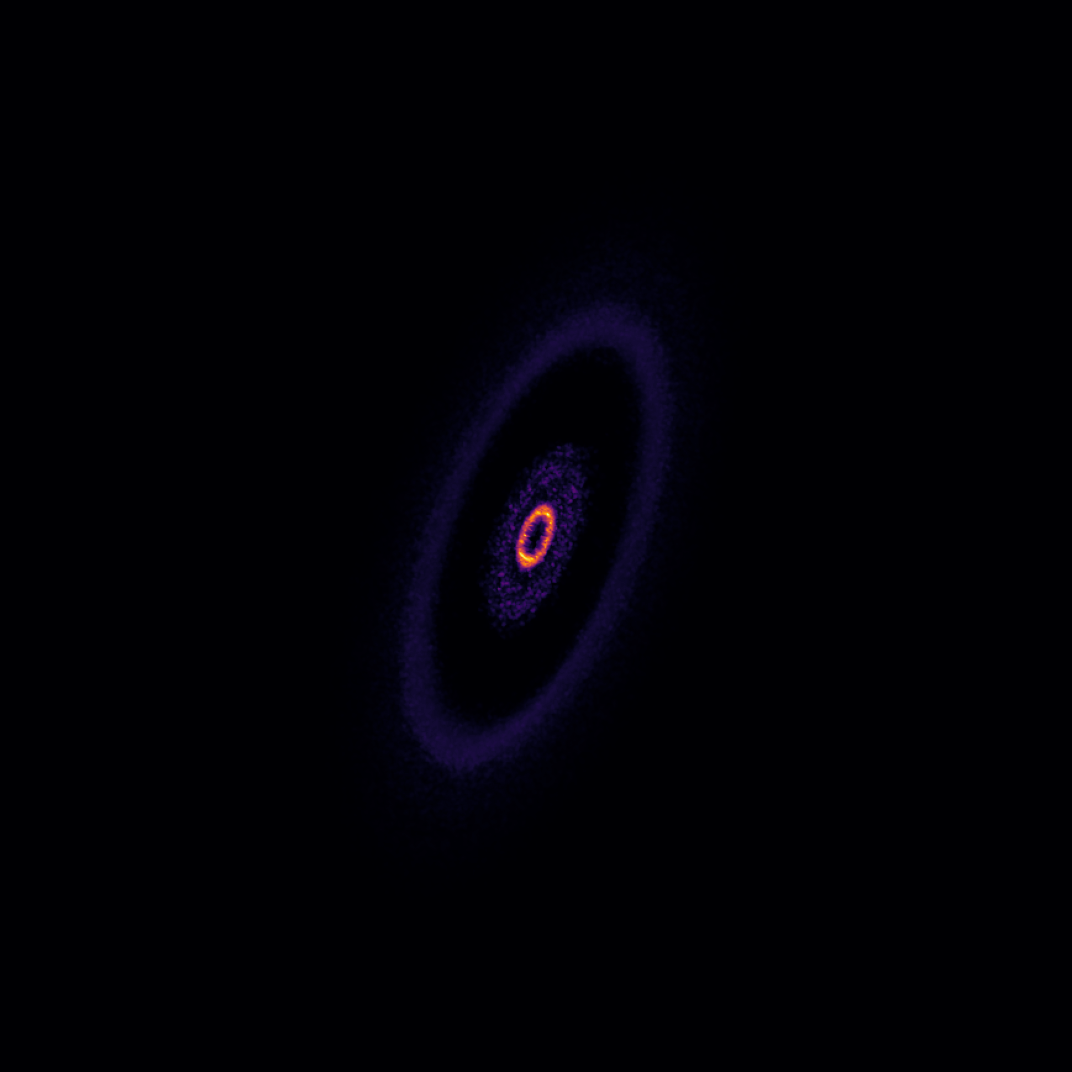
\includegraphics[interpolate=true,width=2.680000in,height=2.680000in]{images/fig3.2-img0.png}}%
\end{pgfscope}%
\begin{pgfscope}%
\pgfpathrectangle{\pgfqpoint{0.677161in}{0.515123in}}{\pgfqpoint{2.678922in}{2.678922in}}%
\pgfusepath{clip}%
\pgfsetbuttcap%
\pgfsetmiterjoin%
\definecolor{currentfill}{rgb}{0.501961,0.501961,0.501961}%
\pgfsetfillcolor{currentfill}%
\pgfsetlinewidth{1.003750pt}%
\definecolor{currentstroke}{rgb}{0.501961,0.501961,0.501961}%
\pgfsetstrokecolor{currentstroke}%
\pgfsetdash{}{0pt}%
\pgfpathmoveto{\pgfqpoint{1.012030in}{0.849996in}}%
\pgfpathcurveto{\pgfqpoint{1.012032in}{0.849996in}}{\pgfqpoint{1.012033in}{0.849994in}}{\pgfqpoint{1.012034in}{0.849992in}}%
\pgfpathcurveto{\pgfqpoint{1.012035in}{0.849990in}}{\pgfqpoint{1.012035in}{0.849988in}}{\pgfqpoint{1.012034in}{0.849986in}}%
\pgfpathcurveto{\pgfqpoint{1.012034in}{0.849983in}}{\pgfqpoint{1.012032in}{0.849982in}}{\pgfqpoint{1.012030in}{0.849981in}}%
\pgfpathcurveto{\pgfqpoint{1.012028in}{0.849980in}}{\pgfqpoint{1.012026in}{0.849980in}}{\pgfqpoint{1.012024in}{0.849981in}}%
\pgfpathcurveto{\pgfqpoint{1.012022in}{0.849982in}}{\pgfqpoint{1.012020in}{0.849983in}}{\pgfqpoint{1.012019in}{0.849985in}}%
\pgfpathcurveto{\pgfqpoint{1.012018in}{0.849987in}}{\pgfqpoint{1.012018in}{0.849989in}}{\pgfqpoint{1.012019in}{0.849992in}}%
\pgfpathcurveto{\pgfqpoint{1.012020in}{0.849994in}}{\pgfqpoint{1.012021in}{0.849995in}}{\pgfqpoint{1.012023in}{0.849996in}}%
\pgfpathcurveto{\pgfqpoint{1.012025in}{0.849997in}}{\pgfqpoint{1.012028in}{0.849997in}}{\pgfqpoint{1.012030in}{0.849996in}}%
\pgfpathclose%
\pgfusepath{stroke,fill}%
\end{pgfscope}%
\begin{pgfscope}%
\pgfsetbuttcap%
\pgfsetroundjoin%
\definecolor{currentfill}{rgb}{0.000000,0.000000,0.000000}%
\pgfsetfillcolor{currentfill}%
\pgfsetlinewidth{0.803000pt}%
\definecolor{currentstroke}{rgb}{0.000000,0.000000,0.000000}%
\pgfsetstrokecolor{currentstroke}%
\pgfsetdash{}{0pt}%
\pgfsys@defobject{currentmarker}{\pgfqpoint{0.000000in}{-0.048611in}}{\pgfqpoint{0.000000in}{0.000000in}}{%
\pgfpathmoveto{\pgfqpoint{0.000000in}{0.000000in}}%
\pgfpathlineto{\pgfqpoint{0.000000in}{-0.048611in}}%
\pgfusepath{stroke,fill}%
}%
\begin{pgfscope}%
\pgfsys@transformshift{2.853785in}{0.515123in}%
\pgfsys@useobject{currentmarker}{}%
\end{pgfscope}%
\end{pgfscope}%
\begin{pgfscope}%
\definecolor{textcolor}{rgb}{0.000000,0.000000,0.000000}%
\pgfsetstrokecolor{textcolor}%
\pgfsetfillcolor{textcolor}%
\pgftext[x=2.853785in,y=0.417901in,,top]{\color{textcolor}\rmfamily\fontsize{10.000000}{12.000000}\selectfont \(\displaystyle {\ensuremath{-}0.5}\)}%
\end{pgfscope}%
\begin{pgfscope}%
\pgfsetbuttcap%
\pgfsetroundjoin%
\definecolor{currentfill}{rgb}{0.000000,0.000000,0.000000}%
\pgfsetfillcolor{currentfill}%
\pgfsetlinewidth{0.803000pt}%
\definecolor{currentstroke}{rgb}{0.000000,0.000000,0.000000}%
\pgfsetstrokecolor{currentstroke}%
\pgfsetdash{}{0pt}%
\pgfsys@defobject{currentmarker}{\pgfqpoint{0.000000in}{-0.048611in}}{\pgfqpoint{0.000000in}{0.000000in}}{%
\pgfpathmoveto{\pgfqpoint{0.000000in}{0.000000in}}%
\pgfpathlineto{\pgfqpoint{0.000000in}{-0.048611in}}%
\pgfusepath{stroke,fill}%
}%
\begin{pgfscope}%
\pgfsys@transformshift{2.016622in}{0.515123in}%
\pgfsys@useobject{currentmarker}{}%
\end{pgfscope}%
\end{pgfscope}%
\begin{pgfscope}%
\definecolor{textcolor}{rgb}{0.000000,0.000000,0.000000}%
\pgfsetstrokecolor{textcolor}%
\pgfsetfillcolor{textcolor}%
\pgftext[x=2.016622in,y=0.417901in,,top]{\color{textcolor}\rmfamily\fontsize{10.000000}{12.000000}\selectfont \(\displaystyle {0.0}\)}%
\end{pgfscope}%
\begin{pgfscope}%
\pgfsetbuttcap%
\pgfsetroundjoin%
\definecolor{currentfill}{rgb}{0.000000,0.000000,0.000000}%
\pgfsetfillcolor{currentfill}%
\pgfsetlinewidth{0.803000pt}%
\definecolor{currentstroke}{rgb}{0.000000,0.000000,0.000000}%
\pgfsetstrokecolor{currentstroke}%
\pgfsetdash{}{0pt}%
\pgfsys@defobject{currentmarker}{\pgfqpoint{0.000000in}{-0.048611in}}{\pgfqpoint{0.000000in}{0.000000in}}{%
\pgfpathmoveto{\pgfqpoint{0.000000in}{0.000000in}}%
\pgfpathlineto{\pgfqpoint{0.000000in}{-0.048611in}}%
\pgfusepath{stroke,fill}%
}%
\begin{pgfscope}%
\pgfsys@transformshift{1.179459in}{0.515123in}%
\pgfsys@useobject{currentmarker}{}%
\end{pgfscope}%
\end{pgfscope}%
\begin{pgfscope}%
\definecolor{textcolor}{rgb}{0.000000,0.000000,0.000000}%
\pgfsetstrokecolor{textcolor}%
\pgfsetfillcolor{textcolor}%
\pgftext[x=1.179459in,y=0.417901in,,top]{\color{textcolor}\rmfamily\fontsize{10.000000}{12.000000}\selectfont \(\displaystyle {0.5}\)}%
\end{pgfscope}%
\begin{pgfscope}%
\definecolor{textcolor}{rgb}{0.000000,0.000000,0.000000}%
\pgfsetstrokecolor{textcolor}%
\pgfsetfillcolor{textcolor}%
\pgftext[x=2.016622in,y=0.238889in,,top]{\color{textcolor}\rmfamily\fontsize{10.000000}{12.000000}\selectfont \(\displaystyle \Delta RA [^\circ]\)}%
\end{pgfscope}%
\begin{pgfscope}%
\pgfsetbuttcap%
\pgfsetroundjoin%
\definecolor{currentfill}{rgb}{0.000000,0.000000,0.000000}%
\pgfsetfillcolor{currentfill}%
\pgfsetlinewidth{0.803000pt}%
\definecolor{currentstroke}{rgb}{0.000000,0.000000,0.000000}%
\pgfsetstrokecolor{currentstroke}%
\pgfsetdash{}{0pt}%
\pgfsys@defobject{currentmarker}{\pgfqpoint{-0.048611in}{0.000000in}}{\pgfqpoint{-0.000000in}{0.000000in}}{%
\pgfpathmoveto{\pgfqpoint{-0.000000in}{0.000000in}}%
\pgfpathlineto{\pgfqpoint{-0.048611in}{0.000000in}}%
\pgfusepath{stroke,fill}%
}%
\begin{pgfscope}%
\pgfsys@transformshift{0.677161in}{0.515123in}%
\pgfsys@useobject{currentmarker}{}%
\end{pgfscope}%
\end{pgfscope}%
\begin{pgfscope}%
\definecolor{textcolor}{rgb}{0.000000,0.000000,0.000000}%
\pgfsetstrokecolor{textcolor}%
\pgfsetfillcolor{textcolor}%
\pgftext[x=0.294444in, y=0.466898in, left, base]{\color{textcolor}\rmfamily\fontsize{10.000000}{12.000000}\selectfont \(\displaystyle {\ensuremath{-}0.8}\)}%
\end{pgfscope}%
\begin{pgfscope}%
\pgfsetbuttcap%
\pgfsetroundjoin%
\definecolor{currentfill}{rgb}{0.000000,0.000000,0.000000}%
\pgfsetfillcolor{currentfill}%
\pgfsetlinewidth{0.803000pt}%
\definecolor{currentstroke}{rgb}{0.000000,0.000000,0.000000}%
\pgfsetstrokecolor{currentstroke}%
\pgfsetdash{}{0pt}%
\pgfsys@defobject{currentmarker}{\pgfqpoint{-0.048611in}{0.000000in}}{\pgfqpoint{-0.000000in}{0.000000in}}{%
\pgfpathmoveto{\pgfqpoint{-0.000000in}{0.000000in}}%
\pgfpathlineto{\pgfqpoint{-0.048611in}{0.000000in}}%
\pgfusepath{stroke,fill}%
}%
\begin{pgfscope}%
\pgfsys@transformshift{0.677161in}{0.849989in}%
\pgfsys@useobject{currentmarker}{}%
\end{pgfscope}%
\end{pgfscope}%
\begin{pgfscope}%
\definecolor{textcolor}{rgb}{0.000000,0.000000,0.000000}%
\pgfsetstrokecolor{textcolor}%
\pgfsetfillcolor{textcolor}%
\pgftext[x=0.294444in, y=0.801763in, left, base]{\color{textcolor}\rmfamily\fontsize{10.000000}{12.000000}\selectfont \(\displaystyle {\ensuremath{-}0.6}\)}%
\end{pgfscope}%
\begin{pgfscope}%
\pgfsetbuttcap%
\pgfsetroundjoin%
\definecolor{currentfill}{rgb}{0.000000,0.000000,0.000000}%
\pgfsetfillcolor{currentfill}%
\pgfsetlinewidth{0.803000pt}%
\definecolor{currentstroke}{rgb}{0.000000,0.000000,0.000000}%
\pgfsetstrokecolor{currentstroke}%
\pgfsetdash{}{0pt}%
\pgfsys@defobject{currentmarker}{\pgfqpoint{-0.048611in}{0.000000in}}{\pgfqpoint{-0.000000in}{0.000000in}}{%
\pgfpathmoveto{\pgfqpoint{-0.000000in}{0.000000in}}%
\pgfpathlineto{\pgfqpoint{-0.048611in}{0.000000in}}%
\pgfusepath{stroke,fill}%
}%
\begin{pgfscope}%
\pgfsys@transformshift{0.677161in}{1.184854in}%
\pgfsys@useobject{currentmarker}{}%
\end{pgfscope}%
\end{pgfscope}%
\begin{pgfscope}%
\definecolor{textcolor}{rgb}{0.000000,0.000000,0.000000}%
\pgfsetstrokecolor{textcolor}%
\pgfsetfillcolor{textcolor}%
\pgftext[x=0.294444in, y=1.136629in, left, base]{\color{textcolor}\rmfamily\fontsize{10.000000}{12.000000}\selectfont \(\displaystyle {\ensuremath{-}0.4}\)}%
\end{pgfscope}%
\begin{pgfscope}%
\pgfsetbuttcap%
\pgfsetroundjoin%
\definecolor{currentfill}{rgb}{0.000000,0.000000,0.000000}%
\pgfsetfillcolor{currentfill}%
\pgfsetlinewidth{0.803000pt}%
\definecolor{currentstroke}{rgb}{0.000000,0.000000,0.000000}%
\pgfsetstrokecolor{currentstroke}%
\pgfsetdash{}{0pt}%
\pgfsys@defobject{currentmarker}{\pgfqpoint{-0.048611in}{0.000000in}}{\pgfqpoint{-0.000000in}{0.000000in}}{%
\pgfpathmoveto{\pgfqpoint{-0.000000in}{0.000000in}}%
\pgfpathlineto{\pgfqpoint{-0.048611in}{0.000000in}}%
\pgfusepath{stroke,fill}%
}%
\begin{pgfscope}%
\pgfsys@transformshift{0.677161in}{1.519719in}%
\pgfsys@useobject{currentmarker}{}%
\end{pgfscope}%
\end{pgfscope}%
\begin{pgfscope}%
\definecolor{textcolor}{rgb}{0.000000,0.000000,0.000000}%
\pgfsetstrokecolor{textcolor}%
\pgfsetfillcolor{textcolor}%
\pgftext[x=0.294444in, y=1.471494in, left, base]{\color{textcolor}\rmfamily\fontsize{10.000000}{12.000000}\selectfont \(\displaystyle {\ensuremath{-}0.2}\)}%
\end{pgfscope}%
\begin{pgfscope}%
\pgfsetbuttcap%
\pgfsetroundjoin%
\definecolor{currentfill}{rgb}{0.000000,0.000000,0.000000}%
\pgfsetfillcolor{currentfill}%
\pgfsetlinewidth{0.803000pt}%
\definecolor{currentstroke}{rgb}{0.000000,0.000000,0.000000}%
\pgfsetstrokecolor{currentstroke}%
\pgfsetdash{}{0pt}%
\pgfsys@defobject{currentmarker}{\pgfqpoint{-0.048611in}{0.000000in}}{\pgfqpoint{-0.000000in}{0.000000in}}{%
\pgfpathmoveto{\pgfqpoint{-0.000000in}{0.000000in}}%
\pgfpathlineto{\pgfqpoint{-0.048611in}{0.000000in}}%
\pgfusepath{stroke,fill}%
}%
\begin{pgfscope}%
\pgfsys@transformshift{0.677161in}{1.854584in}%
\pgfsys@useobject{currentmarker}{}%
\end{pgfscope}%
\end{pgfscope}%
\begin{pgfscope}%
\definecolor{textcolor}{rgb}{0.000000,0.000000,0.000000}%
\pgfsetstrokecolor{textcolor}%
\pgfsetfillcolor{textcolor}%
\pgftext[x=0.402469in, y=1.806359in, left, base]{\color{textcolor}\rmfamily\fontsize{10.000000}{12.000000}\selectfont \(\displaystyle {0.0}\)}%
\end{pgfscope}%
\begin{pgfscope}%
\pgfsetbuttcap%
\pgfsetroundjoin%
\definecolor{currentfill}{rgb}{0.000000,0.000000,0.000000}%
\pgfsetfillcolor{currentfill}%
\pgfsetlinewidth{0.803000pt}%
\definecolor{currentstroke}{rgb}{0.000000,0.000000,0.000000}%
\pgfsetstrokecolor{currentstroke}%
\pgfsetdash{}{0pt}%
\pgfsys@defobject{currentmarker}{\pgfqpoint{-0.048611in}{0.000000in}}{\pgfqpoint{-0.000000in}{0.000000in}}{%
\pgfpathmoveto{\pgfqpoint{-0.000000in}{0.000000in}}%
\pgfpathlineto{\pgfqpoint{-0.048611in}{0.000000in}}%
\pgfusepath{stroke,fill}%
}%
\begin{pgfscope}%
\pgfsys@transformshift{0.677161in}{2.189449in}%
\pgfsys@useobject{currentmarker}{}%
\end{pgfscope}%
\end{pgfscope}%
\begin{pgfscope}%
\definecolor{textcolor}{rgb}{0.000000,0.000000,0.000000}%
\pgfsetstrokecolor{textcolor}%
\pgfsetfillcolor{textcolor}%
\pgftext[x=0.402469in, y=2.141224in, left, base]{\color{textcolor}\rmfamily\fontsize{10.000000}{12.000000}\selectfont \(\displaystyle {0.2}\)}%
\end{pgfscope}%
\begin{pgfscope}%
\pgfsetbuttcap%
\pgfsetroundjoin%
\definecolor{currentfill}{rgb}{0.000000,0.000000,0.000000}%
\pgfsetfillcolor{currentfill}%
\pgfsetlinewidth{0.803000pt}%
\definecolor{currentstroke}{rgb}{0.000000,0.000000,0.000000}%
\pgfsetstrokecolor{currentstroke}%
\pgfsetdash{}{0pt}%
\pgfsys@defobject{currentmarker}{\pgfqpoint{-0.048611in}{0.000000in}}{\pgfqpoint{-0.000000in}{0.000000in}}{%
\pgfpathmoveto{\pgfqpoint{-0.000000in}{0.000000in}}%
\pgfpathlineto{\pgfqpoint{-0.048611in}{0.000000in}}%
\pgfusepath{stroke,fill}%
}%
\begin{pgfscope}%
\pgfsys@transformshift{0.677161in}{2.524315in}%
\pgfsys@useobject{currentmarker}{}%
\end{pgfscope}%
\end{pgfscope}%
\begin{pgfscope}%
\definecolor{textcolor}{rgb}{0.000000,0.000000,0.000000}%
\pgfsetstrokecolor{textcolor}%
\pgfsetfillcolor{textcolor}%
\pgftext[x=0.402469in, y=2.476089in, left, base]{\color{textcolor}\rmfamily\fontsize{10.000000}{12.000000}\selectfont \(\displaystyle {0.4}\)}%
\end{pgfscope}%
\begin{pgfscope}%
\pgfsetbuttcap%
\pgfsetroundjoin%
\definecolor{currentfill}{rgb}{0.000000,0.000000,0.000000}%
\pgfsetfillcolor{currentfill}%
\pgfsetlinewidth{0.803000pt}%
\definecolor{currentstroke}{rgb}{0.000000,0.000000,0.000000}%
\pgfsetstrokecolor{currentstroke}%
\pgfsetdash{}{0pt}%
\pgfsys@defobject{currentmarker}{\pgfqpoint{-0.048611in}{0.000000in}}{\pgfqpoint{-0.000000in}{0.000000in}}{%
\pgfpathmoveto{\pgfqpoint{-0.000000in}{0.000000in}}%
\pgfpathlineto{\pgfqpoint{-0.048611in}{0.000000in}}%
\pgfusepath{stroke,fill}%
}%
\begin{pgfscope}%
\pgfsys@transformshift{0.677161in}{2.859180in}%
\pgfsys@useobject{currentmarker}{}%
\end{pgfscope}%
\end{pgfscope}%
\begin{pgfscope}%
\definecolor{textcolor}{rgb}{0.000000,0.000000,0.000000}%
\pgfsetstrokecolor{textcolor}%
\pgfsetfillcolor{textcolor}%
\pgftext[x=0.402469in, y=2.810955in, left, base]{\color{textcolor}\rmfamily\fontsize{10.000000}{12.000000}\selectfont \(\displaystyle {0.6}\)}%
\end{pgfscope}%
\begin{pgfscope}%
\pgfsetbuttcap%
\pgfsetroundjoin%
\definecolor{currentfill}{rgb}{0.000000,0.000000,0.000000}%
\pgfsetfillcolor{currentfill}%
\pgfsetlinewidth{0.803000pt}%
\definecolor{currentstroke}{rgb}{0.000000,0.000000,0.000000}%
\pgfsetstrokecolor{currentstroke}%
\pgfsetdash{}{0pt}%
\pgfsys@defobject{currentmarker}{\pgfqpoint{-0.048611in}{0.000000in}}{\pgfqpoint{-0.000000in}{0.000000in}}{%
\pgfpathmoveto{\pgfqpoint{-0.000000in}{0.000000in}}%
\pgfpathlineto{\pgfqpoint{-0.048611in}{0.000000in}}%
\pgfusepath{stroke,fill}%
}%
\begin{pgfscope}%
\pgfsys@transformshift{0.677161in}{3.194045in}%
\pgfsys@useobject{currentmarker}{}%
\end{pgfscope}%
\end{pgfscope}%
\begin{pgfscope}%
\definecolor{textcolor}{rgb}{0.000000,0.000000,0.000000}%
\pgfsetstrokecolor{textcolor}%
\pgfsetfillcolor{textcolor}%
\pgftext[x=0.402469in, y=3.145820in, left, base]{\color{textcolor}\rmfamily\fontsize{10.000000}{12.000000}\selectfont \(\displaystyle {0.8}\)}%
\end{pgfscope}%
\begin{pgfscope}%
\definecolor{textcolor}{rgb}{0.000000,0.000000,0.000000}%
\pgfsetstrokecolor{textcolor}%
\pgfsetfillcolor{textcolor}%
\pgftext[x=0.238889in,y=1.854584in,,bottom,rotate=90.000000]{\color{textcolor}\rmfamily\fontsize{10.000000}{12.000000}\selectfont \(\displaystyle \Delta Dec [^\circ]\)}%
\end{pgfscope}%
\begin{pgfscope}%
\pgfsetrectcap%
\pgfsetmiterjoin%
\pgfsetlinewidth{0.803000pt}%
\definecolor{currentstroke}{rgb}{0.000000,0.000000,0.000000}%
\pgfsetstrokecolor{currentstroke}%
\pgfsetdash{}{0pt}%
\pgfpathmoveto{\pgfqpoint{0.677161in}{0.515123in}}%
\pgfpathlineto{\pgfqpoint{0.677161in}{3.194045in}}%
\pgfusepath{stroke}%
\end{pgfscope}%
\begin{pgfscope}%
\pgfsetrectcap%
\pgfsetmiterjoin%
\pgfsetlinewidth{0.803000pt}%
\definecolor{currentstroke}{rgb}{0.000000,0.000000,0.000000}%
\pgfsetstrokecolor{currentstroke}%
\pgfsetdash{}{0pt}%
\pgfpathmoveto{\pgfqpoint{3.356083in}{0.515123in}}%
\pgfpathlineto{\pgfqpoint{3.356083in}{3.194045in}}%
\pgfusepath{stroke}%
\end{pgfscope}%
\begin{pgfscope}%
\pgfsetrectcap%
\pgfsetmiterjoin%
\pgfsetlinewidth{0.803000pt}%
\definecolor{currentstroke}{rgb}{0.000000,0.000000,0.000000}%
\pgfsetstrokecolor{currentstroke}%
\pgfsetdash{}{0pt}%
\pgfpathmoveto{\pgfqpoint{0.677161in}{0.515123in}}%
\pgfpathlineto{\pgfqpoint{3.356083in}{0.515123in}}%
\pgfusepath{stroke}%
\end{pgfscope}%
\begin{pgfscope}%
\pgfsetrectcap%
\pgfsetmiterjoin%
\pgfsetlinewidth{0.803000pt}%
\definecolor{currentstroke}{rgb}{0.000000,0.000000,0.000000}%
\pgfsetstrokecolor{currentstroke}%
\pgfsetdash{}{0pt}%
\pgfpathmoveto{\pgfqpoint{0.677161in}{3.194045in}}%
\pgfpathlineto{\pgfqpoint{3.356083in}{3.194045in}}%
\pgfusepath{stroke}%
\end{pgfscope}%
\begin{pgfscope}%
\pgfsetbuttcap%
\pgfsetmiterjoin%
\definecolor{currentfill}{rgb}{1.000000,1.000000,1.000000}%
\pgfsetfillcolor{currentfill}%
\pgfsetlinewidth{0.000000pt}%
\definecolor{currentstroke}{rgb}{0.000000,0.000000,0.000000}%
\pgfsetstrokecolor{currentstroke}%
\pgfsetstrokeopacity{0.000000}%
\pgfsetdash{}{0pt}%
\pgfpathmoveto{\pgfqpoint{4.960495in}{0.515123in}}%
\pgfpathlineto{\pgfqpoint{7.639417in}{0.515123in}}%
\pgfpathlineto{\pgfqpoint{7.639417in}{3.194045in}}%
\pgfpathlineto{\pgfqpoint{4.960495in}{3.194045in}}%
\pgfpathclose%
\pgfusepath{fill}%
\end{pgfscope}%
\begin{pgfscope}%
\pgfpathrectangle{\pgfqpoint{4.960495in}{0.515123in}}{\pgfqpoint{2.678922in}{2.678922in}}%
\pgfusepath{clip}%
\pgfsys@transformshift{4.960495in}{0.515123in}%
\pgftext[left,bottom]{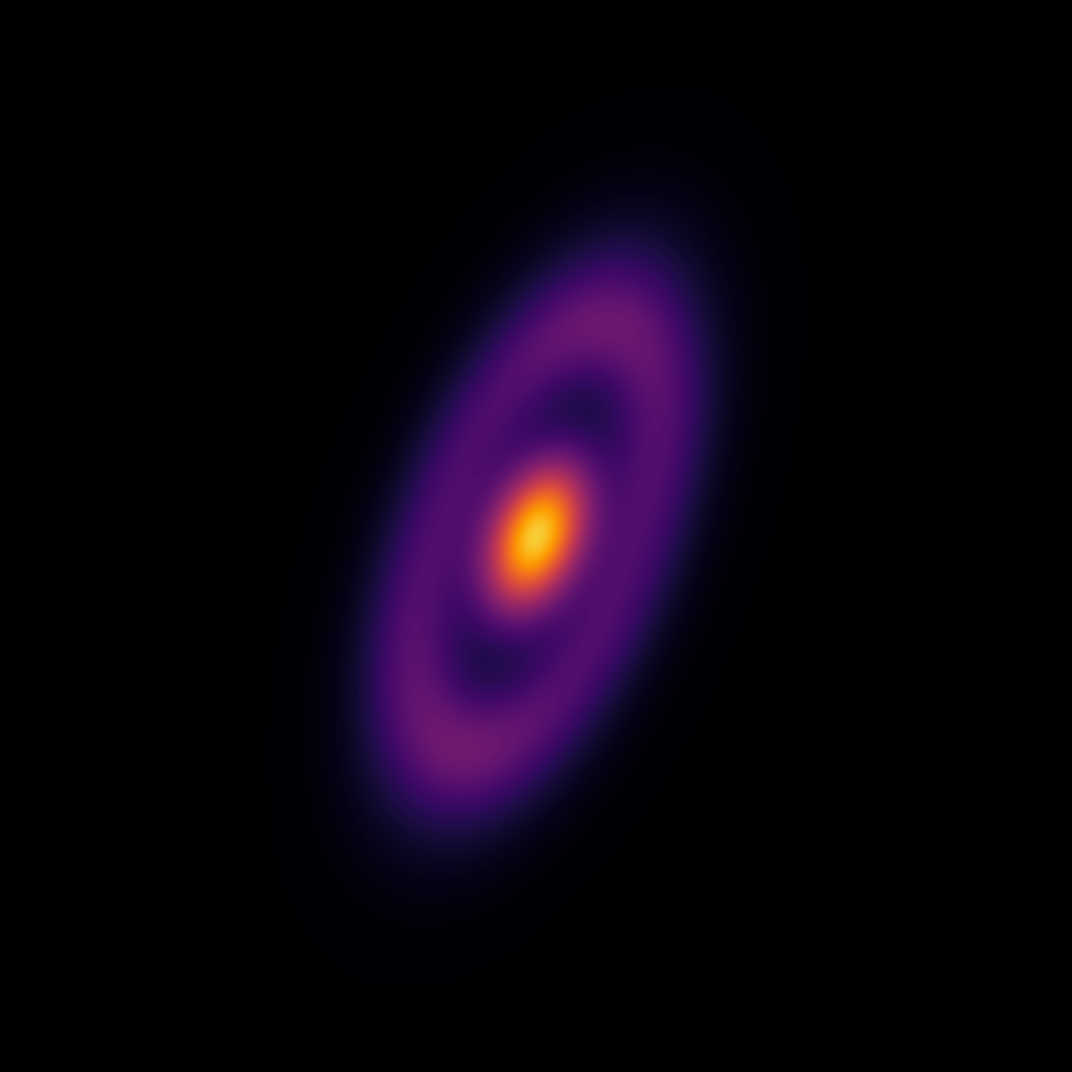
\includegraphics[interpolate=true,width=2.680000in,height=2.680000in]{images/fig3.2-img1.png}}%
\end{pgfscope}%
\begin{pgfscope}%
\pgfpathrectangle{\pgfqpoint{4.960495in}{0.515123in}}{\pgfqpoint{2.678922in}{2.678922in}}%
\pgfusepath{clip}%
\pgfsetbuttcap%
\pgfsetmiterjoin%
\definecolor{currentfill}{rgb}{0.501961,0.501961,0.501961}%
\pgfsetfillcolor{currentfill}%
\pgfsetlinewidth{1.003750pt}%
\definecolor{currentstroke}{rgb}{0.501961,0.501961,0.501961}%
\pgfsetstrokecolor{currentstroke}%
\pgfsetdash{}{0pt}%
\pgfpathmoveto{\pgfqpoint{5.337362in}{0.959407in}}%
\pgfpathcurveto{\pgfqpoint{5.358089in}{0.951450in}}{\pgfqpoint{5.373544in}{0.932290in}}{\pgfqpoint{5.380324in}{0.906145in}}%
\pgfpathcurveto{\pgfqpoint{5.387104in}{0.880000in}}{\pgfqpoint{5.384655in}{0.849005in}}{\pgfqpoint{5.373516in}{0.819987in}}%
\pgfpathcurveto{\pgfqpoint{5.362377in}{0.790969in}}{\pgfqpoint{5.343458in}{0.766297in}}{\pgfqpoint{5.320925in}{0.751404in}}%
\pgfpathcurveto{\pgfqpoint{5.298392in}{0.736511in}}{\pgfqpoint{5.274085in}{0.732614in}}{\pgfqpoint{5.253358in}{0.740570in}}%
\pgfpathcurveto{\pgfqpoint{5.232631in}{0.748527in}}{\pgfqpoint{5.217176in}{0.767687in}}{\pgfqpoint{5.210396in}{0.793832in}}%
\pgfpathcurveto{\pgfqpoint{5.203616in}{0.819977in}}{\pgfqpoint{5.206065in}{0.850972in}}{\pgfqpoint{5.217204in}{0.879990in}}%
\pgfpathcurveto{\pgfqpoint{5.228343in}{0.909008in}}{\pgfqpoint{5.247262in}{0.933680in}}{\pgfqpoint{5.269795in}{0.948573in}}%
\pgfpathcurveto{\pgfqpoint{5.292328in}{0.963466in}}{\pgfqpoint{5.316634in}{0.967363in}}{\pgfqpoint{5.337362in}{0.959407in}}%
\pgfpathclose%
\pgfusepath{stroke,fill}%
\end{pgfscope}%
\begin{pgfscope}%
\pgfsetbuttcap%
\pgfsetroundjoin%
\definecolor{currentfill}{rgb}{0.000000,0.000000,0.000000}%
\pgfsetfillcolor{currentfill}%
\pgfsetlinewidth{0.803000pt}%
\definecolor{currentstroke}{rgb}{0.000000,0.000000,0.000000}%
\pgfsetstrokecolor{currentstroke}%
\pgfsetdash{}{0pt}%
\pgfsys@defobject{currentmarker}{\pgfqpoint{0.000000in}{-0.048611in}}{\pgfqpoint{0.000000in}{0.000000in}}{%
\pgfpathmoveto{\pgfqpoint{0.000000in}{0.000000in}}%
\pgfpathlineto{\pgfqpoint{0.000000in}{-0.048611in}}%
\pgfusepath{stroke,fill}%
}%
\begin{pgfscope}%
\pgfsys@transformshift{7.137119in}{0.515123in}%
\pgfsys@useobject{currentmarker}{}%
\end{pgfscope}%
\end{pgfscope}%
\begin{pgfscope}%
\definecolor{textcolor}{rgb}{0.000000,0.000000,0.000000}%
\pgfsetstrokecolor{textcolor}%
\pgfsetfillcolor{textcolor}%
\pgftext[x=7.137119in,y=0.417901in,,top]{\color{textcolor}\rmfamily\fontsize{10.000000}{12.000000}\selectfont \(\displaystyle {\ensuremath{-}0.5}\)}%
\end{pgfscope}%
\begin{pgfscope}%
\pgfsetbuttcap%
\pgfsetroundjoin%
\definecolor{currentfill}{rgb}{0.000000,0.000000,0.000000}%
\pgfsetfillcolor{currentfill}%
\pgfsetlinewidth{0.803000pt}%
\definecolor{currentstroke}{rgb}{0.000000,0.000000,0.000000}%
\pgfsetstrokecolor{currentstroke}%
\pgfsetdash{}{0pt}%
\pgfsys@defobject{currentmarker}{\pgfqpoint{0.000000in}{-0.048611in}}{\pgfqpoint{0.000000in}{0.000000in}}{%
\pgfpathmoveto{\pgfqpoint{0.000000in}{0.000000in}}%
\pgfpathlineto{\pgfqpoint{0.000000in}{-0.048611in}}%
\pgfusepath{stroke,fill}%
}%
\begin{pgfscope}%
\pgfsys@transformshift{6.299956in}{0.515123in}%
\pgfsys@useobject{currentmarker}{}%
\end{pgfscope}%
\end{pgfscope}%
\begin{pgfscope}%
\definecolor{textcolor}{rgb}{0.000000,0.000000,0.000000}%
\pgfsetstrokecolor{textcolor}%
\pgfsetfillcolor{textcolor}%
\pgftext[x=6.299956in,y=0.417901in,,top]{\color{textcolor}\rmfamily\fontsize{10.000000}{12.000000}\selectfont \(\displaystyle {0.0}\)}%
\end{pgfscope}%
\begin{pgfscope}%
\pgfsetbuttcap%
\pgfsetroundjoin%
\definecolor{currentfill}{rgb}{0.000000,0.000000,0.000000}%
\pgfsetfillcolor{currentfill}%
\pgfsetlinewidth{0.803000pt}%
\definecolor{currentstroke}{rgb}{0.000000,0.000000,0.000000}%
\pgfsetstrokecolor{currentstroke}%
\pgfsetdash{}{0pt}%
\pgfsys@defobject{currentmarker}{\pgfqpoint{0.000000in}{-0.048611in}}{\pgfqpoint{0.000000in}{0.000000in}}{%
\pgfpathmoveto{\pgfqpoint{0.000000in}{0.000000in}}%
\pgfpathlineto{\pgfqpoint{0.000000in}{-0.048611in}}%
\pgfusepath{stroke,fill}%
}%
\begin{pgfscope}%
\pgfsys@transformshift{5.462793in}{0.515123in}%
\pgfsys@useobject{currentmarker}{}%
\end{pgfscope}%
\end{pgfscope}%
\begin{pgfscope}%
\definecolor{textcolor}{rgb}{0.000000,0.000000,0.000000}%
\pgfsetstrokecolor{textcolor}%
\pgfsetfillcolor{textcolor}%
\pgftext[x=5.462793in,y=0.417901in,,top]{\color{textcolor}\rmfamily\fontsize{10.000000}{12.000000}\selectfont \(\displaystyle {0.5}\)}%
\end{pgfscope}%
\begin{pgfscope}%
\definecolor{textcolor}{rgb}{0.000000,0.000000,0.000000}%
\pgfsetstrokecolor{textcolor}%
\pgfsetfillcolor{textcolor}%
\pgftext[x=6.299956in,y=0.238889in,,top]{\color{textcolor}\rmfamily\fontsize{10.000000}{12.000000}\selectfont \(\displaystyle \Delta RA [^\circ]\)}%
\end{pgfscope}%
\begin{pgfscope}%
\pgfsetbuttcap%
\pgfsetroundjoin%
\definecolor{currentfill}{rgb}{0.000000,0.000000,0.000000}%
\pgfsetfillcolor{currentfill}%
\pgfsetlinewidth{0.803000pt}%
\definecolor{currentstroke}{rgb}{0.000000,0.000000,0.000000}%
\pgfsetstrokecolor{currentstroke}%
\pgfsetdash{}{0pt}%
\pgfsys@defobject{currentmarker}{\pgfqpoint{-0.048611in}{0.000000in}}{\pgfqpoint{-0.000000in}{0.000000in}}{%
\pgfpathmoveto{\pgfqpoint{-0.000000in}{0.000000in}}%
\pgfpathlineto{\pgfqpoint{-0.048611in}{0.000000in}}%
\pgfusepath{stroke,fill}%
}%
\begin{pgfscope}%
\pgfsys@transformshift{4.960495in}{0.515123in}%
\pgfsys@useobject{currentmarker}{}%
\end{pgfscope}%
\end{pgfscope}%
\begin{pgfscope}%
\definecolor{textcolor}{rgb}{0.000000,0.000000,0.000000}%
\pgfsetstrokecolor{textcolor}%
\pgfsetfillcolor{textcolor}%
\pgftext[x=4.577778in, y=0.466898in, left, base]{\color{textcolor}\rmfamily\fontsize{10.000000}{12.000000}\selectfont \(\displaystyle {\ensuremath{-}0.8}\)}%
\end{pgfscope}%
\begin{pgfscope}%
\pgfsetbuttcap%
\pgfsetroundjoin%
\definecolor{currentfill}{rgb}{0.000000,0.000000,0.000000}%
\pgfsetfillcolor{currentfill}%
\pgfsetlinewidth{0.803000pt}%
\definecolor{currentstroke}{rgb}{0.000000,0.000000,0.000000}%
\pgfsetstrokecolor{currentstroke}%
\pgfsetdash{}{0pt}%
\pgfsys@defobject{currentmarker}{\pgfqpoint{-0.048611in}{0.000000in}}{\pgfqpoint{-0.000000in}{0.000000in}}{%
\pgfpathmoveto{\pgfqpoint{-0.000000in}{0.000000in}}%
\pgfpathlineto{\pgfqpoint{-0.048611in}{0.000000in}}%
\pgfusepath{stroke,fill}%
}%
\begin{pgfscope}%
\pgfsys@transformshift{4.960495in}{0.849989in}%
\pgfsys@useobject{currentmarker}{}%
\end{pgfscope}%
\end{pgfscope}%
\begin{pgfscope}%
\definecolor{textcolor}{rgb}{0.000000,0.000000,0.000000}%
\pgfsetstrokecolor{textcolor}%
\pgfsetfillcolor{textcolor}%
\pgftext[x=4.577778in, y=0.801763in, left, base]{\color{textcolor}\rmfamily\fontsize{10.000000}{12.000000}\selectfont \(\displaystyle {\ensuremath{-}0.6}\)}%
\end{pgfscope}%
\begin{pgfscope}%
\pgfsetbuttcap%
\pgfsetroundjoin%
\definecolor{currentfill}{rgb}{0.000000,0.000000,0.000000}%
\pgfsetfillcolor{currentfill}%
\pgfsetlinewidth{0.803000pt}%
\definecolor{currentstroke}{rgb}{0.000000,0.000000,0.000000}%
\pgfsetstrokecolor{currentstroke}%
\pgfsetdash{}{0pt}%
\pgfsys@defobject{currentmarker}{\pgfqpoint{-0.048611in}{0.000000in}}{\pgfqpoint{-0.000000in}{0.000000in}}{%
\pgfpathmoveto{\pgfqpoint{-0.000000in}{0.000000in}}%
\pgfpathlineto{\pgfqpoint{-0.048611in}{0.000000in}}%
\pgfusepath{stroke,fill}%
}%
\begin{pgfscope}%
\pgfsys@transformshift{4.960495in}{1.184854in}%
\pgfsys@useobject{currentmarker}{}%
\end{pgfscope}%
\end{pgfscope}%
\begin{pgfscope}%
\definecolor{textcolor}{rgb}{0.000000,0.000000,0.000000}%
\pgfsetstrokecolor{textcolor}%
\pgfsetfillcolor{textcolor}%
\pgftext[x=4.577778in, y=1.136629in, left, base]{\color{textcolor}\rmfamily\fontsize{10.000000}{12.000000}\selectfont \(\displaystyle {\ensuremath{-}0.4}\)}%
\end{pgfscope}%
\begin{pgfscope}%
\pgfsetbuttcap%
\pgfsetroundjoin%
\definecolor{currentfill}{rgb}{0.000000,0.000000,0.000000}%
\pgfsetfillcolor{currentfill}%
\pgfsetlinewidth{0.803000pt}%
\definecolor{currentstroke}{rgb}{0.000000,0.000000,0.000000}%
\pgfsetstrokecolor{currentstroke}%
\pgfsetdash{}{0pt}%
\pgfsys@defobject{currentmarker}{\pgfqpoint{-0.048611in}{0.000000in}}{\pgfqpoint{-0.000000in}{0.000000in}}{%
\pgfpathmoveto{\pgfqpoint{-0.000000in}{0.000000in}}%
\pgfpathlineto{\pgfqpoint{-0.048611in}{0.000000in}}%
\pgfusepath{stroke,fill}%
}%
\begin{pgfscope}%
\pgfsys@transformshift{4.960495in}{1.519719in}%
\pgfsys@useobject{currentmarker}{}%
\end{pgfscope}%
\end{pgfscope}%
\begin{pgfscope}%
\definecolor{textcolor}{rgb}{0.000000,0.000000,0.000000}%
\pgfsetstrokecolor{textcolor}%
\pgfsetfillcolor{textcolor}%
\pgftext[x=4.577778in, y=1.471494in, left, base]{\color{textcolor}\rmfamily\fontsize{10.000000}{12.000000}\selectfont \(\displaystyle {\ensuremath{-}0.2}\)}%
\end{pgfscope}%
\begin{pgfscope}%
\pgfsetbuttcap%
\pgfsetroundjoin%
\definecolor{currentfill}{rgb}{0.000000,0.000000,0.000000}%
\pgfsetfillcolor{currentfill}%
\pgfsetlinewidth{0.803000pt}%
\definecolor{currentstroke}{rgb}{0.000000,0.000000,0.000000}%
\pgfsetstrokecolor{currentstroke}%
\pgfsetdash{}{0pt}%
\pgfsys@defobject{currentmarker}{\pgfqpoint{-0.048611in}{0.000000in}}{\pgfqpoint{-0.000000in}{0.000000in}}{%
\pgfpathmoveto{\pgfqpoint{-0.000000in}{0.000000in}}%
\pgfpathlineto{\pgfqpoint{-0.048611in}{0.000000in}}%
\pgfusepath{stroke,fill}%
}%
\begin{pgfscope}%
\pgfsys@transformshift{4.960495in}{1.854584in}%
\pgfsys@useobject{currentmarker}{}%
\end{pgfscope}%
\end{pgfscope}%
\begin{pgfscope}%
\definecolor{textcolor}{rgb}{0.000000,0.000000,0.000000}%
\pgfsetstrokecolor{textcolor}%
\pgfsetfillcolor{textcolor}%
\pgftext[x=4.685803in, y=1.806359in, left, base]{\color{textcolor}\rmfamily\fontsize{10.000000}{12.000000}\selectfont \(\displaystyle {0.0}\)}%
\end{pgfscope}%
\begin{pgfscope}%
\pgfsetbuttcap%
\pgfsetroundjoin%
\definecolor{currentfill}{rgb}{0.000000,0.000000,0.000000}%
\pgfsetfillcolor{currentfill}%
\pgfsetlinewidth{0.803000pt}%
\definecolor{currentstroke}{rgb}{0.000000,0.000000,0.000000}%
\pgfsetstrokecolor{currentstroke}%
\pgfsetdash{}{0pt}%
\pgfsys@defobject{currentmarker}{\pgfqpoint{-0.048611in}{0.000000in}}{\pgfqpoint{-0.000000in}{0.000000in}}{%
\pgfpathmoveto{\pgfqpoint{-0.000000in}{0.000000in}}%
\pgfpathlineto{\pgfqpoint{-0.048611in}{0.000000in}}%
\pgfusepath{stroke,fill}%
}%
\begin{pgfscope}%
\pgfsys@transformshift{4.960495in}{2.189449in}%
\pgfsys@useobject{currentmarker}{}%
\end{pgfscope}%
\end{pgfscope}%
\begin{pgfscope}%
\definecolor{textcolor}{rgb}{0.000000,0.000000,0.000000}%
\pgfsetstrokecolor{textcolor}%
\pgfsetfillcolor{textcolor}%
\pgftext[x=4.685803in, y=2.141224in, left, base]{\color{textcolor}\rmfamily\fontsize{10.000000}{12.000000}\selectfont \(\displaystyle {0.2}\)}%
\end{pgfscope}%
\begin{pgfscope}%
\pgfsetbuttcap%
\pgfsetroundjoin%
\definecolor{currentfill}{rgb}{0.000000,0.000000,0.000000}%
\pgfsetfillcolor{currentfill}%
\pgfsetlinewidth{0.803000pt}%
\definecolor{currentstroke}{rgb}{0.000000,0.000000,0.000000}%
\pgfsetstrokecolor{currentstroke}%
\pgfsetdash{}{0pt}%
\pgfsys@defobject{currentmarker}{\pgfqpoint{-0.048611in}{0.000000in}}{\pgfqpoint{-0.000000in}{0.000000in}}{%
\pgfpathmoveto{\pgfqpoint{-0.000000in}{0.000000in}}%
\pgfpathlineto{\pgfqpoint{-0.048611in}{0.000000in}}%
\pgfusepath{stroke,fill}%
}%
\begin{pgfscope}%
\pgfsys@transformshift{4.960495in}{2.524315in}%
\pgfsys@useobject{currentmarker}{}%
\end{pgfscope}%
\end{pgfscope}%
\begin{pgfscope}%
\definecolor{textcolor}{rgb}{0.000000,0.000000,0.000000}%
\pgfsetstrokecolor{textcolor}%
\pgfsetfillcolor{textcolor}%
\pgftext[x=4.685803in, y=2.476089in, left, base]{\color{textcolor}\rmfamily\fontsize{10.000000}{12.000000}\selectfont \(\displaystyle {0.4}\)}%
\end{pgfscope}%
\begin{pgfscope}%
\pgfsetbuttcap%
\pgfsetroundjoin%
\definecolor{currentfill}{rgb}{0.000000,0.000000,0.000000}%
\pgfsetfillcolor{currentfill}%
\pgfsetlinewidth{0.803000pt}%
\definecolor{currentstroke}{rgb}{0.000000,0.000000,0.000000}%
\pgfsetstrokecolor{currentstroke}%
\pgfsetdash{}{0pt}%
\pgfsys@defobject{currentmarker}{\pgfqpoint{-0.048611in}{0.000000in}}{\pgfqpoint{-0.000000in}{0.000000in}}{%
\pgfpathmoveto{\pgfqpoint{-0.000000in}{0.000000in}}%
\pgfpathlineto{\pgfqpoint{-0.048611in}{0.000000in}}%
\pgfusepath{stroke,fill}%
}%
\begin{pgfscope}%
\pgfsys@transformshift{4.960495in}{2.859180in}%
\pgfsys@useobject{currentmarker}{}%
\end{pgfscope}%
\end{pgfscope}%
\begin{pgfscope}%
\definecolor{textcolor}{rgb}{0.000000,0.000000,0.000000}%
\pgfsetstrokecolor{textcolor}%
\pgfsetfillcolor{textcolor}%
\pgftext[x=4.685803in, y=2.810955in, left, base]{\color{textcolor}\rmfamily\fontsize{10.000000}{12.000000}\selectfont \(\displaystyle {0.6}\)}%
\end{pgfscope}%
\begin{pgfscope}%
\pgfsetbuttcap%
\pgfsetroundjoin%
\definecolor{currentfill}{rgb}{0.000000,0.000000,0.000000}%
\pgfsetfillcolor{currentfill}%
\pgfsetlinewidth{0.803000pt}%
\definecolor{currentstroke}{rgb}{0.000000,0.000000,0.000000}%
\pgfsetstrokecolor{currentstroke}%
\pgfsetdash{}{0pt}%
\pgfsys@defobject{currentmarker}{\pgfqpoint{-0.048611in}{0.000000in}}{\pgfqpoint{-0.000000in}{0.000000in}}{%
\pgfpathmoveto{\pgfqpoint{-0.000000in}{0.000000in}}%
\pgfpathlineto{\pgfqpoint{-0.048611in}{0.000000in}}%
\pgfusepath{stroke,fill}%
}%
\begin{pgfscope}%
\pgfsys@transformshift{4.960495in}{3.194045in}%
\pgfsys@useobject{currentmarker}{}%
\end{pgfscope}%
\end{pgfscope}%
\begin{pgfscope}%
\definecolor{textcolor}{rgb}{0.000000,0.000000,0.000000}%
\pgfsetstrokecolor{textcolor}%
\pgfsetfillcolor{textcolor}%
\pgftext[x=4.685803in, y=3.145820in, left, base]{\color{textcolor}\rmfamily\fontsize{10.000000}{12.000000}\selectfont \(\displaystyle {0.8}\)}%
\end{pgfscope}%
\begin{pgfscope}%
\definecolor{textcolor}{rgb}{0.000000,0.000000,0.000000}%
\pgfsetstrokecolor{textcolor}%
\pgfsetfillcolor{textcolor}%
\pgftext[x=4.522222in,y=1.854584in,,bottom,rotate=90.000000]{\color{textcolor}\rmfamily\fontsize{10.000000}{12.000000}\selectfont \(\displaystyle \Delta Dec [^\circ]\)}%
\end{pgfscope}%
\begin{pgfscope}%
\pgfsetrectcap%
\pgfsetmiterjoin%
\pgfsetlinewidth{0.803000pt}%
\definecolor{currentstroke}{rgb}{0.000000,0.000000,0.000000}%
\pgfsetstrokecolor{currentstroke}%
\pgfsetdash{}{0pt}%
\pgfpathmoveto{\pgfqpoint{4.960495in}{0.515123in}}%
\pgfpathlineto{\pgfqpoint{4.960495in}{3.194045in}}%
\pgfusepath{stroke}%
\end{pgfscope}%
\begin{pgfscope}%
\pgfsetrectcap%
\pgfsetmiterjoin%
\pgfsetlinewidth{0.803000pt}%
\definecolor{currentstroke}{rgb}{0.000000,0.000000,0.000000}%
\pgfsetstrokecolor{currentstroke}%
\pgfsetdash{}{0pt}%
\pgfpathmoveto{\pgfqpoint{7.639417in}{0.515123in}}%
\pgfpathlineto{\pgfqpoint{7.639417in}{3.194045in}}%
\pgfusepath{stroke}%
\end{pgfscope}%
\begin{pgfscope}%
\pgfsetrectcap%
\pgfsetmiterjoin%
\pgfsetlinewidth{0.803000pt}%
\definecolor{currentstroke}{rgb}{0.000000,0.000000,0.000000}%
\pgfsetstrokecolor{currentstroke}%
\pgfsetdash{}{0pt}%
\pgfpathmoveto{\pgfqpoint{4.960495in}{0.515123in}}%
\pgfpathlineto{\pgfqpoint{7.639417in}{0.515123in}}%
\pgfusepath{stroke}%
\end{pgfscope}%
\begin{pgfscope}%
\pgfsetrectcap%
\pgfsetmiterjoin%
\pgfsetlinewidth{0.803000pt}%
\definecolor{currentstroke}{rgb}{0.000000,0.000000,0.000000}%
\pgfsetstrokecolor{currentstroke}%
\pgfsetdash{}{0pt}%
\pgfpathmoveto{\pgfqpoint{4.960495in}{3.194045in}}%
\pgfpathlineto{\pgfqpoint{7.639417in}{3.194045in}}%
\pgfusepath{stroke}%
\end{pgfscope}%
\begin{pgfscope}%
\pgfsetbuttcap%
\pgfsetmiterjoin%
\definecolor{currentfill}{rgb}{1.000000,1.000000,1.000000}%
\pgfsetfillcolor{currentfill}%
\pgfsetlinewidth{0.000000pt}%
\definecolor{currentstroke}{rgb}{0.000000,0.000000,0.000000}%
\pgfsetstrokecolor{currentstroke}%
\pgfsetstrokeopacity{0.000000}%
\pgfsetdash{}{0pt}%
\pgfpathmoveto{\pgfqpoint{9.243828in}{0.515123in}}%
\pgfpathlineto{\pgfqpoint{11.922750in}{0.515123in}}%
\pgfpathlineto{\pgfqpoint{11.922750in}{3.194045in}}%
\pgfpathlineto{\pgfqpoint{9.243828in}{3.194045in}}%
\pgfpathclose%
\pgfusepath{fill}%
\end{pgfscope}%
\begin{pgfscope}%
\pgfpathrectangle{\pgfqpoint{9.243828in}{0.515123in}}{\pgfqpoint{2.678922in}{2.678922in}}%
\pgfusepath{clip}%
\pgfsys@transformshift{9.243828in}{0.515123in}%
\pgftext[left,bottom]{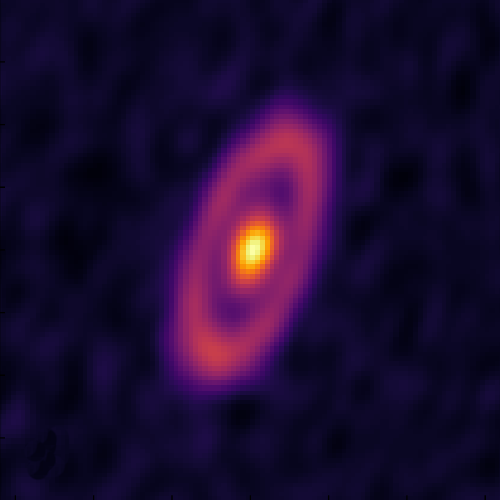
\includegraphics[interpolate=true,width=2.680000in,height=2.680000in]{images/fig3.2-img2.png}}%
\end{pgfscope}%
\begin{pgfscope}%
\pgfpathrectangle{\pgfqpoint{9.243828in}{0.515123in}}{\pgfqpoint{2.678922in}{2.678922in}}%
\pgfusepath{clip}%
\pgfsetbuttcap%
\pgfsetmiterjoin%
\definecolor{currentfill}{rgb}{0.501961,0.501961,0.501961}%
\pgfsetfillcolor{currentfill}%
\pgfsetlinewidth{1.003750pt}%
\definecolor{currentstroke}{rgb}{0.501961,0.501961,0.501961}%
\pgfsetstrokecolor{currentstroke}%
\pgfsetdash{}{0pt}%
\pgfpathmoveto{\pgfqpoint{9.620695in}{0.959407in}}%
\pgfpathcurveto{\pgfqpoint{9.641422in}{0.951450in}}{\pgfqpoint{9.656878in}{0.932290in}}{\pgfqpoint{9.663658in}{0.906145in}}%
\pgfpathcurveto{\pgfqpoint{9.670437in}{0.880000in}}{\pgfqpoint{9.667988in}{0.849005in}}{\pgfqpoint{9.656849in}{0.819987in}}%
\pgfpathcurveto{\pgfqpoint{9.645710in}{0.790969in}}{\pgfqpoint{9.626791in}{0.766297in}}{\pgfqpoint{9.604258in}{0.751404in}}%
\pgfpathcurveto{\pgfqpoint{9.581725in}{0.736511in}}{\pgfqpoint{9.557419in}{0.732614in}}{\pgfqpoint{9.536692in}{0.740570in}}%
\pgfpathcurveto{\pgfqpoint{9.515964in}{0.748527in}}{\pgfqpoint{9.500509in}{0.767687in}}{\pgfqpoint{9.493729in}{0.793832in}}%
\pgfpathcurveto{\pgfqpoint{9.486949in}{0.819977in}}{\pgfqpoint{9.489398in}{0.850972in}}{\pgfqpoint{9.500537in}{0.879990in}}%
\pgfpathcurveto{\pgfqpoint{9.511676in}{0.909008in}}{\pgfqpoint{9.530596in}{0.933680in}}{\pgfqpoint{9.553128in}{0.948573in}}%
\pgfpathcurveto{\pgfqpoint{9.575661in}{0.963466in}}{\pgfqpoint{9.599968in}{0.967363in}}{\pgfqpoint{9.620695in}{0.959407in}}%
\pgfpathclose%
\pgfusepath{stroke,fill}%
\end{pgfscope}%
\begin{pgfscope}%
\pgfsetbuttcap%
\pgfsetroundjoin%
\definecolor{currentfill}{rgb}{0.000000,0.000000,0.000000}%
\pgfsetfillcolor{currentfill}%
\pgfsetlinewidth{0.803000pt}%
\definecolor{currentstroke}{rgb}{0.000000,0.000000,0.000000}%
\pgfsetstrokecolor{currentstroke}%
\pgfsetdash{}{0pt}%
\pgfsys@defobject{currentmarker}{\pgfqpoint{0.000000in}{-0.048611in}}{\pgfqpoint{0.000000in}{0.000000in}}{%
\pgfpathmoveto{\pgfqpoint{0.000000in}{0.000000in}}%
\pgfpathlineto{\pgfqpoint{0.000000in}{-0.048611in}}%
\pgfusepath{stroke,fill}%
}%
\begin{pgfscope}%
\pgfsys@transformshift{11.420452in}{0.515123in}%
\pgfsys@useobject{currentmarker}{}%
\end{pgfscope}%
\end{pgfscope}%
\begin{pgfscope}%
\definecolor{textcolor}{rgb}{0.000000,0.000000,0.000000}%
\pgfsetstrokecolor{textcolor}%
\pgfsetfillcolor{textcolor}%
\pgftext[x=11.420452in,y=0.417901in,,top]{\color{textcolor}\rmfamily\fontsize{10.000000}{12.000000}\selectfont \(\displaystyle {\ensuremath{-}0.5}\)}%
\end{pgfscope}%
\begin{pgfscope}%
\pgfsetbuttcap%
\pgfsetroundjoin%
\definecolor{currentfill}{rgb}{0.000000,0.000000,0.000000}%
\pgfsetfillcolor{currentfill}%
\pgfsetlinewidth{0.803000pt}%
\definecolor{currentstroke}{rgb}{0.000000,0.000000,0.000000}%
\pgfsetstrokecolor{currentstroke}%
\pgfsetdash{}{0pt}%
\pgfsys@defobject{currentmarker}{\pgfqpoint{0.000000in}{-0.048611in}}{\pgfqpoint{0.000000in}{0.000000in}}{%
\pgfpathmoveto{\pgfqpoint{0.000000in}{0.000000in}}%
\pgfpathlineto{\pgfqpoint{0.000000in}{-0.048611in}}%
\pgfusepath{stroke,fill}%
}%
\begin{pgfscope}%
\pgfsys@transformshift{10.583289in}{0.515123in}%
\pgfsys@useobject{currentmarker}{}%
\end{pgfscope}%
\end{pgfscope}%
\begin{pgfscope}%
\definecolor{textcolor}{rgb}{0.000000,0.000000,0.000000}%
\pgfsetstrokecolor{textcolor}%
\pgfsetfillcolor{textcolor}%
\pgftext[x=10.583289in,y=0.417901in,,top]{\color{textcolor}\rmfamily\fontsize{10.000000}{12.000000}\selectfont \(\displaystyle {0.0}\)}%
\end{pgfscope}%
\begin{pgfscope}%
\pgfsetbuttcap%
\pgfsetroundjoin%
\definecolor{currentfill}{rgb}{0.000000,0.000000,0.000000}%
\pgfsetfillcolor{currentfill}%
\pgfsetlinewidth{0.803000pt}%
\definecolor{currentstroke}{rgb}{0.000000,0.000000,0.000000}%
\pgfsetstrokecolor{currentstroke}%
\pgfsetdash{}{0pt}%
\pgfsys@defobject{currentmarker}{\pgfqpoint{0.000000in}{-0.048611in}}{\pgfqpoint{0.000000in}{0.000000in}}{%
\pgfpathmoveto{\pgfqpoint{0.000000in}{0.000000in}}%
\pgfpathlineto{\pgfqpoint{0.000000in}{-0.048611in}}%
\pgfusepath{stroke,fill}%
}%
\begin{pgfscope}%
\pgfsys@transformshift{9.746126in}{0.515123in}%
\pgfsys@useobject{currentmarker}{}%
\end{pgfscope}%
\end{pgfscope}%
\begin{pgfscope}%
\definecolor{textcolor}{rgb}{0.000000,0.000000,0.000000}%
\pgfsetstrokecolor{textcolor}%
\pgfsetfillcolor{textcolor}%
\pgftext[x=9.746126in,y=0.417901in,,top]{\color{textcolor}\rmfamily\fontsize{10.000000}{12.000000}\selectfont \(\displaystyle {0.5}\)}%
\end{pgfscope}%
\begin{pgfscope}%
\definecolor{textcolor}{rgb}{0.000000,0.000000,0.000000}%
\pgfsetstrokecolor{textcolor}%
\pgfsetfillcolor{textcolor}%
\pgftext[x=10.583289in,y=0.238889in,,top]{\color{textcolor}\rmfamily\fontsize{10.000000}{12.000000}\selectfont \(\displaystyle \Delta RA [^\circ]\)}%
\end{pgfscope}%
\begin{pgfscope}%
\pgfsetbuttcap%
\pgfsetroundjoin%
\definecolor{currentfill}{rgb}{0.000000,0.000000,0.000000}%
\pgfsetfillcolor{currentfill}%
\pgfsetlinewidth{0.803000pt}%
\definecolor{currentstroke}{rgb}{0.000000,0.000000,0.000000}%
\pgfsetstrokecolor{currentstroke}%
\pgfsetdash{}{0pt}%
\pgfsys@defobject{currentmarker}{\pgfqpoint{-0.048611in}{0.000000in}}{\pgfqpoint{-0.000000in}{0.000000in}}{%
\pgfpathmoveto{\pgfqpoint{-0.000000in}{0.000000in}}%
\pgfpathlineto{\pgfqpoint{-0.048611in}{0.000000in}}%
\pgfusepath{stroke,fill}%
}%
\begin{pgfscope}%
\pgfsys@transformshift{9.243828in}{0.515123in}%
\pgfsys@useobject{currentmarker}{}%
\end{pgfscope}%
\end{pgfscope}%
\begin{pgfscope}%
\definecolor{textcolor}{rgb}{0.000000,0.000000,0.000000}%
\pgfsetstrokecolor{textcolor}%
\pgfsetfillcolor{textcolor}%
\pgftext[x=8.861111in, y=0.466898in, left, base]{\color{textcolor}\rmfamily\fontsize{10.000000}{12.000000}\selectfont \(\displaystyle {\ensuremath{-}0.8}\)}%
\end{pgfscope}%
\begin{pgfscope}%
\pgfsetbuttcap%
\pgfsetroundjoin%
\definecolor{currentfill}{rgb}{0.000000,0.000000,0.000000}%
\pgfsetfillcolor{currentfill}%
\pgfsetlinewidth{0.803000pt}%
\definecolor{currentstroke}{rgb}{0.000000,0.000000,0.000000}%
\pgfsetstrokecolor{currentstroke}%
\pgfsetdash{}{0pt}%
\pgfsys@defobject{currentmarker}{\pgfqpoint{-0.048611in}{0.000000in}}{\pgfqpoint{-0.000000in}{0.000000in}}{%
\pgfpathmoveto{\pgfqpoint{-0.000000in}{0.000000in}}%
\pgfpathlineto{\pgfqpoint{-0.048611in}{0.000000in}}%
\pgfusepath{stroke,fill}%
}%
\begin{pgfscope}%
\pgfsys@transformshift{9.243828in}{0.849989in}%
\pgfsys@useobject{currentmarker}{}%
\end{pgfscope}%
\end{pgfscope}%
\begin{pgfscope}%
\definecolor{textcolor}{rgb}{0.000000,0.000000,0.000000}%
\pgfsetstrokecolor{textcolor}%
\pgfsetfillcolor{textcolor}%
\pgftext[x=8.861111in, y=0.801763in, left, base]{\color{textcolor}\rmfamily\fontsize{10.000000}{12.000000}\selectfont \(\displaystyle {\ensuremath{-}0.6}\)}%
\end{pgfscope}%
\begin{pgfscope}%
\pgfsetbuttcap%
\pgfsetroundjoin%
\definecolor{currentfill}{rgb}{0.000000,0.000000,0.000000}%
\pgfsetfillcolor{currentfill}%
\pgfsetlinewidth{0.803000pt}%
\definecolor{currentstroke}{rgb}{0.000000,0.000000,0.000000}%
\pgfsetstrokecolor{currentstroke}%
\pgfsetdash{}{0pt}%
\pgfsys@defobject{currentmarker}{\pgfqpoint{-0.048611in}{0.000000in}}{\pgfqpoint{-0.000000in}{0.000000in}}{%
\pgfpathmoveto{\pgfqpoint{-0.000000in}{0.000000in}}%
\pgfpathlineto{\pgfqpoint{-0.048611in}{0.000000in}}%
\pgfusepath{stroke,fill}%
}%
\begin{pgfscope}%
\pgfsys@transformshift{9.243828in}{1.184854in}%
\pgfsys@useobject{currentmarker}{}%
\end{pgfscope}%
\end{pgfscope}%
\begin{pgfscope}%
\definecolor{textcolor}{rgb}{0.000000,0.000000,0.000000}%
\pgfsetstrokecolor{textcolor}%
\pgfsetfillcolor{textcolor}%
\pgftext[x=8.861111in, y=1.136629in, left, base]{\color{textcolor}\rmfamily\fontsize{10.000000}{12.000000}\selectfont \(\displaystyle {\ensuremath{-}0.4}\)}%
\end{pgfscope}%
\begin{pgfscope}%
\pgfsetbuttcap%
\pgfsetroundjoin%
\definecolor{currentfill}{rgb}{0.000000,0.000000,0.000000}%
\pgfsetfillcolor{currentfill}%
\pgfsetlinewidth{0.803000pt}%
\definecolor{currentstroke}{rgb}{0.000000,0.000000,0.000000}%
\pgfsetstrokecolor{currentstroke}%
\pgfsetdash{}{0pt}%
\pgfsys@defobject{currentmarker}{\pgfqpoint{-0.048611in}{0.000000in}}{\pgfqpoint{-0.000000in}{0.000000in}}{%
\pgfpathmoveto{\pgfqpoint{-0.000000in}{0.000000in}}%
\pgfpathlineto{\pgfqpoint{-0.048611in}{0.000000in}}%
\pgfusepath{stroke,fill}%
}%
\begin{pgfscope}%
\pgfsys@transformshift{9.243828in}{1.519719in}%
\pgfsys@useobject{currentmarker}{}%
\end{pgfscope}%
\end{pgfscope}%
\begin{pgfscope}%
\definecolor{textcolor}{rgb}{0.000000,0.000000,0.000000}%
\pgfsetstrokecolor{textcolor}%
\pgfsetfillcolor{textcolor}%
\pgftext[x=8.861111in, y=1.471494in, left, base]{\color{textcolor}\rmfamily\fontsize{10.000000}{12.000000}\selectfont \(\displaystyle {\ensuremath{-}0.2}\)}%
\end{pgfscope}%
\begin{pgfscope}%
\pgfsetbuttcap%
\pgfsetroundjoin%
\definecolor{currentfill}{rgb}{0.000000,0.000000,0.000000}%
\pgfsetfillcolor{currentfill}%
\pgfsetlinewidth{0.803000pt}%
\definecolor{currentstroke}{rgb}{0.000000,0.000000,0.000000}%
\pgfsetstrokecolor{currentstroke}%
\pgfsetdash{}{0pt}%
\pgfsys@defobject{currentmarker}{\pgfqpoint{-0.048611in}{0.000000in}}{\pgfqpoint{-0.000000in}{0.000000in}}{%
\pgfpathmoveto{\pgfqpoint{-0.000000in}{0.000000in}}%
\pgfpathlineto{\pgfqpoint{-0.048611in}{0.000000in}}%
\pgfusepath{stroke,fill}%
}%
\begin{pgfscope}%
\pgfsys@transformshift{9.243828in}{1.854584in}%
\pgfsys@useobject{currentmarker}{}%
\end{pgfscope}%
\end{pgfscope}%
\begin{pgfscope}%
\definecolor{textcolor}{rgb}{0.000000,0.000000,0.000000}%
\pgfsetstrokecolor{textcolor}%
\pgfsetfillcolor{textcolor}%
\pgftext[x=8.969136in, y=1.806359in, left, base]{\color{textcolor}\rmfamily\fontsize{10.000000}{12.000000}\selectfont \(\displaystyle {0.0}\)}%
\end{pgfscope}%
\begin{pgfscope}%
\pgfsetbuttcap%
\pgfsetroundjoin%
\definecolor{currentfill}{rgb}{0.000000,0.000000,0.000000}%
\pgfsetfillcolor{currentfill}%
\pgfsetlinewidth{0.803000pt}%
\definecolor{currentstroke}{rgb}{0.000000,0.000000,0.000000}%
\pgfsetstrokecolor{currentstroke}%
\pgfsetdash{}{0pt}%
\pgfsys@defobject{currentmarker}{\pgfqpoint{-0.048611in}{0.000000in}}{\pgfqpoint{-0.000000in}{0.000000in}}{%
\pgfpathmoveto{\pgfqpoint{-0.000000in}{0.000000in}}%
\pgfpathlineto{\pgfqpoint{-0.048611in}{0.000000in}}%
\pgfusepath{stroke,fill}%
}%
\begin{pgfscope}%
\pgfsys@transformshift{9.243828in}{2.189449in}%
\pgfsys@useobject{currentmarker}{}%
\end{pgfscope}%
\end{pgfscope}%
\begin{pgfscope}%
\definecolor{textcolor}{rgb}{0.000000,0.000000,0.000000}%
\pgfsetstrokecolor{textcolor}%
\pgfsetfillcolor{textcolor}%
\pgftext[x=8.969136in, y=2.141224in, left, base]{\color{textcolor}\rmfamily\fontsize{10.000000}{12.000000}\selectfont \(\displaystyle {0.2}\)}%
\end{pgfscope}%
\begin{pgfscope}%
\pgfsetbuttcap%
\pgfsetroundjoin%
\definecolor{currentfill}{rgb}{0.000000,0.000000,0.000000}%
\pgfsetfillcolor{currentfill}%
\pgfsetlinewidth{0.803000pt}%
\definecolor{currentstroke}{rgb}{0.000000,0.000000,0.000000}%
\pgfsetstrokecolor{currentstroke}%
\pgfsetdash{}{0pt}%
\pgfsys@defobject{currentmarker}{\pgfqpoint{-0.048611in}{0.000000in}}{\pgfqpoint{-0.000000in}{0.000000in}}{%
\pgfpathmoveto{\pgfqpoint{-0.000000in}{0.000000in}}%
\pgfpathlineto{\pgfqpoint{-0.048611in}{0.000000in}}%
\pgfusepath{stroke,fill}%
}%
\begin{pgfscope}%
\pgfsys@transformshift{9.243828in}{2.524315in}%
\pgfsys@useobject{currentmarker}{}%
\end{pgfscope}%
\end{pgfscope}%
\begin{pgfscope}%
\definecolor{textcolor}{rgb}{0.000000,0.000000,0.000000}%
\pgfsetstrokecolor{textcolor}%
\pgfsetfillcolor{textcolor}%
\pgftext[x=8.969136in, y=2.476089in, left, base]{\color{textcolor}\rmfamily\fontsize{10.000000}{12.000000}\selectfont \(\displaystyle {0.4}\)}%
\end{pgfscope}%
\begin{pgfscope}%
\pgfsetbuttcap%
\pgfsetroundjoin%
\definecolor{currentfill}{rgb}{0.000000,0.000000,0.000000}%
\pgfsetfillcolor{currentfill}%
\pgfsetlinewidth{0.803000pt}%
\definecolor{currentstroke}{rgb}{0.000000,0.000000,0.000000}%
\pgfsetstrokecolor{currentstroke}%
\pgfsetdash{}{0pt}%
\pgfsys@defobject{currentmarker}{\pgfqpoint{-0.048611in}{0.000000in}}{\pgfqpoint{-0.000000in}{0.000000in}}{%
\pgfpathmoveto{\pgfqpoint{-0.000000in}{0.000000in}}%
\pgfpathlineto{\pgfqpoint{-0.048611in}{0.000000in}}%
\pgfusepath{stroke,fill}%
}%
\begin{pgfscope}%
\pgfsys@transformshift{9.243828in}{2.859180in}%
\pgfsys@useobject{currentmarker}{}%
\end{pgfscope}%
\end{pgfscope}%
\begin{pgfscope}%
\definecolor{textcolor}{rgb}{0.000000,0.000000,0.000000}%
\pgfsetstrokecolor{textcolor}%
\pgfsetfillcolor{textcolor}%
\pgftext[x=8.969136in, y=2.810955in, left, base]{\color{textcolor}\rmfamily\fontsize{10.000000}{12.000000}\selectfont \(\displaystyle {0.6}\)}%
\end{pgfscope}%
\begin{pgfscope}%
\pgfsetbuttcap%
\pgfsetroundjoin%
\definecolor{currentfill}{rgb}{0.000000,0.000000,0.000000}%
\pgfsetfillcolor{currentfill}%
\pgfsetlinewidth{0.803000pt}%
\definecolor{currentstroke}{rgb}{0.000000,0.000000,0.000000}%
\pgfsetstrokecolor{currentstroke}%
\pgfsetdash{}{0pt}%
\pgfsys@defobject{currentmarker}{\pgfqpoint{-0.048611in}{0.000000in}}{\pgfqpoint{-0.000000in}{0.000000in}}{%
\pgfpathmoveto{\pgfqpoint{-0.000000in}{0.000000in}}%
\pgfpathlineto{\pgfqpoint{-0.048611in}{0.000000in}}%
\pgfusepath{stroke,fill}%
}%
\begin{pgfscope}%
\pgfsys@transformshift{9.243828in}{3.194045in}%
\pgfsys@useobject{currentmarker}{}%
\end{pgfscope}%
\end{pgfscope}%
\begin{pgfscope}%
\definecolor{textcolor}{rgb}{0.000000,0.000000,0.000000}%
\pgfsetstrokecolor{textcolor}%
\pgfsetfillcolor{textcolor}%
\pgftext[x=8.969136in, y=3.145820in, left, base]{\color{textcolor}\rmfamily\fontsize{10.000000}{12.000000}\selectfont \(\displaystyle {0.8}\)}%
\end{pgfscope}%
\begin{pgfscope}%
\definecolor{textcolor}{rgb}{0.000000,0.000000,0.000000}%
\pgfsetstrokecolor{textcolor}%
\pgfsetfillcolor{textcolor}%
\pgftext[x=8.805556in,y=1.854584in,,bottom,rotate=90.000000]{\color{textcolor}\rmfamily\fontsize{10.000000}{12.000000}\selectfont \(\displaystyle \Delta Dec [^\circ]\)}%
\end{pgfscope}%
\begin{pgfscope}%
\pgfsetrectcap%
\pgfsetmiterjoin%
\pgfsetlinewidth{0.803000pt}%
\definecolor{currentstroke}{rgb}{0.000000,0.000000,0.000000}%
\pgfsetstrokecolor{currentstroke}%
\pgfsetdash{}{0pt}%
\pgfpathmoveto{\pgfqpoint{9.243828in}{0.515123in}}%
\pgfpathlineto{\pgfqpoint{9.243828in}{3.194045in}}%
\pgfusepath{stroke}%
\end{pgfscope}%
\begin{pgfscope}%
\pgfsetrectcap%
\pgfsetmiterjoin%
\pgfsetlinewidth{0.803000pt}%
\definecolor{currentstroke}{rgb}{0.000000,0.000000,0.000000}%
\pgfsetstrokecolor{currentstroke}%
\pgfsetdash{}{0pt}%
\pgfpathmoveto{\pgfqpoint{11.922750in}{0.515123in}}%
\pgfpathlineto{\pgfqpoint{11.922750in}{3.194045in}}%
\pgfusepath{stroke}%
\end{pgfscope}%
\begin{pgfscope}%
\pgfsetrectcap%
\pgfsetmiterjoin%
\pgfsetlinewidth{0.803000pt}%
\definecolor{currentstroke}{rgb}{0.000000,0.000000,0.000000}%
\pgfsetstrokecolor{currentstroke}%
\pgfsetdash{}{0pt}%
\pgfpathmoveto{\pgfqpoint{9.243828in}{0.515123in}}%
\pgfpathlineto{\pgfqpoint{11.922750in}{0.515123in}}%
\pgfusepath{stroke}%
\end{pgfscope}%
\begin{pgfscope}%
\pgfsetrectcap%
\pgfsetmiterjoin%
\pgfsetlinewidth{0.803000pt}%
\definecolor{currentstroke}{rgb}{0.000000,0.000000,0.000000}%
\pgfsetstrokecolor{currentstroke}%
\pgfsetdash{}{0pt}%
\pgfpathmoveto{\pgfqpoint{9.243828in}{3.194045in}}%
\pgfpathlineto{\pgfqpoint{11.922750in}{3.194045in}}%
\pgfusepath{stroke}%
\end{pgfscope}%
\begin{pgfscope}%
\pgfsetbuttcap%
\pgfsetmiterjoin%
\definecolor{currentfill}{rgb}{1.000000,1.000000,1.000000}%
\pgfsetfillcolor{currentfill}%
\pgfsetlinewidth{0.000000pt}%
\definecolor{currentstroke}{rgb}{0.000000,0.000000,0.000000}%
\pgfsetstrokecolor{currentstroke}%
\pgfsetstrokeopacity{0.000000}%
\pgfsetdash{}{0pt}%
\pgfpathmoveto{\pgfqpoint{7.689417in}{0.515123in}}%
\pgfpathlineto{\pgfqpoint{7.823363in}{0.515123in}}%
\pgfpathlineto{\pgfqpoint{7.823363in}{3.194045in}}%
\pgfpathlineto{\pgfqpoint{7.689417in}{3.194045in}}%
\pgfpathclose%
\pgfusepath{fill}%
\end{pgfscope}%
\begin{pgfscope}%
\pgfpathrectangle{\pgfqpoint{7.689417in}{0.515123in}}{\pgfqpoint{0.133946in}{2.678922in}}%
\pgfusepath{clip}%
\pgfsetbuttcap%
\pgfsetmiterjoin%
\definecolor{currentfill}{rgb}{1.000000,1.000000,1.000000}%
\pgfsetfillcolor{currentfill}%
\pgfsetlinewidth{0.010037pt}%
\definecolor{currentstroke}{rgb}{1.000000,1.000000,1.000000}%
\pgfsetstrokecolor{currentstroke}%
\pgfsetdash{}{0pt}%
\pgfpathmoveto{\pgfqpoint{7.689417in}{0.515123in}}%
\pgfpathlineto{\pgfqpoint{7.689417in}{0.525588in}}%
\pgfpathlineto{\pgfqpoint{7.689417in}{3.183581in}}%
\pgfpathlineto{\pgfqpoint{7.689417in}{3.194045in}}%
\pgfpathlineto{\pgfqpoint{7.823363in}{3.194045in}}%
\pgfpathlineto{\pgfqpoint{7.823363in}{3.183581in}}%
\pgfpathlineto{\pgfqpoint{7.823363in}{0.525588in}}%
\pgfpathlineto{\pgfqpoint{7.823363in}{0.515123in}}%
\pgfpathlineto{\pgfqpoint{7.823363in}{0.515123in}}%
\pgfpathclose%
\pgfusepath{stroke,fill}%
\end{pgfscope}%
\begin{pgfscope}%
\pgfsys@transformshift{7.690000in}{0.515280in}%
\pgftext[left,bottom]{
\includegraphics[interpolate=true,width=0.132500in,height=2.680000in]{images/fig3.2-img3.png}}%
\end{pgfscope}%
\begin{pgfscope}%
\pgfsetbuttcap%
\pgfsetroundjoin%
\definecolor{currentfill}{rgb}{0.000000,0.000000,0.000000}%
\pgfsetfillcolor{currentfill}%
\pgfsetlinewidth{0.803000pt}%
\definecolor{currentstroke}{rgb}{0.000000,0.000000,0.000000}%
\pgfsetstrokecolor{currentstroke}%
\pgfsetdash{}{0pt}%
\pgfsys@defobject{currentmarker}{\pgfqpoint{0.000000in}{0.000000in}}{\pgfqpoint{0.048611in}{0.000000in}}{%
\pgfpathmoveto{\pgfqpoint{0.000000in}{0.000000in}}%
\pgfpathlineto{\pgfqpoint{0.048611in}{0.000000in}}%
\pgfusepath{stroke,fill}%
}%
\begin{pgfscope}%
\pgfsys@transformshift{7.823363in}{0.961610in}%
\pgfsys@useobject{currentmarker}{}%
\end{pgfscope}%
\end{pgfscope}%
\begin{pgfscope}%
\definecolor{textcolor}{rgb}{0.000000,0.000000,0.000000}%
\pgfsetstrokecolor{textcolor}%
\pgfsetfillcolor{textcolor}%
\pgftext[x=7.920585in, y=0.913385in, left, base]{\color{textcolor}\rmfamily\fontsize{10.000000}{12.000000}\selectfont \(\displaystyle {0.0005}\)}%
\end{pgfscope}%
\begin{pgfscope}%
\pgfsetbuttcap%
\pgfsetroundjoin%
\definecolor{currentfill}{rgb}{0.000000,0.000000,0.000000}%
\pgfsetfillcolor{currentfill}%
\pgfsetlinewidth{0.803000pt}%
\definecolor{currentstroke}{rgb}{0.000000,0.000000,0.000000}%
\pgfsetstrokecolor{currentstroke}%
\pgfsetdash{}{0pt}%
\pgfsys@defobject{currentmarker}{\pgfqpoint{0.000000in}{0.000000in}}{\pgfqpoint{0.048611in}{0.000000in}}{%
\pgfpathmoveto{\pgfqpoint{0.000000in}{0.000000in}}%
\pgfpathlineto{\pgfqpoint{0.048611in}{0.000000in}}%
\pgfusepath{stroke,fill}%
}%
\begin{pgfscope}%
\pgfsys@transformshift{7.823363in}{1.408097in}%
\pgfsys@useobject{currentmarker}{}%
\end{pgfscope}%
\end{pgfscope}%
\begin{pgfscope}%
\definecolor{textcolor}{rgb}{0.000000,0.000000,0.000000}%
\pgfsetstrokecolor{textcolor}%
\pgfsetfillcolor{textcolor}%
\pgftext[x=7.920585in, y=1.359872in, left, base]{\color{textcolor}\rmfamily\fontsize{10.000000}{12.000000}\selectfont \(\displaystyle {0.0010}\)}%
\end{pgfscope}%
\begin{pgfscope}%
\pgfsetbuttcap%
\pgfsetroundjoin%
\definecolor{currentfill}{rgb}{0.000000,0.000000,0.000000}%
\pgfsetfillcolor{currentfill}%
\pgfsetlinewidth{0.803000pt}%
\definecolor{currentstroke}{rgb}{0.000000,0.000000,0.000000}%
\pgfsetstrokecolor{currentstroke}%
\pgfsetdash{}{0pt}%
\pgfsys@defobject{currentmarker}{\pgfqpoint{0.000000in}{0.000000in}}{\pgfqpoint{0.048611in}{0.000000in}}{%
\pgfpathmoveto{\pgfqpoint{0.000000in}{0.000000in}}%
\pgfpathlineto{\pgfqpoint{0.048611in}{0.000000in}}%
\pgfusepath{stroke,fill}%
}%
\begin{pgfscope}%
\pgfsys@transformshift{7.823363in}{1.854584in}%
\pgfsys@useobject{currentmarker}{}%
\end{pgfscope}%
\end{pgfscope}%
\begin{pgfscope}%
\definecolor{textcolor}{rgb}{0.000000,0.000000,0.000000}%
\pgfsetstrokecolor{textcolor}%
\pgfsetfillcolor{textcolor}%
\pgftext[x=7.920585in, y=1.806359in, left, base]{\color{textcolor}\rmfamily\fontsize{10.000000}{12.000000}\selectfont \(\displaystyle {0.0015}\)}%
\end{pgfscope}%
\begin{pgfscope}%
\pgfsetbuttcap%
\pgfsetroundjoin%
\definecolor{currentfill}{rgb}{0.000000,0.000000,0.000000}%
\pgfsetfillcolor{currentfill}%
\pgfsetlinewidth{0.803000pt}%
\definecolor{currentstroke}{rgb}{0.000000,0.000000,0.000000}%
\pgfsetstrokecolor{currentstroke}%
\pgfsetdash{}{0pt}%
\pgfsys@defobject{currentmarker}{\pgfqpoint{0.000000in}{0.000000in}}{\pgfqpoint{0.048611in}{0.000000in}}{%
\pgfpathmoveto{\pgfqpoint{0.000000in}{0.000000in}}%
\pgfpathlineto{\pgfqpoint{0.048611in}{0.000000in}}%
\pgfusepath{stroke,fill}%
}%
\begin{pgfscope}%
\pgfsys@transformshift{7.823363in}{2.301071in}%
\pgfsys@useobject{currentmarker}{}%
\end{pgfscope}%
\end{pgfscope}%
\begin{pgfscope}%
\definecolor{textcolor}{rgb}{0.000000,0.000000,0.000000}%
\pgfsetstrokecolor{textcolor}%
\pgfsetfillcolor{textcolor}%
\pgftext[x=7.920585in, y=2.252846in, left, base]{\color{textcolor}\rmfamily\fontsize{10.000000}{12.000000}\selectfont \(\displaystyle {0.0020}\)}%
\end{pgfscope}%
\begin{pgfscope}%
\pgfsetbuttcap%
\pgfsetroundjoin%
\definecolor{currentfill}{rgb}{0.000000,0.000000,0.000000}%
\pgfsetfillcolor{currentfill}%
\pgfsetlinewidth{0.803000pt}%
\definecolor{currentstroke}{rgb}{0.000000,0.000000,0.000000}%
\pgfsetstrokecolor{currentstroke}%
\pgfsetdash{}{0pt}%
\pgfsys@defobject{currentmarker}{\pgfqpoint{0.000000in}{0.000000in}}{\pgfqpoint{0.048611in}{0.000000in}}{%
\pgfpathmoveto{\pgfqpoint{0.000000in}{0.000000in}}%
\pgfpathlineto{\pgfqpoint{0.048611in}{0.000000in}}%
\pgfusepath{stroke,fill}%
}%
\begin{pgfscope}%
\pgfsys@transformshift{7.823363in}{2.747558in}%
\pgfsys@useobject{currentmarker}{}%
\end{pgfscope}%
\end{pgfscope}%
\begin{pgfscope}%
\definecolor{textcolor}{rgb}{0.000000,0.000000,0.000000}%
\pgfsetstrokecolor{textcolor}%
\pgfsetfillcolor{textcolor}%
\pgftext[x=7.920585in, y=2.699333in, left, base]{\color{textcolor}\rmfamily\fontsize{10.000000}{12.000000}\selectfont \(\displaystyle {0.0025}\)}%
\end{pgfscope}%
\begin{pgfscope}%
\pgfsetbuttcap%
\pgfsetroundjoin%
\definecolor{currentfill}{rgb}{0.000000,0.000000,0.000000}%
\pgfsetfillcolor{currentfill}%
\pgfsetlinewidth{0.803000pt}%
\definecolor{currentstroke}{rgb}{0.000000,0.000000,0.000000}%
\pgfsetstrokecolor{currentstroke}%
\pgfsetdash{}{0pt}%
\pgfsys@defobject{currentmarker}{\pgfqpoint{0.000000in}{0.000000in}}{\pgfqpoint{0.048611in}{0.000000in}}{%
\pgfpathmoveto{\pgfqpoint{0.000000in}{0.000000in}}%
\pgfpathlineto{\pgfqpoint{0.048611in}{0.000000in}}%
\pgfusepath{stroke,fill}%
}%
\begin{pgfscope}%
\pgfsys@transformshift{7.823363in}{3.194045in}%
\pgfsys@useobject{currentmarker}{}%
\end{pgfscope}%
\end{pgfscope}%
\begin{pgfscope}%
\definecolor{textcolor}{rgb}{0.000000,0.000000,0.000000}%
\pgfsetstrokecolor{textcolor}%
\pgfsetfillcolor{textcolor}%
\pgftext[x=7.920585in, y=3.145820in, left, base]{\color{textcolor}\rmfamily\fontsize{10.000000}{12.000000}\selectfont \(\displaystyle {0.0030}\)}%
\end{pgfscope}%
\begin{pgfscope}%
\definecolor{textcolor}{rgb}{0.000000,0.000000,0.000000}%
\pgfsetstrokecolor{textcolor}%
\pgfsetfillcolor{textcolor}%
\pgftext[x=8.361944in,y=1.854584in,,top,rotate=90.000000]{\color{textcolor}\rmfamily\fontsize{10.000000}{12.000000}\selectfont Flux density [Jy.beam\(\displaystyle ^{-1}\)]}%
\end{pgfscope}%
\begin{pgfscope}%
\pgfsetrectcap%
\pgfsetmiterjoin%
\pgfsetlinewidth{0.803000pt}%
\definecolor{currentstroke}{rgb}{0.000000,0.000000,0.000000}%
\pgfsetstrokecolor{currentstroke}%
\pgfsetdash{}{0pt}%
\pgfpathmoveto{\pgfqpoint{7.689417in}{0.515123in}}%
\pgfpathlineto{\pgfqpoint{7.689417in}{0.525588in}}%
\pgfpathlineto{\pgfqpoint{7.689417in}{3.183581in}}%
\pgfpathlineto{\pgfqpoint{7.689417in}{3.194045in}}%
\pgfpathlineto{\pgfqpoint{7.823363in}{3.194045in}}%
\pgfpathlineto{\pgfqpoint{7.823363in}{3.183581in}}%
\pgfpathlineto{\pgfqpoint{7.823363in}{0.525588in}}%
\pgfpathlineto{\pgfqpoint{7.823363in}{0.515123in}}%
\pgfpathclose%
\pgfusepath{stroke}%
\end{pgfscope}%
\begin{pgfscope}%
\pgfsetbuttcap%
\pgfsetmiterjoin%
\definecolor{currentfill}{rgb}{1.000000,1.000000,1.000000}%
\pgfsetfillcolor{currentfill}%
\pgfsetlinewidth{0.000000pt}%
\definecolor{currentstroke}{rgb}{0.000000,0.000000,0.000000}%
\pgfsetstrokecolor{currentstroke}%
\pgfsetstrokeopacity{0.000000}%
\pgfsetdash{}{0pt}%
\pgfpathmoveto{\pgfqpoint{3.406083in}{0.515123in}}%
\pgfpathlineto{\pgfqpoint{3.540029in}{0.515123in}}%
\pgfpathlineto{\pgfqpoint{3.540029in}{3.194045in}}%
\pgfpathlineto{\pgfqpoint{3.406083in}{3.194045in}}%
\pgfpathclose%
\pgfusepath{fill}%
\end{pgfscope}%
\begin{pgfscope}%
\pgfpathrectangle{\pgfqpoint{3.406083in}{0.515123in}}{\pgfqpoint{0.133946in}{2.678922in}}%
\pgfusepath{clip}%
\pgfsetbuttcap%
\pgfsetmiterjoin%
\definecolor{currentfill}{rgb}{1.000000,1.000000,1.000000}%
\pgfsetfillcolor{currentfill}%
\pgfsetlinewidth{0.010037pt}%
\definecolor{currentstroke}{rgb}{1.000000,1.000000,1.000000}%
\pgfsetstrokecolor{currentstroke}%
\pgfsetdash{}{0pt}%
\pgfpathmoveto{\pgfqpoint{3.406083in}{0.515123in}}%
\pgfpathlineto{\pgfqpoint{3.406083in}{0.525588in}}%
\pgfpathlineto{\pgfqpoint{3.406083in}{3.183581in}}%
\pgfpathlineto{\pgfqpoint{3.406083in}{3.194045in}}%
\pgfpathlineto{\pgfqpoint{3.540029in}{3.194045in}}%
\pgfpathlineto{\pgfqpoint{3.540029in}{3.183581in}}%
\pgfpathlineto{\pgfqpoint{3.540029in}{0.525588in}}%
\pgfpathlineto{\pgfqpoint{3.540029in}{0.515123in}}%
\pgfpathlineto{\pgfqpoint{3.540029in}{0.515123in}}%
\pgfpathclose%
\pgfusepath{stroke,fill}%
\end{pgfscope}%
\begin{pgfscope}%
\pgfsys@transformshift{3.405000in}{0.515280in}%
\pgftext[left,bottom]{
\includegraphics[interpolate=true,width=0.135000in,height=2.680000in]{images/fig3.2-img4.png}}%
\end{pgfscope}%
\begin{pgfscope}%
\pgfsetbuttcap%
\pgfsetroundjoin%
\definecolor{currentfill}{rgb}{0.000000,0.000000,0.000000}%
\pgfsetfillcolor{currentfill}%
\pgfsetlinewidth{0.803000pt}%
\definecolor{currentstroke}{rgb}{0.000000,0.000000,0.000000}%
\pgfsetstrokecolor{currentstroke}%
\pgfsetdash{}{0pt}%
\pgfsys@defobject{currentmarker}{\pgfqpoint{0.000000in}{0.000000in}}{\pgfqpoint{0.048611in}{0.000000in}}{%
\pgfpathmoveto{\pgfqpoint{0.000000in}{0.000000in}}%
\pgfpathlineto{\pgfqpoint{0.048611in}{0.000000in}}%
\pgfusepath{stroke,fill}%
}%
\begin{pgfscope}%
\pgfsys@transformshift{3.540029in}{0.515123in}%
\pgfsys@useobject{currentmarker}{}%
\end{pgfscope}%
\end{pgfscope}%
\begin{pgfscope}%
\definecolor{textcolor}{rgb}{0.000000,0.000000,0.000000}%
\pgfsetstrokecolor{textcolor}%
\pgfsetfillcolor{textcolor}%
\pgftext[x=3.637252in, y=0.466898in, left, base]{\color{textcolor}\rmfamily\fontsize{10.000000}{12.000000}\selectfont \(\displaystyle {0.0}\)}%
\end{pgfscope}%
\begin{pgfscope}%
\pgfsetbuttcap%
\pgfsetroundjoin%
\definecolor{currentfill}{rgb}{0.000000,0.000000,0.000000}%
\pgfsetfillcolor{currentfill}%
\pgfsetlinewidth{0.803000pt}%
\definecolor{currentstroke}{rgb}{0.000000,0.000000,0.000000}%
\pgfsetstrokecolor{currentstroke}%
\pgfsetdash{}{0pt}%
\pgfsys@defobject{currentmarker}{\pgfqpoint{0.000000in}{0.000000in}}{\pgfqpoint{0.048611in}{0.000000in}}{%
\pgfpathmoveto{\pgfqpoint{0.000000in}{0.000000in}}%
\pgfpathlineto{\pgfqpoint{0.048611in}{0.000000in}}%
\pgfusepath{stroke,fill}%
}%
\begin{pgfscope}%
\pgfsys@transformshift{3.540029in}{0.914812in}%
\pgfsys@useobject{currentmarker}{}%
\end{pgfscope}%
\end{pgfscope}%
\begin{pgfscope}%
\definecolor{textcolor}{rgb}{0.000000,0.000000,0.000000}%
\pgfsetstrokecolor{textcolor}%
\pgfsetfillcolor{textcolor}%
\pgftext[x=3.637252in, y=0.866587in, left, base]{\color{textcolor}\rmfamily\fontsize{10.000000}{12.000000}\selectfont \(\displaystyle {0.2}\)}%
\end{pgfscope}%
\begin{pgfscope}%
\pgfsetbuttcap%
\pgfsetroundjoin%
\definecolor{currentfill}{rgb}{0.000000,0.000000,0.000000}%
\pgfsetfillcolor{currentfill}%
\pgfsetlinewidth{0.803000pt}%
\definecolor{currentstroke}{rgb}{0.000000,0.000000,0.000000}%
\pgfsetstrokecolor{currentstroke}%
\pgfsetdash{}{0pt}%
\pgfsys@defobject{currentmarker}{\pgfqpoint{0.000000in}{0.000000in}}{\pgfqpoint{0.048611in}{0.000000in}}{%
\pgfpathmoveto{\pgfqpoint{0.000000in}{0.000000in}}%
\pgfpathlineto{\pgfqpoint{0.048611in}{0.000000in}}%
\pgfusepath{stroke,fill}%
}%
\begin{pgfscope}%
\pgfsys@transformshift{3.540029in}{1.314501in}%
\pgfsys@useobject{currentmarker}{}%
\end{pgfscope}%
\end{pgfscope}%
\begin{pgfscope}%
\definecolor{textcolor}{rgb}{0.000000,0.000000,0.000000}%
\pgfsetstrokecolor{textcolor}%
\pgfsetfillcolor{textcolor}%
\pgftext[x=3.637252in, y=1.266276in, left, base]{\color{textcolor}\rmfamily\fontsize{10.000000}{12.000000}\selectfont \(\displaystyle {0.4}\)}%
\end{pgfscope}%
\begin{pgfscope}%
\pgfsetbuttcap%
\pgfsetroundjoin%
\definecolor{currentfill}{rgb}{0.000000,0.000000,0.000000}%
\pgfsetfillcolor{currentfill}%
\pgfsetlinewidth{0.803000pt}%
\definecolor{currentstroke}{rgb}{0.000000,0.000000,0.000000}%
\pgfsetstrokecolor{currentstroke}%
\pgfsetdash{}{0pt}%
\pgfsys@defobject{currentmarker}{\pgfqpoint{0.000000in}{0.000000in}}{\pgfqpoint{0.048611in}{0.000000in}}{%
\pgfpathmoveto{\pgfqpoint{0.000000in}{0.000000in}}%
\pgfpathlineto{\pgfqpoint{0.048611in}{0.000000in}}%
\pgfusepath{stroke,fill}%
}%
\begin{pgfscope}%
\pgfsys@transformshift{3.540029in}{1.714190in}%
\pgfsys@useobject{currentmarker}{}%
\end{pgfscope}%
\end{pgfscope}%
\begin{pgfscope}%
\definecolor{textcolor}{rgb}{0.000000,0.000000,0.000000}%
\pgfsetstrokecolor{textcolor}%
\pgfsetfillcolor{textcolor}%
\pgftext[x=3.637252in, y=1.665964in, left, base]{\color{textcolor}\rmfamily\fontsize{10.000000}{12.000000}\selectfont \(\displaystyle {0.6}\)}%
\end{pgfscope}%
\begin{pgfscope}%
\pgfsetbuttcap%
\pgfsetroundjoin%
\definecolor{currentfill}{rgb}{0.000000,0.000000,0.000000}%
\pgfsetfillcolor{currentfill}%
\pgfsetlinewidth{0.803000pt}%
\definecolor{currentstroke}{rgb}{0.000000,0.000000,0.000000}%
\pgfsetstrokecolor{currentstroke}%
\pgfsetdash{}{0pt}%
\pgfsys@defobject{currentmarker}{\pgfqpoint{0.000000in}{0.000000in}}{\pgfqpoint{0.048611in}{0.000000in}}{%
\pgfpathmoveto{\pgfqpoint{0.000000in}{0.000000in}}%
\pgfpathlineto{\pgfqpoint{0.048611in}{0.000000in}}%
\pgfusepath{stroke,fill}%
}%
\begin{pgfscope}%
\pgfsys@transformshift{3.540029in}{2.113878in}%
\pgfsys@useobject{currentmarker}{}%
\end{pgfscope}%
\end{pgfscope}%
\begin{pgfscope}%
\definecolor{textcolor}{rgb}{0.000000,0.000000,0.000000}%
\pgfsetstrokecolor{textcolor}%
\pgfsetfillcolor{textcolor}%
\pgftext[x=3.637252in, y=2.065653in, left, base]{\color{textcolor}\rmfamily\fontsize{10.000000}{12.000000}\selectfont \(\displaystyle {0.8}\)}%
\end{pgfscope}%
\begin{pgfscope}%
\pgfsetbuttcap%
\pgfsetroundjoin%
\definecolor{currentfill}{rgb}{0.000000,0.000000,0.000000}%
\pgfsetfillcolor{currentfill}%
\pgfsetlinewidth{0.803000pt}%
\definecolor{currentstroke}{rgb}{0.000000,0.000000,0.000000}%
\pgfsetstrokecolor{currentstroke}%
\pgfsetdash{}{0pt}%
\pgfsys@defobject{currentmarker}{\pgfqpoint{0.000000in}{0.000000in}}{\pgfqpoint{0.048611in}{0.000000in}}{%
\pgfpathmoveto{\pgfqpoint{0.000000in}{0.000000in}}%
\pgfpathlineto{\pgfqpoint{0.048611in}{0.000000in}}%
\pgfusepath{stroke,fill}%
}%
\begin{pgfscope}%
\pgfsys@transformshift{3.540029in}{2.513567in}%
\pgfsys@useobject{currentmarker}{}%
\end{pgfscope}%
\end{pgfscope}%
\begin{pgfscope}%
\definecolor{textcolor}{rgb}{0.000000,0.000000,0.000000}%
\pgfsetstrokecolor{textcolor}%
\pgfsetfillcolor{textcolor}%
\pgftext[x=3.637252in, y=2.465342in, left, base]{\color{textcolor}\rmfamily\fontsize{10.000000}{12.000000}\selectfont \(\displaystyle {1.0}\)}%
\end{pgfscope}%
\begin{pgfscope}%
\pgfsetbuttcap%
\pgfsetroundjoin%
\definecolor{currentfill}{rgb}{0.000000,0.000000,0.000000}%
\pgfsetfillcolor{currentfill}%
\pgfsetlinewidth{0.803000pt}%
\definecolor{currentstroke}{rgb}{0.000000,0.000000,0.000000}%
\pgfsetstrokecolor{currentstroke}%
\pgfsetdash{}{0pt}%
\pgfsys@defobject{currentmarker}{\pgfqpoint{0.000000in}{0.000000in}}{\pgfqpoint{0.048611in}{0.000000in}}{%
\pgfpathmoveto{\pgfqpoint{0.000000in}{0.000000in}}%
\pgfpathlineto{\pgfqpoint{0.048611in}{0.000000in}}%
\pgfusepath{stroke,fill}%
}%
\begin{pgfscope}%
\pgfsys@transformshift{3.540029in}{2.913256in}%
\pgfsys@useobject{currentmarker}{}%
\end{pgfscope}%
\end{pgfscope}%
\begin{pgfscope}%
\definecolor{textcolor}{rgb}{0.000000,0.000000,0.000000}%
\pgfsetstrokecolor{textcolor}%
\pgfsetfillcolor{textcolor}%
\pgftext[x=3.637252in, y=2.865031in, left, base]{\color{textcolor}\rmfamily\fontsize{10.000000}{12.000000}\selectfont \(\displaystyle {1.2}\)}%
\end{pgfscope}%
\begin{pgfscope}%
\definecolor{textcolor}{rgb}{0.000000,0.000000,0.000000}%
\pgfsetstrokecolor{textcolor}%
\pgfsetfillcolor{textcolor}%
\pgftext[x=3.870277in,y=1.854584in,,top,rotate=90.000000]{\color{textcolor}\rmfamily\fontsize{10.000000}{12.000000}\selectfont Flux density [Jy.beam\(\displaystyle ^{-1}\)]}%
\end{pgfscope}%
\begin{pgfscope}%
\definecolor{textcolor}{rgb}{0.000000,0.000000,0.000000}%
\pgfsetstrokecolor{textcolor}%
\pgfsetfillcolor{textcolor}%
\pgftext[x=3.540029in,y=3.235712in,right,base]{\color{textcolor}\rmfamily\fontsize{10.000000}{12.000000}\selectfont \(\displaystyle \times{10^{\ensuremath{-}10}}{}\)}%
\end{pgfscope}%
\begin{pgfscope}%
\pgfsetrectcap%
\pgfsetmiterjoin%
\pgfsetlinewidth{0.803000pt}%
\definecolor{currentstroke}{rgb}{0.000000,0.000000,0.000000}%
\pgfsetstrokecolor{currentstroke}%
\pgfsetdash{}{0pt}%
\pgfpathmoveto{\pgfqpoint{3.406083in}{0.515123in}}%
\pgfpathlineto{\pgfqpoint{3.406083in}{0.525588in}}%
\pgfpathlineto{\pgfqpoint{3.406083in}{3.183581in}}%
\pgfpathlineto{\pgfqpoint{3.406083in}{3.194045in}}%
\pgfpathlineto{\pgfqpoint{3.540029in}{3.194045in}}%
\pgfpathlineto{\pgfqpoint{3.540029in}{3.183581in}}%
\pgfpathlineto{\pgfqpoint{3.540029in}{0.525588in}}%
\pgfpathlineto{\pgfqpoint{3.540029in}{0.515123in}}%
\pgfpathclose%
\pgfusepath{stroke}%
\end{pgfscope}%
\begin{pgfscope}%
\pgfsetbuttcap%
\pgfsetmiterjoin%
\definecolor{currentfill}{rgb}{1.000000,1.000000,1.000000}%
\pgfsetfillcolor{currentfill}%
\pgfsetlinewidth{0.000000pt}%
\definecolor{currentstroke}{rgb}{0.000000,0.000000,0.000000}%
\pgfsetstrokecolor{currentstroke}%
\pgfsetstrokeopacity{0.000000}%
\pgfsetdash{}{0pt}%
\pgfpathmoveto{\pgfqpoint{11.972750in}{0.515123in}}%
\pgfpathlineto{\pgfqpoint{12.106696in}{0.515123in}}%
\pgfpathlineto{\pgfqpoint{12.106696in}{3.194045in}}%
\pgfpathlineto{\pgfqpoint{11.972750in}{3.194045in}}%
\pgfpathclose%
\pgfusepath{fill}%
\end{pgfscope}%
\begin{pgfscope}%
\pgfpathrectangle{\pgfqpoint{11.972750in}{0.515123in}}{\pgfqpoint{0.133946in}{2.678922in}}%
\pgfusepath{clip}%
\pgfsetbuttcap%
\pgfsetmiterjoin%
\definecolor{currentfill}{rgb}{1.000000,1.000000,1.000000}%
\pgfsetfillcolor{currentfill}%
\pgfsetlinewidth{0.010037pt}%
\definecolor{currentstroke}{rgb}{1.000000,1.000000,1.000000}%
\pgfsetstrokecolor{currentstroke}%
\pgfsetdash{}{0pt}%
\pgfpathmoveto{\pgfqpoint{11.972750in}{0.515123in}}%
\pgfpathlineto{\pgfqpoint{11.972750in}{0.525588in}}%
\pgfpathlineto{\pgfqpoint{11.972750in}{3.183581in}}%
\pgfpathlineto{\pgfqpoint{11.972750in}{3.194045in}}%
\pgfpathlineto{\pgfqpoint{12.106696in}{3.194045in}}%
\pgfpathlineto{\pgfqpoint{12.106696in}{3.183581in}}%
\pgfpathlineto{\pgfqpoint{12.106696in}{0.525588in}}%
\pgfpathlineto{\pgfqpoint{12.106696in}{0.515123in}}%
\pgfpathlineto{\pgfqpoint{12.106696in}{0.515123in}}%
\pgfpathclose%
\pgfusepath{stroke,fill}%
\end{pgfscope}%
\begin{pgfscope}%
\pgfsys@transformshift{11.972500in}{0.515280in}%
\pgftext[left,bottom]{
\includegraphics[interpolate=true,width=0.135000in,height=2.680000in]{images/fig3.2-img5.png}}%
\end{pgfscope}%
\begin{pgfscope}%
\pgfsetbuttcap%
\pgfsetroundjoin%
\definecolor{currentfill}{rgb}{0.000000,0.000000,0.000000}%
\pgfsetfillcolor{currentfill}%
\pgfsetlinewidth{0.803000pt}%
\definecolor{currentstroke}{rgb}{0.000000,0.000000,0.000000}%
\pgfsetstrokecolor{currentstroke}%
\pgfsetdash{}{0pt}%
\pgfsys@defobject{currentmarker}{\pgfqpoint{0.000000in}{0.000000in}}{\pgfqpoint{0.048611in}{0.000000in}}{%
\pgfpathmoveto{\pgfqpoint{0.000000in}{0.000000in}}%
\pgfpathlineto{\pgfqpoint{0.048611in}{0.000000in}}%
\pgfusepath{stroke,fill}%
}%
\begin{pgfscope}%
\pgfsys@transformshift{12.106696in}{0.961610in}%
\pgfsys@useobject{currentmarker}{}%
\end{pgfscope}%
\end{pgfscope}%
\begin{pgfscope}%
\definecolor{textcolor}{rgb}{0.000000,0.000000,0.000000}%
\pgfsetstrokecolor{textcolor}%
\pgfsetfillcolor{textcolor}%
\pgftext[x=12.203918in, y=0.913385in, left, base]{\color{textcolor}\rmfamily\fontsize{10.000000}{12.000000}\selectfont \(\displaystyle {0.0005}\)}%
\end{pgfscope}%
\begin{pgfscope}%
\pgfsetbuttcap%
\pgfsetroundjoin%
\definecolor{currentfill}{rgb}{0.000000,0.000000,0.000000}%
\pgfsetfillcolor{currentfill}%
\pgfsetlinewidth{0.803000pt}%
\definecolor{currentstroke}{rgb}{0.000000,0.000000,0.000000}%
\pgfsetstrokecolor{currentstroke}%
\pgfsetdash{}{0pt}%
\pgfsys@defobject{currentmarker}{\pgfqpoint{0.000000in}{0.000000in}}{\pgfqpoint{0.048611in}{0.000000in}}{%
\pgfpathmoveto{\pgfqpoint{0.000000in}{0.000000in}}%
\pgfpathlineto{\pgfqpoint{0.048611in}{0.000000in}}%
\pgfusepath{stroke,fill}%
}%
\begin{pgfscope}%
\pgfsys@transformshift{12.106696in}{1.408097in}%
\pgfsys@useobject{currentmarker}{}%
\end{pgfscope}%
\end{pgfscope}%
\begin{pgfscope}%
\definecolor{textcolor}{rgb}{0.000000,0.000000,0.000000}%
\pgfsetstrokecolor{textcolor}%
\pgfsetfillcolor{textcolor}%
\pgftext[x=12.203918in, y=1.359872in, left, base]{\color{textcolor}\rmfamily\fontsize{10.000000}{12.000000}\selectfont \(\displaystyle {0.0010}\)}%
\end{pgfscope}%
\begin{pgfscope}%
\pgfsetbuttcap%
\pgfsetroundjoin%
\definecolor{currentfill}{rgb}{0.000000,0.000000,0.000000}%
\pgfsetfillcolor{currentfill}%
\pgfsetlinewidth{0.803000pt}%
\definecolor{currentstroke}{rgb}{0.000000,0.000000,0.000000}%
\pgfsetstrokecolor{currentstroke}%
\pgfsetdash{}{0pt}%
\pgfsys@defobject{currentmarker}{\pgfqpoint{0.000000in}{0.000000in}}{\pgfqpoint{0.048611in}{0.000000in}}{%
\pgfpathmoveto{\pgfqpoint{0.000000in}{0.000000in}}%
\pgfpathlineto{\pgfqpoint{0.048611in}{0.000000in}}%
\pgfusepath{stroke,fill}%
}%
\begin{pgfscope}%
\pgfsys@transformshift{12.106696in}{1.854584in}%
\pgfsys@useobject{currentmarker}{}%
\end{pgfscope}%
\end{pgfscope}%
\begin{pgfscope}%
\definecolor{textcolor}{rgb}{0.000000,0.000000,0.000000}%
\pgfsetstrokecolor{textcolor}%
\pgfsetfillcolor{textcolor}%
\pgftext[x=12.203918in, y=1.806359in, left, base]{\color{textcolor}\rmfamily\fontsize{10.000000}{12.000000}\selectfont \(\displaystyle {0.0015}\)}%
\end{pgfscope}%
\begin{pgfscope}%
\pgfsetbuttcap%
\pgfsetroundjoin%
\definecolor{currentfill}{rgb}{0.000000,0.000000,0.000000}%
\pgfsetfillcolor{currentfill}%
\pgfsetlinewidth{0.803000pt}%
\definecolor{currentstroke}{rgb}{0.000000,0.000000,0.000000}%
\pgfsetstrokecolor{currentstroke}%
\pgfsetdash{}{0pt}%
\pgfsys@defobject{currentmarker}{\pgfqpoint{0.000000in}{0.000000in}}{\pgfqpoint{0.048611in}{0.000000in}}{%
\pgfpathmoveto{\pgfqpoint{0.000000in}{0.000000in}}%
\pgfpathlineto{\pgfqpoint{0.048611in}{0.000000in}}%
\pgfusepath{stroke,fill}%
}%
\begin{pgfscope}%
\pgfsys@transformshift{12.106696in}{2.301071in}%
\pgfsys@useobject{currentmarker}{}%
\end{pgfscope}%
\end{pgfscope}%
\begin{pgfscope}%
\definecolor{textcolor}{rgb}{0.000000,0.000000,0.000000}%
\pgfsetstrokecolor{textcolor}%
\pgfsetfillcolor{textcolor}%
\pgftext[x=12.203918in, y=2.252846in, left, base]{\color{textcolor}\rmfamily\fontsize{10.000000}{12.000000}\selectfont \(\displaystyle {0.0020}\)}%
\end{pgfscope}%
\begin{pgfscope}%
\pgfsetbuttcap%
\pgfsetroundjoin%
\definecolor{currentfill}{rgb}{0.000000,0.000000,0.000000}%
\pgfsetfillcolor{currentfill}%
\pgfsetlinewidth{0.803000pt}%
\definecolor{currentstroke}{rgb}{0.000000,0.000000,0.000000}%
\pgfsetstrokecolor{currentstroke}%
\pgfsetdash{}{0pt}%
\pgfsys@defobject{currentmarker}{\pgfqpoint{0.000000in}{0.000000in}}{\pgfqpoint{0.048611in}{0.000000in}}{%
\pgfpathmoveto{\pgfqpoint{0.000000in}{0.000000in}}%
\pgfpathlineto{\pgfqpoint{0.048611in}{0.000000in}}%
\pgfusepath{stroke,fill}%
}%
\begin{pgfscope}%
\pgfsys@transformshift{12.106696in}{2.747558in}%
\pgfsys@useobject{currentmarker}{}%
\end{pgfscope}%
\end{pgfscope}%
\begin{pgfscope}%
\definecolor{textcolor}{rgb}{0.000000,0.000000,0.000000}%
\pgfsetstrokecolor{textcolor}%
\pgfsetfillcolor{textcolor}%
\pgftext[x=12.203918in, y=2.699333in, left, base]{\color{textcolor}\rmfamily\fontsize{10.000000}{12.000000}\selectfont \(\displaystyle {0.0025}\)}%
\end{pgfscope}%
\begin{pgfscope}%
\pgfsetbuttcap%
\pgfsetroundjoin%
\definecolor{currentfill}{rgb}{0.000000,0.000000,0.000000}%
\pgfsetfillcolor{currentfill}%
\pgfsetlinewidth{0.803000pt}%
\definecolor{currentstroke}{rgb}{0.000000,0.000000,0.000000}%
\pgfsetstrokecolor{currentstroke}%
\pgfsetdash{}{0pt}%
\pgfsys@defobject{currentmarker}{\pgfqpoint{0.000000in}{0.000000in}}{\pgfqpoint{0.048611in}{0.000000in}}{%
\pgfpathmoveto{\pgfqpoint{0.000000in}{0.000000in}}%
\pgfpathlineto{\pgfqpoint{0.048611in}{0.000000in}}%
\pgfusepath{stroke,fill}%
}%
\begin{pgfscope}%
\pgfsys@transformshift{12.106696in}{3.194045in}%
\pgfsys@useobject{currentmarker}{}%
\end{pgfscope}%
\end{pgfscope}%
\begin{pgfscope}%
\definecolor{textcolor}{rgb}{0.000000,0.000000,0.000000}%
\pgfsetstrokecolor{textcolor}%
\pgfsetfillcolor{textcolor}%
\pgftext[x=12.203918in, y=3.145820in, left, base]{\color{textcolor}\rmfamily\fontsize{10.000000}{12.000000}\selectfont \(\displaystyle {0.0030}\)}%
\end{pgfscope}%
\begin{pgfscope}%
\definecolor{textcolor}{rgb}{0.000000,0.000000,0.000000}%
\pgfsetstrokecolor{textcolor}%
\pgfsetfillcolor{textcolor}%
\pgftext[x=12.645277in,y=1.854584in,,top,rotate=90.000000]{\color{textcolor}\rmfamily\fontsize{10.000000}{12.000000}\selectfont Flux density [Jy.beam\(\displaystyle ^{-1}\)]}%
\end{pgfscope}%
\begin{pgfscope}%
\pgfsetrectcap%
\pgfsetmiterjoin%
\pgfsetlinewidth{0.803000pt}%
\definecolor{currentstroke}{rgb}{0.000000,0.000000,0.000000}%
\pgfsetstrokecolor{currentstroke}%
\pgfsetdash{}{0pt}%
\pgfpathmoveto{\pgfqpoint{11.972750in}{0.515123in}}%
\pgfpathlineto{\pgfqpoint{11.972750in}{0.525588in}}%
\pgfpathlineto{\pgfqpoint{11.972750in}{3.183581in}}%
\pgfpathlineto{\pgfqpoint{11.972750in}{3.194045in}}%
\pgfpathlineto{\pgfqpoint{12.106696in}{3.194045in}}%
\pgfpathlineto{\pgfqpoint{12.106696in}{3.183581in}}%
\pgfpathlineto{\pgfqpoint{12.106696in}{0.525588in}}%
\pgfpathlineto{\pgfqpoint{12.106696in}{0.515123in}}%
\pgfpathclose%
\pgfusepath{stroke}%
\end{pgfscope}%
\end{pgfpicture}%
\makeatother%
\endgroup%
}
    \end{center}
    \caption{Comparison of a real disc observation, in the dust continuum emission,
    with synthetic images computed with the purpose of reproducing the real one.
    Left: image obtained as a result of a radiative transfer simulation through MCFOST,
    center: the same image at its left processed with pymcfost to reproduce the limited
    resolution, right: the real image. Add sources...}
\end{figure}

The real observations of protoplanetary discs are, being experimental data, susceptible 
to statistical and systematical errors and limited by the resolution of the instruments.
The last step of the simulation process consists in reproducing these limits in order
to obtain images as close as possible to those that we would obtain from a real observation.
Among the different types of errors, the tools available reproduce the
statistical fluctuations while, systematical errors are usually not introduced as they should be 
looked for and removed or corrected from the original measurements.
This step is needed to allow a better comparison with the real images or to train machine learning 
models which should then be able to work with the real observations.

There are different tools which could be used to achieve this purpose.
The \lstinline{CASA} (Common Astronomy Software Applications) package is the most complete choice 
which is specifically designed to reproduce images as they would be captured by ALMA, reproducing the noise in the data,
the limited resolution of the instruments and taking into account the spatial configuration of the radio telescopes
and other settings which could influence the observations.

The images in the database assembled in this thesis were processed using \lstinline{pymcfost}, a less powerful 
python package designed to work with the files produced by \lstinline{MCFOST}.
I used this software only to reproduce the telescope limited resolution while statistical errors were not introduced.
The method used is the convolution of the \lstinline{MCFOST} image with a two-dimensional Gaussian parametrized 
by its full widths at half maximum called beam sizes.
The final result of this process is still a 1024x1024 pixels \lstinline{FITS} image.

\subsection{Strengths and limitations}

\begin{comment}
Here I am going to discuss the strengths and limitations of numerical simulations in the context of 
disc analysis. From this subsection the need for a faster method should emerge.
\end{comment}

Computer simulations present numerous strengths which make them the preferred 
method for characterizing protoplanetary discs. First, the models simulated can be 
complex and describing the physics at a low level of abstraction
allowing to account for secondary effects and unexpected interactions which would otherwise been neglected.
They, furthermore, have a wide range of applicability as can be used, comparing the results with observations, to 
search or confirm values of most of the physical parameters characterizing the disc. 
The comparisons can be evaluated through
proper metrics that quantify the accuracy of the initial ansatz.
Unlike the analytical formulae, in this method the whole disc image and thus, in principle, the whole set of the
disc physical features are involved in the predictions that are being made.

However, the power and flexibility of the computational approach comes at some costs.
First, the fact that the whole disc modellization concur to the results might hide 
the existence of simpler and more interesting links between some parameters.
The major downside is yet the high computational cost of a simulation
which can run for hours or days. To properly investigate a parameter, the process which
is usually applied consists in executing multiple simulations varying its value and finally
comparing the results with observative data.
The need of multiple simulations makes the time needed rise up to weeks.

Last, a problem, which is worth mentioning since it affects all the investigative methods,
is that of degeneracies afflicting disc appearances at specific
wavelengths. This means that different sets of parameters may result in the same disc structure and emission.
They might be caused by the simplifications made in the model or be intrinsically due to the disc physics. 
In the latter case the same degeneracies would also affect real observations.

\chapter{Machine learning and neural networks}

\begin{comment}
Very brief introduction to machine learning. (Birth and definition)
\end{comment}

The term machine learning was introduced by Arthur Lee Samuel in 1959
with his research on the subject applied to the game of checkers.
In 1998, Tom Michael Mitchell defined machine learning as the study of
computer algorithms that can improve automatically through experience and by the use of data.
This collection of tools and methods is usually considered a branch of artificial intelligence and 
finds its natural application in pattern recognition and data analysis tasks for which is arduous or
unfeasible the development of conventional algorithms.
The past decades have shown an incredible development in this field,
with applications in a wide variety of subjects.

In this chapter I am going to introduce a specific machine learning tool, neural networks, explaining
their key properties and pondering their application to the open issues, in the study of planet formation,
discussed in the previous chapter. I am also going to review a previous attempt at the use of this approach in the 
analysis of protoplanetary discs.

\section{Neural networks}

\begin{comment}
Basic idea behind neural networks.
\end{comment}

Artificial Neural Networks (ANN) are a group of machine learning algorithms inspired by the structure and functioning 
of biological brains.
They consist in networks of artificial neurons,
which are the elementary units capable of receiving input signals, processing
them and activating their output accordingly. The connections between the neurons account for 
the complexity of neural networks making them an extremely manifold and versatile tool:
the overall architecture and additional parameters can be tuned to design 
models specifically suited for the problems addressed.
All these elements will be explained in the upcoming sections.

Across their different applications, the two main categories of problems they are commonly used for, are 
classification and regression. In the first case, the neural network labels
each input assigning it to one of a previously defined set of categories.
A neural network that detects which animal is depicted in a given image is an example of a classifier.
In the second category of problems, the neural network is instead used to infer, from the given data, a relation
between some variables.
The models presented in the next sections are all examples of regressors.

\subsection{The artificial neuron}

\begin{comment}
Here I am going to present the perceptron model explaining:

— how outputs are generated from inputs

— what are the weights tuned during the training process

— what is the activation function
\end{comment}

\begin{figure}
    \begin{center}
        
    \end{center}
    \caption{Top panel: scheme of an artificial neuron.
     Bottom panel: graphs of three possible activation functions. 
     From left to right: Heaviside step function, sigmoid and ReLU}
\end{figure}

The elementary units of neural networks, artificial neurons, are mathematical objects
which model the structure in figure 4.1: they receive a set of input values
and process them returning a single output signal.
Essentially they are parametric functions $\nu(\va a): \mathbb R ^k \rightarrow \mathbb R$ 
where $k$ indicates the dimension of the vector $\va a$, equal to the number of input connections.
To explore the arguments behind their design and unfold the
comparison with the biological unit, this relation can be rewritten 
as the composition of two functions corresponding to the two blocks in figure:
\begin{align}
    \nu (\va a) = g \circ \Sigma = g(\Sigma (\va a)), \hspace{10pt}
    \Sigma &: \mathbb R^k \rightarrow \mathbb R \\
    g &: \mathbb R \rightarrow \mathbb R \nonumber
\end{align}

The first block, $\Sigma$, performs a weighted sum of the input values $a_{j}$ introducing also a bias $b$
\begin{equation}
   c = b + \sum_j w_{j} \cdot a_{j} 
\end{equation}
where the $j$ index identifies the input connections of the artificial neuron considered.
The weights $w_{j}$ and the bias constitute the set of parameters in which
lies the potential of neural networks.
This first process mimics the ability of biological neurons to adjust the intensity of the signals in its connections
modifying the ratio of neurotransmitters and inhibitors.
Still in the biological counterpart, the total potential obtained integrating the input signals is then transmitted to the 
connected neurons if it reaches a certain threshold.
The same behaviour is modelled in artificial neurons in the second block, 
with a function $f(c)$, called activation function. It takes the $c$ value obtained in the
previous step and returns the output $o = f(c)$ which is then transmitted to the connected neurons 
becoming one of their input values.

In the choice of the function $f$, its role as an activation threshold should be kept in mind.
The bottom panel of figure 4.1 shows three examples of functions that could be chosen for this purpose.
The first and simpler is the Heaviside step function which
returns 1 if the input value is positive and 0 otherwise, simulating the discrete behaviour of 
biological neurons.
An improvement to this choice, showed at its right, can be achieved using the sigmoid
\begin{equation}
    o = f(c) = \frac{1}{1+e^{-k\cdot c}}
\end{equation}
which unlike the step function is continuous and infinitely differentiable in 0.

Last, the third panel depict the ReLU (Rectified Linear Unit) activation function which returns the input value if 
positive and 0 otherwise. This is the most popular among the whole set of activation functions available, due to its simplicity, requiring very little computation, and some mathematical properties that make the training process using gradient
descent methods particularly efficient.
Moreover, this function is non-linear, not limited and can return any real positive values.
The replacement of discreet outputs with a value varying continuously is still supported by the biological comparison.
In fact, even if real neurons can only send discreet signals deciding whether or not to activate their output, 
the frequency of transmission might vary. The continuous output thus model this possible behaviour.

\subsection{Architecture and types}

\begin{figure}
    \begin{center}
        
    \end{center}
    \caption{Scheme of a feedforward neural network}
\end{figure}

\begin{comment}
In this subsection I am going to explain how perceptrons are organized 
within a neural network. The concept of layer (and hidden layer) will be explained.
After acknowledging the existence of many types of neural networks
I am going to focus on the Feedforward model.

Then I am going to discuss the possibility to improve a 
feedforward neural network with convolutional layers.
I will explain how they work, what they are designed for and how they can be exploited.
\end{comment}

We have thus seen that artificial neurons, the building blocks of neural networks,
are fundamentally simple parametric functions.
Just as in biological brains, the complexity and flexibility
of neural networks is due to the number and nature of neurons connections.
An enormous collection of different architectures was developed since the advent of the field,
some of them are specifically designed for a certain task while others can be applied
to a wider set of problems with specific strengths and limits.

The simplest and most used are called feedforward neural networks.
Their structure can be decomposed in set of neurons, without any connection between them, called layers which are
organized sequentially in a specific order.
The first and last layers are called respectively input and output layer because of
their function in the network, they provide the interface for sending and reading data to and from 
the model. The other internal layers, without connections with external resources, are called hidden layers.
Neural networks with 2 or more hidden layers are referred to as deep neural networks and their
application constitutes the subject of deep learning.
The neurons in each layer receive, through their input connections,
the outputs produced by the neurons of the previous layer.  The information thus moves in
only one direction: forward. In a ``dense'' network all the neurons of two consecutive layers
are connected.

Maintaining the formalism previously introduced, this means that in a dense 
neural network the $n^{\text{th}}$ layer process the vector of input values 
$a_i^{(n)}$ coming from the $(n-1)^{\text{th}}$ layer producing the output vector $o_j^{(n)}$ through
\begin{equation}
    o_j^{(n)} = b_j^{(n)} + \sum_i w^{(n)}_{ji}\cdot a^{(n)}_i
\end{equation}
where $w^{(n)}_{ij}$ is the matrix containing the weights of all the connections between the current and previous layer.
The whole neural network is thus equivalent to a complex parametric function $N (\va a): \mathbb{R}^m \rightarrow \mathbb{R}^h$ where $m$ is 
the number of input variables while $h$ is the number of values returned:
\begin{equation}
    N(\va a) = o_s = b_s^{(n)} + w^{(n)}_{sr} 
    \cdot f( ... \cdot f( b_k^{(2)} + w_{ki}^{(2)} \cdot f(b_i^{(1)} + w_{ij}^{(1)}a^j)) ... )
\end{equation}
The weight matrices and the bias vectors are the parameters that can modify the functional form.

For the specific problem addressed in this thesis, convolutional neural networks could be a better alternative 
to the feedforward architecture.
This type of networks is specifically designed for image analysis, 
it is similar to feedforward neural networks with the addition
of specific layers that process the input data in order to achieve 
space invariance. With this addition, convolutional neural networks can be trained
to detect patterns independently of their position, size or orientation inside the image
resulting in more flexible and effective models.
These layers typically consists in two-dimensional filters which slide along the input image, usually of greater dimensions, 
producing a response called ``feature map'' that is then sent forward to the next layer.
In addition to the achievement of translational equivariance, a convolutional neural network
applied to images, potentially of large dimensions, reduce the number of trainable parameters
if compared to a regular neural network designed to work with the same images. This simplification improves the
performance of the model and helps avoid problems, such as overlearning, during the training process.

\subsection{Training}

\begin{comment}
Here I am going to explain the key steps of the training process.
I will explain how it works, what algorithm can be used and the concepts
of loss functions and metrics.
\end{comment}

In the context of machine learning, training algorithms are usually classified in three categories: 
supervised, semi-supervised and unsupervised.
As the name suggests, supervised machine learning algorithms use a set of pre-labelled data to 
train the model, comparing the results with the known correct answers and adjusting the parameters 
accordingly.
Instead, unsupervised machine learning models implement algorithms that are able to learn directly from 
unlabeled data. This can be achieved, for example, with the introduction of a feedback mechanism that rewards
the best solutions.
Methods which fuse parts from each approach are classified as semi-supervised. I am going to focus on the
former which is the one suggested and used in this thesis.

In order to train the model, a tool to evaluate its performance is necessary.
The ``loss function'' is introduced for this purpose. In the case of neural networks built for 
regressions, the mean squared error (MSE) of the predicted value
is usually used. However, other choices are possible.

We have already seen that neural networks are essentially complex parametric functions
which could potentially approximate any functional relation between the input and the
output space by varying the weights of the connections. The evaluation of this model
with the loss function can hence be abstracted as a function from the space of the 
network's weights to $\mathbb{R}$:
\begin{equation}
    \mathcal{L}(\va{w}): \mathbb{R}^k \rightarrow \mathbb{R}
\end{equation}
where $k$ is the total number of trainable parameters in the model.
At this point, it is clear that 
training a neural network is simply an optimization problem.
The aim is to find the set of parameters which minimizes the loss function evaluated using 
the training dataset.

For this process numerous algorithms, called optimizers, were developed, 
revolving all around the method of gradient descent
which is a technique based on the fact that the gradient of a multidimensional function, such as (4.6), computed
at a specific point, indicates the direction of steepest ascent.
To exploit this property, the process starts from a set of initial weights which is a point in the parameters space, 
then the gradient of the function to optimize is computed, and the parameters changed accordingly to reach the minimum.
After each step $t$, the weights of the neural network are thus updated through
\begin{equation}
    \va w_t = \va w_{t-1} - \eta \va \nabla \cdot \mathcal{L}(\va w_{t-1})
\end{equation}
where the hyperparameter $\eta$ called learning rate was introduced. As the name suggests, it determines 
the length of each step of the walk in the parameters space towards the minimum, varying, as a consequence,
the speed of the process. The entire algorithm is divided in epochs, each of them consists in an update of $\va w_t$
using all the data in the training set.

Finally, the computation of the gradient is itself a challenging task. The algorithm used for this purpose in the context 
of neural networks is called back propagation.

The steps unfolded here are the skeleton of almost every optimizer developed for the training of artificial neural 
networks. They then differ in some additions
made to this main algorithm to achieve better performances and increase stability.
For example, in some optimizers, the equation 4.7 is modified adding a term called momentum which is computed 
considering the previous steps and thus adding history to the algorithm. The name derives from the analogy with physical momentum.
This addition is designed to accelerate the optimization process and improve its capability.

\subsection{Training data}

\begin{comment}
Here I am going to discuss the importance of having a large dataset in the implementation
of a machine learning model. I am going to weight pro and cons of this data driven 
approach.
\end{comment}

The training process described requires a large set of data from which 
the neural network could be trained.
To implement supervised learning algorithms, this data has to be labeled, which means that
for each item representing a possible input, also the respective 
expected output has to be provided.


The dimension and quality of this 
dataset deeply influence the results obtainable from the training process.
In order to improve the results and achieve a successful model 
this dataset should contain numerous items with varying features
representing the entire hypervolume of allowed values for the variables
characterizing the input data.
There is not a proper rule to establish how many items should be contained 
in this dataset, generally they should be as many as possible, while 
the minimum required depends upon the targeted accuracy and the complexity of
the chosen model to train.


\subsection{Hyperparameters}

\begin{comment}
Here I am going to write about hyperparameters. I am going to list them
providing basics explanations about how their value can affect the model.
They will be presented as both a strength and a limitation.

This subsection should highlight the importance of carefully tuning the hyperparameters.

I am going to cite the existence of algorithms for doing this job automatically and more
efficiently than by simple trial and error.
\end{comment}

The training is an important step in the process of acquiring a successful model but, even
having access to a large and exhaustive dataset, previous choices regarding the 
building structure of the neural network might undermine the possibility to reach
satisfying results.

The parameters whose value is set during the definition of the model are called hyperparameters.
They include the type and number of layers, the number of artificial neurons for each layer and
the choice of the activation function and of the optimizer, with
its parameters such as the learning rate. In these variables lies the plasticity of neural networks as
they can be accurately tuned to build a model with the potentiality 
to address the targeted problem.

Understanding how modifying specific features alters the behaviour of the neural 
network might help in this tuning process pointing towards the right direction.
However, most of the time there are not precise prescriptions regarding the choice of these parameters
in relation to the addressed problem and they are often set by trial and error.

More sophisticated techniques and algorithms had also been developed to automate this process and 
assure a better coverage of the hyperparameters space.

\subsection{Overlearning and underlearning}

\begin{comment}
Here I am going to discuss overlearning and underlearning. 
I am going to:

    — define them

    — explain their causes

    — provide a method for their  detection 

    — discuss the solutions (early stopping, vary the number of trainable parameters, ...)
\end{comment}

\begin{figure}
    \begin{center}
        
    \end{center}
    \caption{Three different neural networks applied to a regression problem.
    Left panel: underlearning, middle panel: successful regression, right panel: overlearning}
\end{figure}

The training process of a neural network could end in three different ways.
The figure () shows an example of application to the same data of three different models.
The panel in the middle represents the desired result: the neural network has been able to predict the 
functional form which originated the data without learning its statistical noise.
The panels on the sides depict instead the two issues that might occur.

The situation in the left panel is called underlearning. In this case the 
function inferred with the model oversimplifies the correct underlying relation failing 
to predict some of its characterizing features. The loss function and other metrics
should return values indicative of the neural network bad performance, providing
a way to detect this situation.
To solve this problem, as a first attempt the number of epochs in the training process is
usually increased. If a longer training does not improve the performances, the reason behind
underlearning could be the inadequacy of the chosen neural network architecture. 
Improvements can hence be obtained adding more layers or neurons, and thus raising the complexity of the model.

The situation depicted in the right panel is instead called overlearning.
In this case the problem is essentially the opposite: the model learned the training data
with its noise inferring a complicated functional form that performs
well on the training set but fails when tested with new data. In order to detect this problem,
the dataset built to train the model is divided in two subsets. The first one, the training set, is used to
train the neural network while the second, smaller, one, called test set, is used in a second phase to
test the obtained model. The training set is usually assembled with about the 80\% of the items available in the dataset.
Comparing the loss function values obtained with the train and test datasets we can
detect the overlearning. 
The possible solutions applied in this case are the exact opposite of that in the previous situation:
we can reduce the number of epochs ``early stopping'' the training process or decrease the complexity of
the model.

\section{Strengths and limitations}

\begin{comment}
In this section I am going to discuss the strengths and limitations 
of machine learning techniques, focusing on aspects with direct relevance
to this thesis.


+ tasks in which they permorm better
+ large field of application, flexibility -> I am going to cite the approximation theorem and hyperparameters
+ data-driven: pro e cons is that no underlying relation needed just the data
- error tolerant
- unexplained behaviour
- the problem must be modelled
- generalize
- no requirements on the input data
\end{comment}

Neural networks have been applied to a huge variety of problems spanning completely different fields.
This flexibility is one of the main strengths of this class of machine learning techniques.
The universal approximation theorem has shown that 
a finite number of hidden units can approximate any continuous function to any desired degree of accuracy.
In addition, this tool has great tolerance to errors and noise in the data, and generalizes easily to
new inputs.

In order to address a specific question with a neural network two elements are necessary:
a large set of data for the training process and a model for the problem that allows
the encoding of the input and output data in numeric values readable and computable by the neural network.

At one end, these features constitutes the strengths of this tool:
as a consequence of the data-driven approach, no prior knowledge of
the studied processes is needed and any existing relation can be unraveled through
an enough complex model.
On the other end, the need for a large enough database is usually the main
downside, which complicates the application of machine learning techniques in some areas where
collecting data, or labelling them with other methods, might result difficult.
Furthermore, the behaviour of the trained model is unexplainable and 
possible simple analytical relationships between the involved variables remain hidden. 
Hence, the use of this tool does not provide new knowledge on the studied phenomenons.
In a minor set of cases encoding the problem in a model suitable for a neural network might also
result challenging.

\begin{comment}
Here I am going to discuss the computational complexity of machine learning
 algorithms in comparison with numerical simulations.

I have to highlight that the most resource requiring part is the training process.
The aim is thus to obtain a trained neural network that can be deployed and used for the study of
a wide range of different disc images without the need to re-train it.

pro: parallel processing capacity

\end{comment}

Regarding computational complexity, depending on their architecture, neural networks might require a
large amount of resources and time. They are however suited for parallel processing, even with GPUs, allowing
an improvement of performances and a reduction of the time needed.

The most demanding part is the training process because of the back propagation 
algorithm and the repeated iterations.
The forward propagation of the data can instead be performed  very quickly.
This is an advantage since the training process should be run only once to eventually deploy the trained model
and use it to analyze new data. Compared to numerical simulations, in the specific case of hydrodynamical models, 
neural networks are more convenient in terms of computational cost.

\section{Machine learning and protoplanetary discs}

\begin{comment}
In this section I am going to develop the idea of applying machine learning methods to the  study of protoplanetary
discs.
\end{comment}

Machine learning algorithms, and specifically neural networks, had been successfully used in image analysis tasks.
The flexibility along with the strengths in terms of computational cost and resistance to 
errors, makes them ideal candidates for use in the study of protoplanetary discs.

In this section, I am going to propose this new approach explaining the expected improvements and 
suggesting possible solutions to the critical points. I will then review a recent paper in which the 
authors used successfully similar methods to infer the mass of planets embedded in protoplanetary discs.
I will hence highlight the differences with our approach explaining the reasons behind our choices.

\subsection{The proposed approach}

\begin{comment}
Here I am going to discuss the approach we want to propose.
 I am going to give some details about the 
suggested architecture for the neural network and what 
we expect to be able to predict with the trained
model.

I am going to think about possible scenarios which can take advantage from this approach
(ex. large surveys with lots of disc images: the neural network 
could quickly provide measures of their physical properties (?) )
\end{comment}

\begin{figure}
    \begin{center}
        
    \end{center}
    \caption{Three simulations of the same disc with planets of different masses.}
\end{figure}

In the third chapter we have discussed the current methods adopted to interpret discs observations.
Among them, numerical simulations are preferred, as they provide images
directly comparable with observations in the data space and are more accurate than the analytical expressions available.
In order to run a simulation some parameters characterizing the disc dynamics and its optical properties are needed.
They have hence to be inferred from observations or, otherwise, included in the set of variables which will be varied across different simulations
and thus determined selecting the best fit to data. However, the high computational cost of hydrodynamical and radiative 
computations limits the exploration of the parameters' space.

A machine learning approach could overcome these restraints. We propose the development
of a neural network designed to read 2D images of light intensity at specific wavelengths,
which can be produced from interferometric measures, and return the inferred value of one or more 
parameters characterizing that disc. Any feature related to the disc emission or the formation of visible substructures 
has the potential of being inferrable using this technique.

Among the possible applications, I will focus on the already mentioned problem of detecting young embedded planets and measuring their mass.
Nevertheless, the same techniques could be easily generalised to other issues.
In chapter 3 I mentioned some known analytical relationships which prove an existing underlying link
between the planet mass and gaps morphologies. Picture 4.? shows the synthetic images obtained simulating
three identical protoplanetary discs whose only difference resides in the mass of the orbiting planets. 
Even without any specific measure we can appreciate the different features of their substructures.
All these evidences suggest that a regression through a neural network might be possible.

In our perspective the trained model should be able to analyze an image, obtained from direct observation of a protoplanetary disc
presenting substructures due to forming planets, and provide measurements of the planet's properties.
In order for the neural network to perform accurate predictions, it has to be trained with sundry images of discs with
features properly varied to explore at best the ranges of their possible values. 
The training dataset can be produced collecting synthetic images generated from numerical simulations. With this method
all the physical properties of protoplanetary discs and their embedded planets are manually set, allowing the control of the 
distribution of the values explored and assuring their correctness.
Once the neural network has been trained, its application to a new input requires a few seconds which is a radical improvement
if compared to the time needed by the numerical approach.

It could be argued that since the training dataset is constructed from the results of hydrodynamical and radiative simulations,
the computational resources exploited, and does the time needed, are analogous to the use of the computational approach
which, thus, could have been used to
directly infer the desired features from the best fit. However, while this is true, we could achieve significative
advantages with two simple strategies.
First, we exploit the results of simulations already run by different people and research groups, in the past years,
for sundry independent studies. This allows the implementation of a large and diversified dataset which would have
otherwise required months and significant resources to produce the data from the ground up. Further improvements could also be obtained opening 
to the research community the possibility to contribute
uploading their own images.
Second, the neural network trained with a sufficiently exhaustive and representative dataset would be able to
successfully analyze different images without having to iterate the training phase. If applied to a large pool of observations,
the overall balance of the employed resources
would thus favour the machine learning approach. Additionally, the evaluation of each image is fast enough to allow 
the use of this tool in hypothetical large surveys of protoplanetary discs to detect the presence of planets
and infer their mass, obtaining a quick classification of the observed images. In this case, depending on the size of the survey,
the computational approach might even be unfeasible while the analytical relations available are less accurate.

\subsection{Previous attempts in literature}

\begin{comment}
Here I am going to discuss the Sayantan Auddy and Min-Kai Lin's paper citing their results
and explaining the main differences with the approach we propose.
\end{comment}

\begin{figure}
    \begin{center}
        
    \end{center}
    \caption{Figure 7 of Auddy and Lin paper}
\end{figure}

Some machine learning applications in this field have been already tried, 
with an approach similar to the one proposed. For example, in [insert reference]
Min Kai Lin and Sayantan Auddy realised a training dataset with [insert number] two-dimensional simulations varying, in addtion to the mass of the embedded planet, the values of the $\alpha$-viscosity, the aspect-ratio, the Stokes number, the gas to dust ratio and the index of the power law used to model 
the initial density. 
They then measured, in the obtained results, the width of the gaps formed in the
dust component due to its interaction with the orbiting planet. A neural network
was thus trained to infer the planet mass from this last measure and the other parameters previously mentioned.

The results achieved were promising. They compared the mass value predicted by the neural network
with the results obtained applying the analytical formulae () and ().
In the picture () we can observe this comparison.
The neural network performed better than both the analytical approaches: its prediction error
follows a normal distribution whose mean value and standard deviation are both smaller showing its
better accuracy and precision.

The approach we propose in this thesis present substantial differences. 
First, we aim at reducing at its minimum the number of disc features needed and not 
directly obtainable, with low uncertainty, from observations.
For this reason, we opt for a neural network designed to receive the entire
observed image as input which also allows, as a fortunate consequence, to consider the entire morphology of the disc substructures.

Additionally, they considered only 2D simulations to reduce the computational power needed
while we built our dataset with 3-dimensional results which allowed us to account for additional parameters, such as the different 
inclinations of the disc. We also included in the training set, images of the same simulation
produced at different times, thus introducing an additional variable.

\chapter{Dataset design}

\begin{comment}
In this chapter I am going to unfold the main part of my work: the design and implementation of the dataset.
Here I am going to recall the key features of a good dataset for machine learning.
\end{comment}

Every machine learning application depends heavily upon the training dataset. 
Its realization is the most crucial aspect of the process and, in addition to collecting the data,
involves designing how to organize and store them and checking their quality, 
ensuring that the entire parameter space is properly represented and that no bias was introduced during
the production and selection stages.

In the approach we proposed, the aim is to build a database of synthetic images of protoplanetary discs
probed through thermal dust emission, produced exploiting 
the results of already run simulations. The design and implementation of this dataset is the heart of this
thesis. In this chapter I am going to present its content and the structure developed to organize and store the information. 
The scripts produced to support the use and maintenance of the database will also be explained, 
providing an overview of their functions.

\section{The data}

\begin{comment}
In this section I am going to present what the dataset is made of: fits images and the list of parameters included in the fits files 
and in data.js. I am going to briefly explain why they were included and their possible use.

I am also going to present images showing the data distribution over the parameters space, discussing
 which of them are properly explored and which not.
\end{comment}

As I already mentioned, the starting data from which we built the database 
we designed to train neural network models are results
of hydrodynamical and radiative simulations.
At this stage of the simulation process, the resulting images
are spatially resolved maps of light intensity at a specific wavelength as seen 
from a given relative position.
This fictitious images are further elaborated with pymcfost,
whose functioning has been discussed in chapter 3, to simulate the limited resolution of
the telescopes through a convolution with a Gaussian beam.
The final product is a set of images in the FITS format. In the next section I will explain how they are organized
and indexed, while here I am going to discuss the content of each image providing insights on the source and
possible usages of each parameter included. I will also present some global features of the dataset.

The FITS format encode the stored information in Header and Data Units (HDUs).
Each one, as the name suggests, consists in an ASCII text header organized in key-values tuples, followed 
by a binary, usually multidimensional, array where the data is stored.

In our dataset, each FITS file contains only one image corresponding to a single HDU.
In the header, some parameters of the disc depicted are stored. 
The preprocessing step, run on the files obtained from the radiative transfer simulations, ensures also
the proper standardization of the header, retrieving and adding the missing variables.
Table () shows the list of the keys corresponding to each of these parameters
saved in the FITS files, and provides also brief descriptions.

\begin{table}
    \begin{center}
        \begin{tabular}{l r}
        \toprule
        KEY & content \\
        \midrule   
        %hydro simulations        
        RIN & inner radius of the hydrodynamical simulation domain\\
        ROUT & outer radius of the hydrodynamical simulation domain\\
        RC & reference radius for the exponential taper in the radial profile density\\ 
        MGAS & total mass of the gas component\\
        MDUST & total mass of the dust\\
        HRIN & aspect ratio at RIN \\ 
        RHOG & intrinsic grain density\\ 
        PINDEX & power law index for the initial surface density profiles\\
        QINDEX & power law index for the initial sound speed profile \\
        TIME & time of the snapshot in complete orbits of the planet \\

        %star(s)
        NSTARS & number of stars in the simulation \\
        TSTAR\# & temperature of the star (K)\\
        MSTAR\# & mass of the star in solar masses \\
        RSTAR\# & radius of the star in solar radius \\ \\
        
        %planet(s)
        NPLANETS & nnumber of planets in the simulation\\
        MPLANET\# & planet's mass in Jupyter's masses \\
        RORB\# & radius of the planet's orbit\\ \\
        
        %observational parameters
        DISKPA & disc's position angle\\
        INCL & disc's inclination\\
        DISTANCE & disc's distance \\
        WAVE & wavelenght of the radiation showed in the image\\
        GDRATIO & gas-dust ratio used in the MCFOST simulation \\ \\

        %units
        BUNIT & units of the data in the image \\ 
        CDELT1 & x pixel scale (deg) \\
        CDELT2 & y pixel scale (deg)\\ \\
        
        %convolution beam's shape
        BMAJ & major FWHM of the gaussian beam \\
        BMIN & minor FWHM of the gaussian beam\\
        BPA & beams's position angle \\ \\
        

        %computable
        %TEMP & gas temperature at RIN\\
        %GRSIZE & grain size ($\lambda/2\pi$)\\
         \bottomrule
        \end{tabular}
        \end{center}

        \caption{keywords in the fits file}
\end{table}

In the same table, I divided the list in six different groups. The first one contains
variables which are read from the \lstinline{PHANTOM}'s dump file and are thus hydrodynamical features of
the disc. The next two groups list the physical properties of stars and planets. These groups contain the 
``multiple keys'', those in the ``KEY\#'' format, which appear more than once, substituting the ``\#'' character with an index,
in case of multiple stars or planets.
Except for the star temperature which is a parameter of the radiative transfer simulation, also these variables are retrieved from
the saved output of \lstinline{MCFOST} which read these properties in the \lstinline{PHANTOM}'s dump file.
The fourth set collects some input variables of the \lstinline{MCFOST}'s simulation.
They set the relative position and orientation of the disc and the wavelength of the radiative emission probed.
The \lstinline{GDRATIO} variable contains the value of the gas to dust mass ratio set when running \lstinline{MCFOST}
which is simulated
independently to the value of the same parameter used to obtain the respective \lstinline{PHANTOM} dump. For
this reason computing \lstinline{MGAS/MDUST} gives a different result.
Finally, the fifth group provides the units of the stored data while the last one contains
the dimensions and orientation of the Gaussian beam used to convolve the image.

The images collected within the database in the version deployed with this thesis, come from two different sources.
The first group of data, provided by Dr. Benedetta Veronesi (...), consists in numerous simulations,
both hydrodynamical and radiative,
of the DS Tau disc run in the context of [add reference to paper]. 
I additionally re-run the radiative transfer through MCFOST to obtain images of the disc at different inclinations.
From this source, after the further processing through pymcfost, we obtained a total of () images.
The second group of data was provided by Dr. Enrico Ragusa (...) and consists in sets of snapshots
obtained from hydrodynamical simulations from which I selected only the ones which showed the presence of gaps.
I then simulated the radiative transfer and produced images with different gas to dust ratios and inclinations.
From this source we eventually obtained () images.

For each result of a radiative transfer simulation, I used pymcfost to produce 10 images obtained convolving circular 
Gaussian beams of different sizes (FWHM)
logarithimically spaced between 0.01 and 1 arcsec. These values were chosen to explore resolutions
realistically achievable, as proved by for example the DSHARP project, and additionally explore the upper and lower limits.
Very resolute images are included for applications where it might be preferable to remove instruments limitations
or to test models in the perspective of future improvements in the observational techniques. 
On the other end the less resoluted images are convolved with beams up to about the same dimensions of the disc. 
This limit may be useful to test what information could be extrapolated from spatially unresolved observations
which essentially provide only measures of the light intensity but can not reveal the disc substructures.

(image with the 10 resolutions of the same disc?)

The final product is a database made of 24720 FITS images with dimensions of 1024x1024 pixels. In this
version each image contains only one star and one planet and exhibit an induced gap.
Among the parameters listed in Table 5.1 only some of them vary significatively across different simulations.
Apart from the beam sizes whose distribution has already been discussed, they are, the gas and dust masses, the gas to dust ratio, 
the planet's mass and orbital radius and the time. Picture () shows the distribution of these parameters and the scatter
plots showing the correlations between these variables. Some of them are easily interpretable, for example the
gas and dust masses decrease with time accompanied by the planet's mass increase can be understood as consequence of the planet's accretion
process. There is also a strong correlation between the planet's orbital radius and its mass which is due to the third Keplerian law.

Most of the discs were captured, in the images, from three different inclinations of approximately
0, 30, and 60 degrees. The planet's mass, which is the target feature of the possible application on which we focused, shows an acceptable distribution over
a sufficiently large interval of values.

\section{Structure and interface}

\begin{comment}
Here I am going to discuss the structure we designed for the db and the interface provided to 
access the data.
\end{comment}

Every image presented in the previous section is saved as a different file whose name is in the format 
described by the regular expression 
\begin{center}
    \begin{lstlisting}
        ^\d{6}_.{3,5}TIME\d+GD\d+W\d+B\d+.fits$
    \end{lstlisting}
\end{center}
which provide some information about the parameters used to produced that image. The first six 
characters are numbers forming an index key which is used to uniquely identify each image.
The collection is stored entirely inside a single directory where two additional files are generated: 
\lstinline{index.js} and \lstinline{data.js}. They are json files aimed at indexing all the information stored in the FITS 
files except for the images data, in order to provide an easier access especially when the dataset is not completely
available locally.

The entire dataset is, in fact, stored in a public github repository exploiting
the git lfs storage system, and the typical usage workflow for which it was designed 
consists in the following steps. First, through a script provided, and explained in the next section,
the index files can be downloaded. They can then be read to obtain a dictionary which is loaded in a pandas DataFrame containing
a reference to each image and all the parameters stored in their headers. 
It is thus possible to analyze this data to select, in case, a specific subset of the entire database
according to the implemented application.
The keys of the images filtered in this way can thus be used to download them through the provided script, without the need
to get the entire dataset whose size approaches hundreds of gigabytes.

To allow these functionalities, inside the index file, some additional parameters regarding each image are stored.
They include the file names, their hashes and the unique keys associated to each item.

\section{Supporting scripts}

\begin{comment}
Here I am going to write about the scripts I wrote which allow the user to handle the database
and preprocess the results coming from MCFOST simulations.
\end{comment}

To populate and manage the database, I developed the python package \lstinline{dblib}
and some command line scripts which provide immediate access to their main features.
The structure of the package is the following:
\begin{lstlisting}
    structure of package
\end{lstlisting}

These modules fulfill three main functions: preprocessing through pymcfost and standardization
of the images obtained after the \lstinline{MCFOST} simulation, generating and accessing
the index files and last, downloading the database, entirely or partly, from the remote host.

The preprocessing is handled by the submodule \lstinline{pymcfost_process.py} which contains the function 
\lstinline{read_dirs_doimages()} that reads the \lstinline{FITS} files produced by \lstinline{MCFOST},
and some log files containing the parameters of the simulations, all  organized in a specific structure of subdirectories.
This function thus convolves the images with Gaussian beams of given sizes and adds some of the read parameters to the header
file to reach the complete list in Table ().
Therefore, we used this module to preprocess and standardize the previously computed
simulations collected, before adding them to the final database.
In order to simplify the use of this tool, I wrote a script called \lstinline{pymc_prepro} which
allows the use of the functions just mentioned through a command line interface (CLI).

The second function of these scripts is the creation and handling of the index.
The two submodules \lstinline{index.py} and \lstinline{index_keys.py} fulfill this purpose. They provide functions
that read the parameters stored in the \lstinline{FITS} files and generate or update the
index. Furthermore, they allow to access the data stored in these index files, \lstinline{index.js} and \lstinline{data.js}, 
through the function \lstinline{get_data()}
which merges their content together, returning a python dictionary.
This dictionary can then be passed to a pandas' function which returns a, more versatile, pandas DataFrame.
The generation of the index files can be done through the CLI script \lstinline{generate_index} which has to be run from 
the terminal specifying the directory where the unindexed \lstinline{FITS} images are stored.

Last, the third function of these scripts, access and retrieving the dataset from the remote server where
it is hosted, is carried out by the \lstinline{downloader} module.
It implements functions which are able to determine the remote location of specific items of the database 
given their unique keys, download them and check whether the download has succeeded.
The code developed employs the \lstinline{https} protocol to get the data and compute the \lstinline{sha1} 
checksum to check the integrity of the files retrieved.
These functions are interfaced by the CLI script \lstinline{get_db}.

\section{Expanding the dataset}

\begin{comment}
    Here I will explain how the tools provided allow to easily expand the dataset. 
    Then I am going to give future perspectives on how the database could be improved.
\end{comment}

The version of the dataset deployed with this thesis is not intended to be the final version. 
We have seen, in the previous section, that only a small set of all the parameters exhibit different values distributed
across a sufficiently large range. Variations of the other ones could be explored in future updates.

In the development of the database structure, great effort has been put into making the addition of new
data as easy as possible. The previously discussed scripts were also developed with this purpose.

In order to integrate new images FITS files obtained from a radiative 
transfer simulation done with \lstinline{MCFOST} or a similar tool are needed. If results of hydrodynamical 
simulations are available, they also can be used, additionally running the radiative transfer simulations.
Before using the \lstinline{pymc_prepro} script to preprocess the images and convolve them with the Gaussian beam,
they need to be organized in a specific tree of directories.
Each group of images with the same values for these parameters


have to be grouped inside the same directory organized according to the following substructure:

The different simulation are thus divided in subdirectories according to the planet's mass simulated, the time of the
snapshot and the gas to dust ratio. Additionally, inside each of the \lstinline{gd#} directories 
there might be different subdirectories named \lstinline{data_#} automatically created by MCFOST 
and containing results at different wavelengths (indicated by the \# in $\mu$m).
Apart from the \lstinline{RT.fits.gz} file produced by the MCFOST there are two other files needed as it can be seen
from the previous scheme: \lstinline{image.log} contains the redirected standard output of the \lstinline{MCFOST} run which 
provides the parameters read from the phantom file,
\lstinline{disc.para} is instead the input file used to run that simulation.
When all the data available are properly grouped in this way, the \lstinline{pymc_prepro} script
can be run. If some features in Table () vary significatively across multiple simulations this script 
results inconvenient. In this case the functions implemented in the \lstinline{dblib} package can be used
to build a new script adapted to
this situation.

Once the FITS images have been preprocessed they can be added to the local directory containing the dataset 
and indexed running the script \lstinline{generate_index} with the option \lstinline{--update}. 

At this point the database has been expanded. To share the contribution it is possible to merge it to the public remote database
opening a pull request in the hosting repository. 

The current version of this database can be improved under many aspects. The first suggestion
is, as I anticipated, the addition of simulations exploring ranges of the parameters which do not vary across the images already present.
For example, some hydrodynamical variables such as the $\alpha$-viscosity 
or the density radial profile could generate different pictures which could then be interesting to probe with a neural network.
Furthermore, we only included images of discs where the embedded planet interacted with the medium inducing the formation of
gaps. It might be interesting to include in the dataset also simulations where the gap does
not form both with and without a planet.
In this way, these images might be used, for example, to train a neural network to detect the presence of
planets. 

Images of discs with double stars or more than one planet might also be included, together with examples
of the other possible substructures in order to include all the potential morphologies.
With these additions it may also be necessary to update the headers of these files including some flags which would allow 
a more selective filtering of the data depending on the needs.
\chapter{Proof of concept}

Here I am going to present an example of model trained to predict planet's mass from 
disc images.
From the different models I tested (and I will test)
I am going to report here the one which gives the best result.
I am also going to cite the python libraries used to implement this model (TensorFlow).

\section{Adopted model}

Here I am going to explain the model used: number of layers, type of neural network, activation functions,
optimizer, metrics.

\section{Data pre-processing}

Here I will explain how I chose the data used during the training process.
This section should highlight the versatility of the dataset showing the possibility to split the 
data according to our needs.

\section{Results}

Here I will discuss the results obtained.

\chapter{Conclusions}
\section{Conclusion}
\section{Future perspectives}

-server side
-noise through nn

\chapter*{Acknowledgements}
\addcontentsline{toc}{chapter}{Acknowledgements}

\chapter*{Bibliography}
\addcontentsline{toc}{chapter}{Bibliography}

10.1093/mnras/stz913



\end{document}
